The efficacy of the selected metamodels is tested on a pair 
of pseudo-engineering optimization problems. The study involves 
a comparison between MAEA-based optimization using the 
metamodels selected in this thesis, MAEAs using EASY built-in 
RBF models and plain EAs. The entirety of the evaluations are 
performed on the multi-processor platform of the PCOpt/NTUA 
that consists of 3 clusters with combined computational power 
of 62 Teraflop. The outcome of the evaluation will provide 
important feedback regarding the potential of the selected 
surrogate models.
\vfill

\section{Welded Beam Design}
The first case is a welded beam design \cite{welded beam}, 
a SOO optimization problem where a beam is welded onto a 
rigid body (see figure \ref{fig:welded_beam_image}). In this 
optimization case, the dimensions of the beam and the weld are 
modified in order for the overall construction cost to be minimized 
subject to constraints on shear stress, bending stress, buckling 
load and the end deflection. The design variables to be modified 
are four, i.e. the thickness of the welds $h$, the length of the 
welds $l$, the height of the beam $t$ and the width of the beam 
$b$. Consequently, the vector of design variables assumes the 
following form $\vec{β} = \left( β_{1}, β_{2}, β_{3}, β_{4} \right) 
= \left( h, l, t, b \right) \in \mathbb{R}^{4}$.
\begin{figure}[h!]
\centering
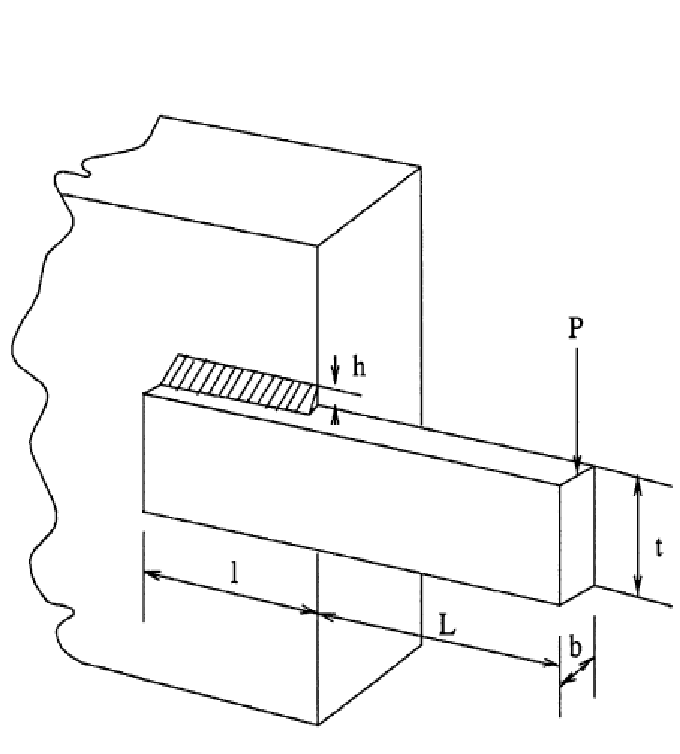
\includegraphics[width=0.55\textwidth, height=0.4\textwidth]
{welded_beam}   
\caption{Welded beam design} 
\label{fig:welded_beam_image}
\end{figure}


\newpage
%-----------------------------------------------------------

The beam is made of 1010 steel and must be supported by an 
upper and a lower weld when a constant load $P = 6000$ lb is 
applied at distance $L = 14 \hspace{2mm} in$ from the rigid 
body. The fabrication cost of the welds is given by the 
equation:
$$ f_{w} = (c_{1} + c_{2})h^{2}l$$
\\[-0.4cm]
where $c_{1}$ is the cost per unit volume of the weld 
material, $c_{2}$ the labour cost per unit weld volume and 
$V_{w} = h^{2}l$ the volume of the weld material.

The fabrication cost of the beam is proportional to the 
amount of material in the beam:
$$ f_{b} = c_{3}tb(L + l) = c_{3}tb(14.0 + l)$$
\\[-0.3cm]
where $c_{3}$ is the cost per unit volume of the beam and 
$V_{b} = tb(L + l)$ the respective volume. The construction 
costs $c_{1}, c_{2}, c_{3}$ have been estimated:
\begin{itemize}
\item For the welds: \\ 
\( c_{1} = 0.10471 \hspace{2mm} \dfrac{\$}{in^{3}} \) and 
\( c_{2} = 1 \hspace{2mm} \dfrac{\$}{in^{3}} \)
\item For the beam: \\ 
\( c_{3} = 0.04811 \hspace{2mm} \dfrac{\$}{in^{3}} \)
\end{itemize} 
\vspace{2mm}
The overall fabrication cost can be written as:
\begin{equation}
f_{tot} = f_{w} + f_{b} = 1.10471h^{2}l + 0.04811tb(14.0 + l)
\end{equation}

The stress states that describe the optimization case are 
subsequently defined and will serve as the imposed 
constraints. The first is the shear stress of the welds that must 
not exceed the maximum allowable shear stress of the material 
$τ_{max} \leq 13600$ psi. The shear stress of the welds is defined 
as such:
\begin{equation}\label{welded_con1}
τ = \sqrt{ τ_{p}^{2} + 2τ_{p}τ_{t}cosθ + τ_{t}^{2} } 
\xrightarrow{cosθ = l/2R} 
\sqrt{ τ_{p}^{2} + \dfrac{lτ_{p}τ_{t} }{R} + τ_{t}^{2} } 
\end{equation}
\\[-0.2cm]
where $R$ is the distance from the center of the 
cross-section of the beam, $τ_{p}$ the primary stress of the 
weld throat and $τ_{t}$ the torsional stress developed on the 
beam due to the torque $M$ developed by the applied load $P$ 
at its end. The equations describing the aforementioned 
static mechanical phenomena are the following:
\begin{equation}
\begin{split}
& R = \sqrt{\dfrac{l^{\hspace{0.5mm}2}}{4} + \left( 
\dfrac{h + t}{2} \right)^{2} } 
\\[0.2cm] &
τ_{p} = \dfrac{P}{\sqrt{2}hl} = \dfrac{6000}{\sqrt{2}hl}
\\[0.3cm] &
τ_{t} = \dfrac{MR}{J}
\\ & 
M = P\left(L + \dfrac{l}{2} \right) = 6000 \left(14.0 + 
\dfrac{l}{2} \right)
\end{split}
\end{equation}

\newpage
%-------------------------------------------------------

In torsional stress equation, the variable $J$ is the polar 
moment of inertia of the weld:
$$ J = 2\sqrt{2}hl \left[ \dfrac{l^{\hspace{0.5mm}2}}{12} + 
\left( \dfrac{h + t}{2} \right)^{2}  \right]$$ 
\\
The second stress that affects the quality of the design is 
the normal bending stress of the beam that must not exceed 
the maximum yield strength of the material $σ_{max} \leq 
30000$ psi and is equal to:

\begin{equation}\label{welded_con2}
σ = \dfrac{6PL}{bt^{2}} = \dfrac{504000}{bt^{2}}
\end{equation} 
\\[-0.1cm]
The deflection at the end of the beam is the next constraint 
that must be incorporated into the optimization of the welded 
beam. The deflection of a cantilever beam of length 
$L = 14 \hspace{2mm} in$ must not exceed $δ_{max} \leq 
0.25 \hspace{2mm} in$ and is calculated as such:

\begin{equation}\label{welded_con4}
δ = \dfrac{4PL^{3}}{Ebt^{3}} = \dfrac{2.1952}{bt^{3}}
\end{equation} 
\\[-0.2cm]
where $E$ is the Young's modulus; for 1010 steel is equal
to $30 \times 10^{6}$ psi.

Additionally, the structural integrity of the beam requires 
that the buckling load in the vertical direction must be
greater than the applied load $P = 6000$ psi. The critical 
buckling load of the beam is calculated as such:

\begin{equation}\label{welded_con5}
P_{c} = \dfrac{4.013 \sqrt{\dfrac{EGt^{2}b^{6}}{36}}}{L^{2}}
\left( 1 - \dfrac{t}{2L} \sqrt{\dfrac{E}{4G}} \right)
\end{equation}
\\
where $G$ is shearing modulus; for steel 1010 is equal to 
$G = 12 \times 10^{6}$ psi. 

It is evident that the thickness of the welds $h$ should not
exceed the width of the beam and therefore the last imposed
constraint is $h \leq b$. Consequently, the optimization of 
the welded beam design requires the minimization of a single 
objective, i.e. the fabrication cost of the structural design,
in the 4-dimensional space formed by the design 
variables $\vec{β} = \left( β_{1}, β_{2}, β_{3}, β_{4} \right)\!
= \!\left( h, l, t, b \right) \in \mathbb{R}^{4}$ and bounded 
by the 5 imposed constraints. 

\begin{equation}
\begin{split}
min \hspace{2mm} & f(\vec{β}) = 1.10471β_{1}^{2}β_{2} + 
0.04811β_{3}β_{4}(14.0 + β_{2}) 
\\[0.2cm] 
\text{subject to} \hspace{2mm} & c_{1}(\vec{β}) = 
τ(\vec{β}) - τ_{max} \leq 0 
\\ &
c_{2}(\vec{β}) = σ(\vec{β}) - σ_{max} \leq 0
\\ &
c_{3}(\vec{β}) = β_{1} - β_{4} \leq 0
\\ &
c_{4}(\vec{β}) = δ(\vec{β}) - δ_{max} \leq 0
\\ &
c_{5}(\vec{β}) = P - P_{c}(\vec{β}) \leq 0
\end{split}
\end{equation}
\\
where the bounds of each design variable are $0.125 \leq 
β_{1} \leq 10.0$, $0.1 \leq β_{2} \leq 10.0$, $0.1 \leq β_{3} 
\leq 10.0$ and $0.1 \leq β_{4} \leq 10.0$. The formulas that 
describe $τ(\vec{β})$, $σ(\vec{β})$, $δ(\vec{β})$ and 
$P_{c}(\vec{β})$ can be found in equations \ref{welded_con1}, 
\ref{welded_con2}, \ref{welded_con4} and \ref{welded_con5}, 
respectively.

\newpage

%-----------------------------------------------------------
%-------EAs----------
%------------------------------------------------------
\begin{itemize}
\item \textbf{Optimization using EAs}
\end{itemize}

First, the welded beam design is optimized using plain EAs 
that utilise the problem-specific evaluation model. The 
optimization is performed using EASY software in order to 
identify the most suitable values for the parameters of the 
evolution, e.g. offspring and parents population size, mutation 
probability and crossover scheme. The evolution parameters 
identified via the use of EAs are later used to facilitate the 
evolution in MAEA-based optimization. The number of offspring and 
parent population is set to $(μ,λ) = (20, 60)$ where 4 parents are 
combined to create a single offspring with one-point crossover. 
Gray binary encoding is used and 15 bits are assigned to each 
design variable. The optimization phase terminates after 27000 
PSM evaluations have been performed and is repeated for 5 
randomly initialised offspring populations $P_{λ}^{0}$ via the use 
of a Random Number Generator (RNG). The results are presented in 
table \ref{table:EAs_welded_beam} and in figure 
\ref{fig:EAs_welded_beam}.

\begin{table}[h!]
\centering
%\rowcolors{2}{gray!30!}{white!50!gray!10}
\scalebox{0.85}{%
\begin{tabular}[c]{ |p{1cm}||p{1.5cm}|p{1.2cm}|p{1.2cm}|
p{1.8cm}|p{1.6cm}|}
\toprule
\multicolumn{6}{|c|}{\cellcolor{gray!30!} 
\textbf{Welded beam case}} \\
\midrule 
& $(μ,λ)$ \textbf{population} & \textbf{Best} & 
\textbf{Worst} & \textbf{Average} & \textbf{Average PSM eval.} \\
\hline
\textbf{EAs} & (20, 60) & 2.38 & 2.49 & 2.43 & 27000 \\
\bottomrule
\end{tabular}%
}
\caption{Optimization of welded beam design using EAs}
\label{table:EAs_welded_beam}
\end{table}

\begin{figure}[h!]
\centering
	\begin{subfigure}[b]{0.49\textwidth}
    \centering
    \caption{Comparison between the convergence histories of 5 
    different $λ$ initializations}
    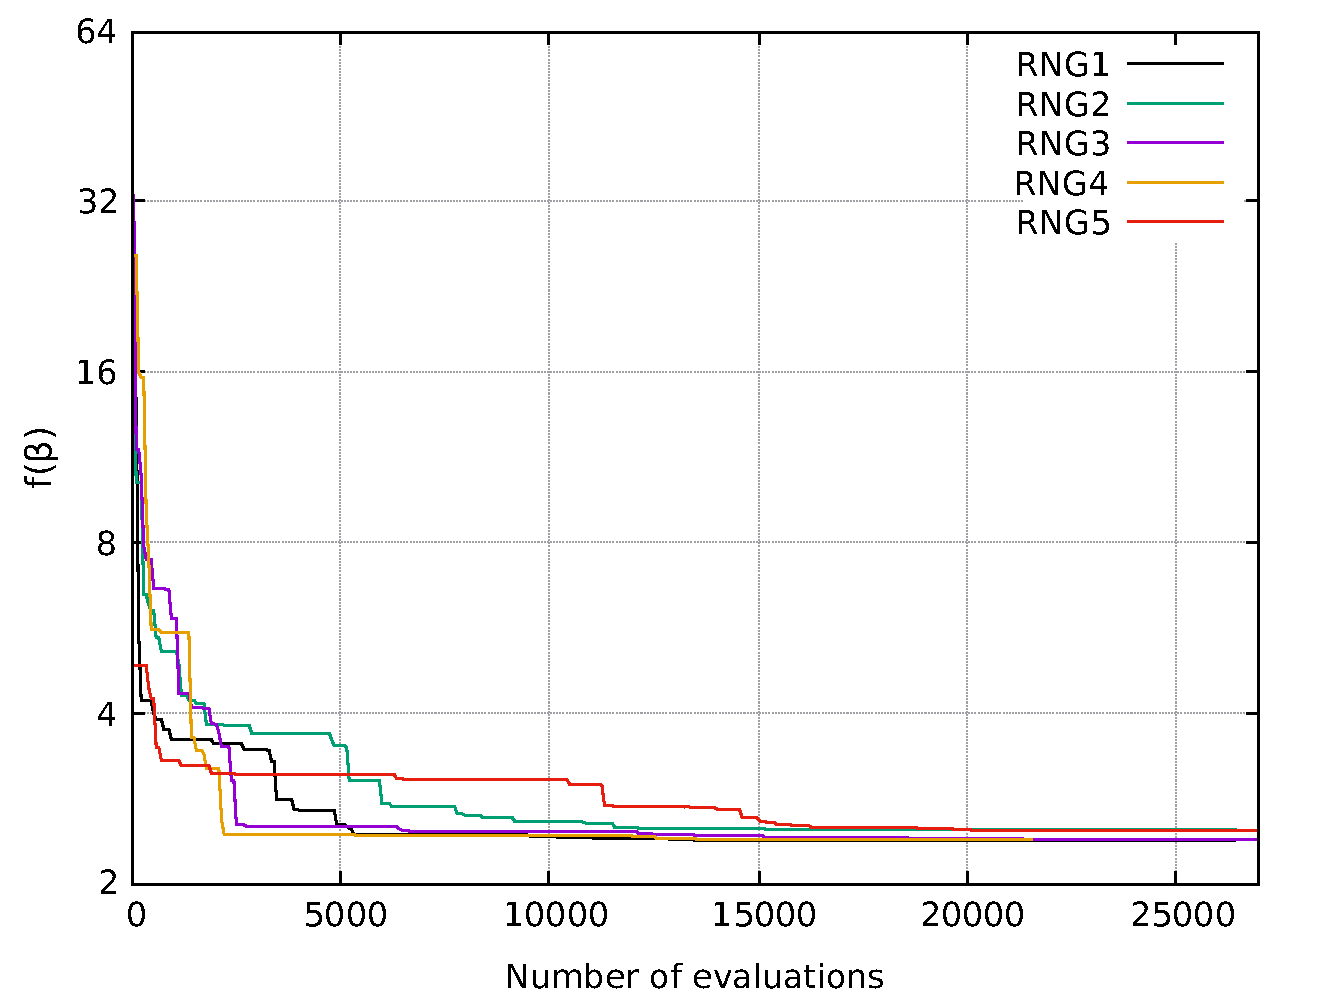
\includegraphics[width=\textwidth, height=0.28\textheight, 
    scale=1.0]{welded_beam_ea.pdf}    
    \end{subfigure}
    \hfill
    \begin{subfigure}[b]{0.49\textwidth}
    \centering
    \caption{Convergence history of the optimal run}
    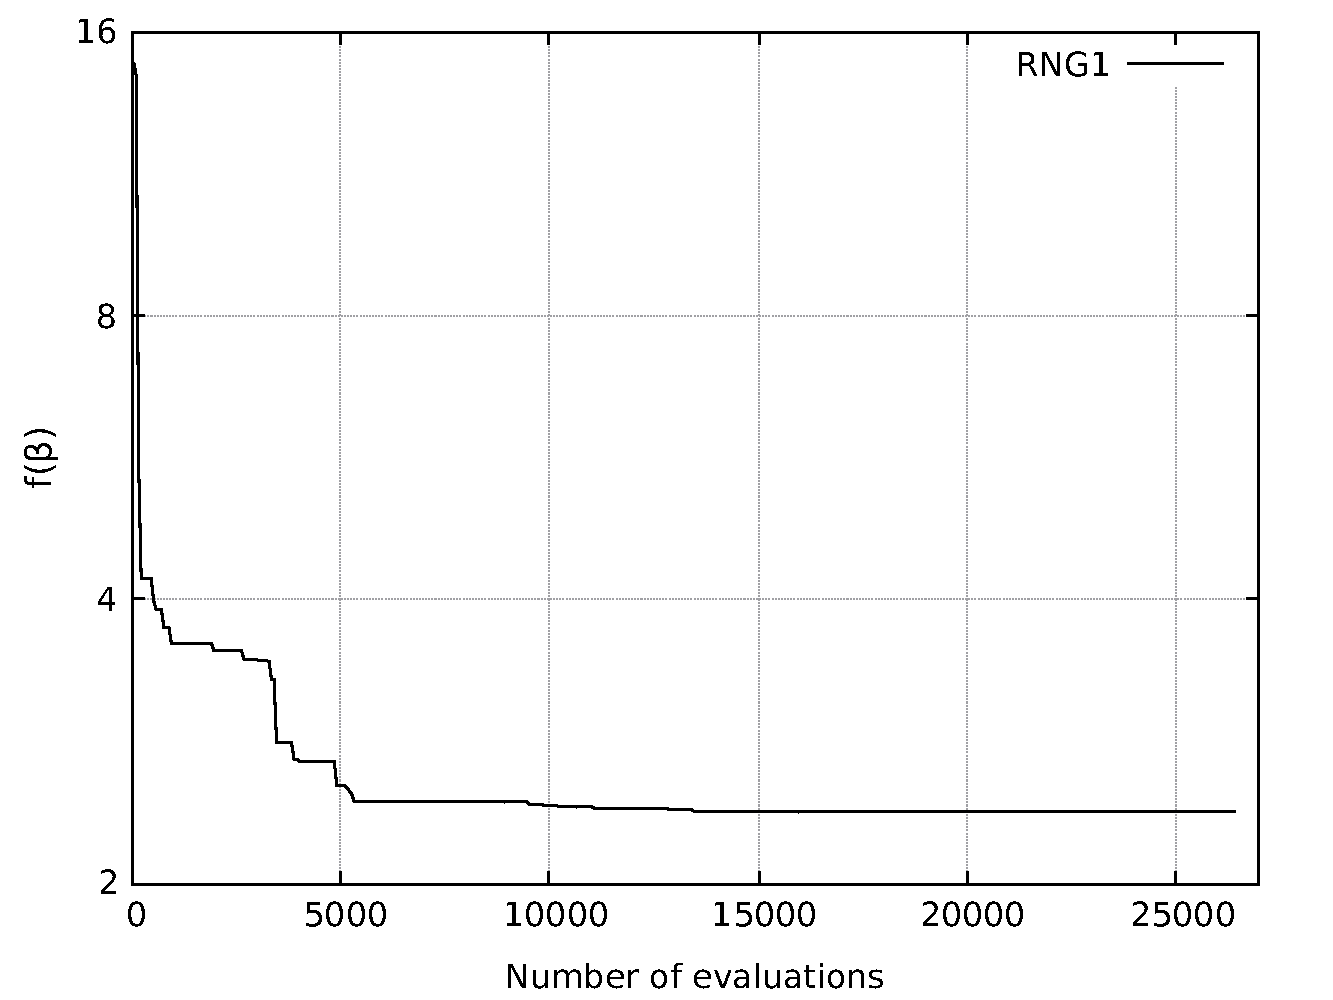
\includegraphics[width=\textwidth, height=0.28\textheight, 
    scale=1.0]{welded_beam_ea_best.pdf}    
    \end{subfigure}  
\caption{Convergence history of welded beam optimization case 
using EAs} 
\label{fig:EAs_welded_beam}
\end{figure}

The design variable vector that minimizes the construction
cost of the welded beam using plain EAs initialized via RNG1 is 
$\vec{β} = [0.244, 6.194,$ $8.329, 0.244]$. 

\newpage

%---------------------------------------------------------
%---------Off line------------
%----------------------------------------------------------

\begin{itemize}
\item \textbf{Optimization using MAEAs with off-line trained 
metamodels}
\end{itemize}

In MAEAs using off-line trained metamodels, both the 
objective $\mathbf{F}(\vec{β})$ and the imposed constraints 
$\mathbf{C}(\vec{β}) = [\vec{c}_{1}, \vec{c}_{2}, \hdots, 
\vec{c}_{n_{t}}]^{T}$, where $\vec{c}_{i} = [c_{i,1},
 c_{i,2}, \hdots, c_{i,n_{c}}]$, are approximated using 
surrogate models. Specifically, a global metamodel is built 
on the single objective and $n_{c}$ unique metamodels on each 
imposed constraint. In this case, the objective function is 
approximated by a KPLS model, while each constraint is 
approximated via the use of Kriging model; responsible for the 
construction of the aforementioned metamodels is SMT software. 
Alternatively, a single surrogate model can be trained to 
approximate the entirety of the constraints but this approach 
resulted in a poorly trained surrogate model. However, even the 
first approach resulted in surrogate models with poor overall 
fitting, especially when approximating a function with design 
variables in the denominator that tend to zero. To solve this 
issue an approach is proposed where constraints with denominators 
that tend to 0 are reduced to polynomials. Let the original 
approach of unmodified constraints be case 1 and let the modified 
approach be case 2, then:

\begin{equation}
\begin{split}
& c_{1}(\vec{β}) =  \sqrt{ τ_{p}^{2} + 
\dfrac{τ_{p}τ_{t}β_{2}}{R} + τ_{t}^{2} } - τ_{max} \leq 0
\Rightarrow \hspace{2mm}
τ_{p}^{2} + \dfrac{τ_{p}τ_{t}β_{2}}{R} + τ_{t}^{2} \leq 
τ_{max}^{2} \xrightarrow{R > 0}
\\[0.3cm] &
τ_{p}τ_{t}β_{2} \leq - R \left[ τ_{p}^{2} + τ_{t}^{2} - τ_{max}
^{2} \right] \xrightarrow{τ_{p}τ_{t}β_{2} > 0}\hspace{1mm}
c_{1}(\vec{β})_{new} = \dfrac{R \left[τ_{p}^{2} + τ_{t}^{2} -
τ_{max}^{2} \right] }{τ_{p}τ_{t}β_{2}}  - 1 \leq 0
\end{split}
\end{equation}
\\[-0.4cm]
\begin{equation}\label{con2_mod}
c_{2}(\vec{β}) = \dfrac{6PL}{β_{4}β_{3}^{2}} -σ_{max} \leq 0 
\xrightarrow{β_{3}, β_{4} > 0} c_{2}(\vec{β})_{new} = 
6PL - σ_{max}β_{4}β_{3}^{2} \leq 0
\end{equation}
\\[-0.2cm]
\begin{equation}\label{con4_mod}
c_{4}(\vec{β}) = \dfrac{4PL^{3}}{Eβ_{4}β_{3}^{3}} - δ_{max} 
\leq 0 \xrightarrow{β_{3}, β_{4} > 0} c_{4}(\vec{β})_{new} = 
4PL^{3} - δ_{max}Eβ_{4}β_{3}^{3} \leq 0
\end{equation}
\vspace{-2mm}

\begin{figure}[h!]
\centering
\begin{subfigure}[b]{0.49\textwidth}
    \centering
    \caption{Case 1: Comparison between $c_{4}(\vec{β})$ and 
    $\widehat{c}_{4}(\vec{β})$} 
    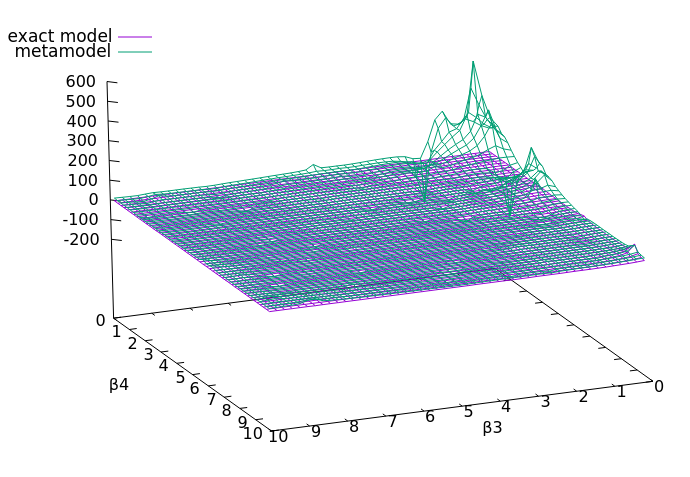
\includegraphics[width=\textwidth, height=0.75\textwidth, 
    scale=1]{con4_welded_beam_before.png}    
    \end{subfigure}
    \hfill
    \begin{subfigure}[b]{0.49\textwidth}
    \centering 
    \caption{Case 2: Comparison between $c_{4}(\vec{β})$ and 
    $\widehat{c}_{4}(\vec{β})$}
    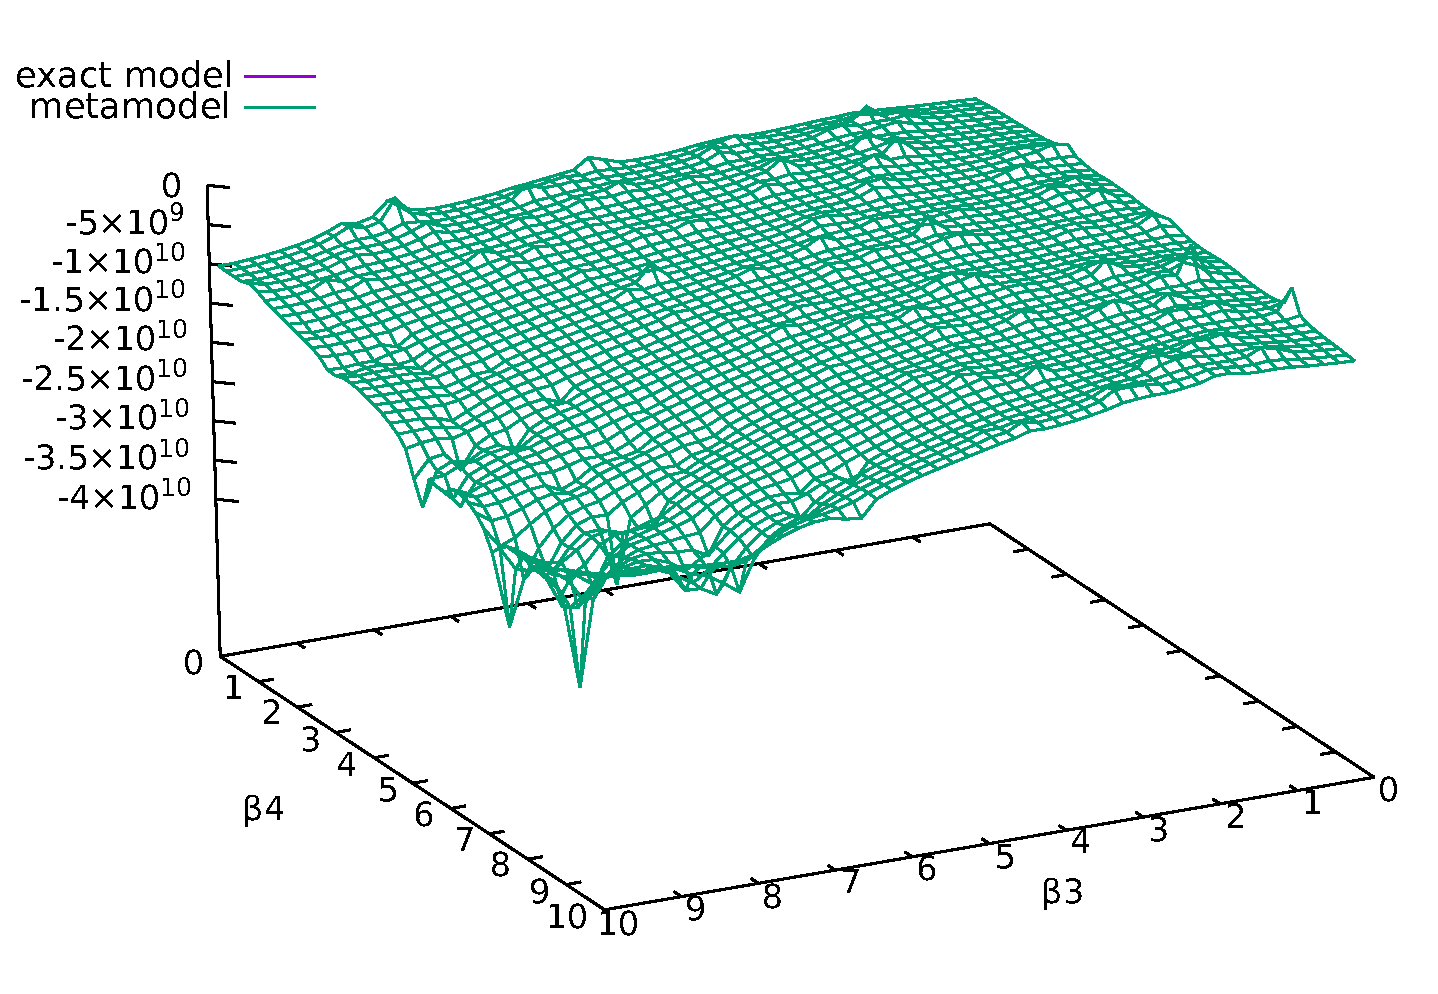
\includegraphics[width=\textwidth, height=0.75\textwidth, 
     scale=1]{con4_welded_beam_after.pdf} 
    \end{subfigure}
\caption{Error of the metamodel when approximating the original 
NRMSE = 1.206111 (left) and the modified NRMSE = $1.182408 \!
\cdot \! 10^{-6}$ (right) equation $c_{4}(\vec{β})$ using an 
LHD composed of $n_{t} = 240$ training patterns}
\label{fig:mod_c4} 
\end{figure}

\newpage
%----------------------------------------------------------


\begin{figure}[h!]
\centering
	\begin{subfigure}[b]{0.49\textwidth}
    \centering
    \caption{Case 1: $c_{2}(\vec{β})$ function}
    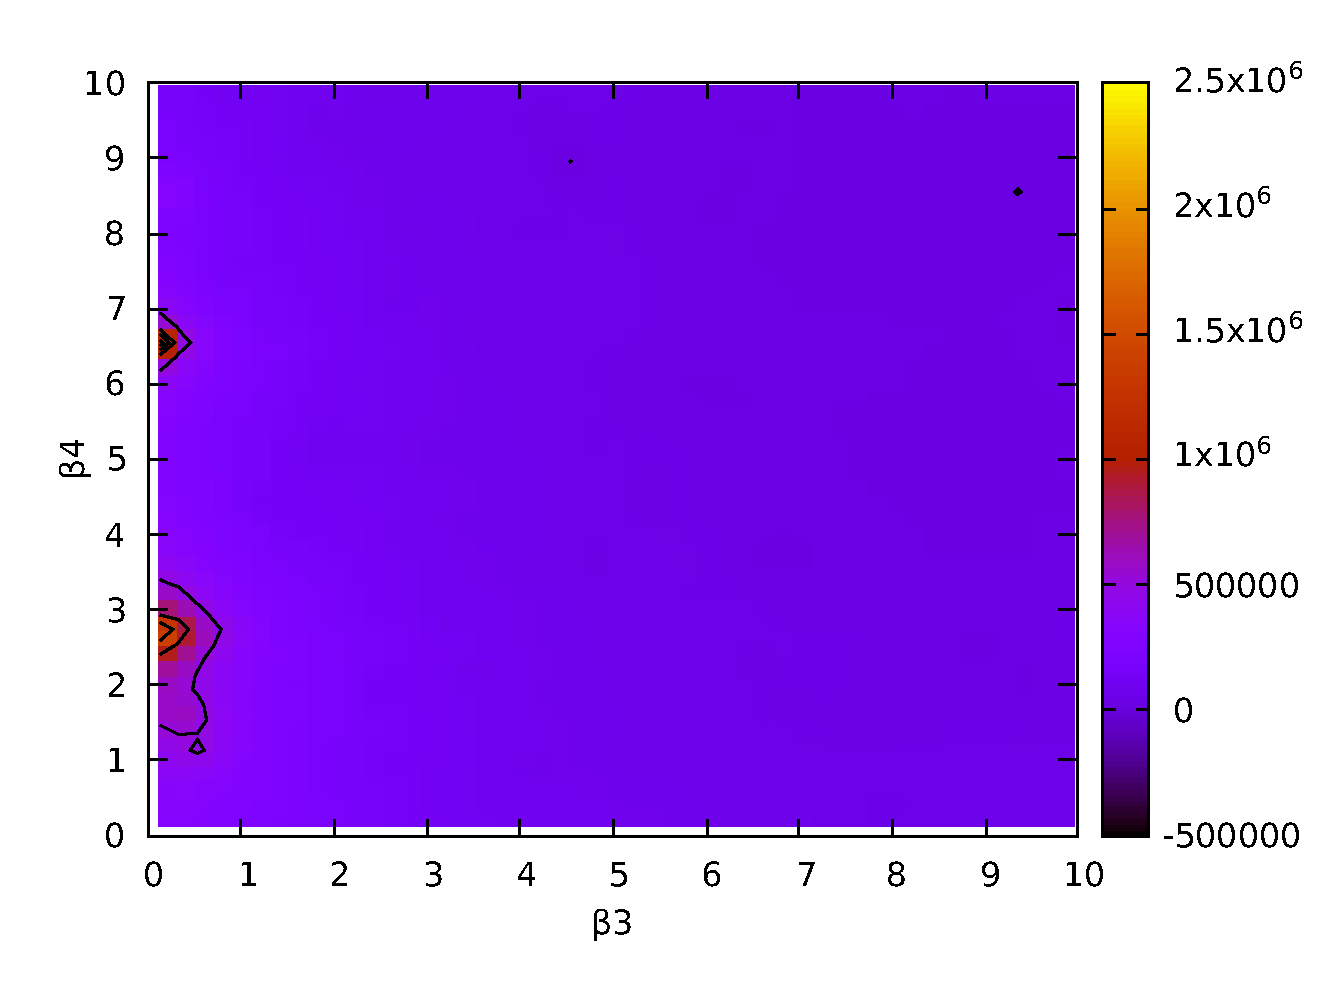
\includegraphics[width=\textwidth, height=0.9\textwidth, 
    scale=1]{con2_welded_beam_contour_before.pdf}    
    \end{subfigure}
    \hfill
    \begin{subfigure}[b]{0.49\textwidth}
    \centering 
    \caption{Case 2: $c_{2}(\vec{β})$ function}
    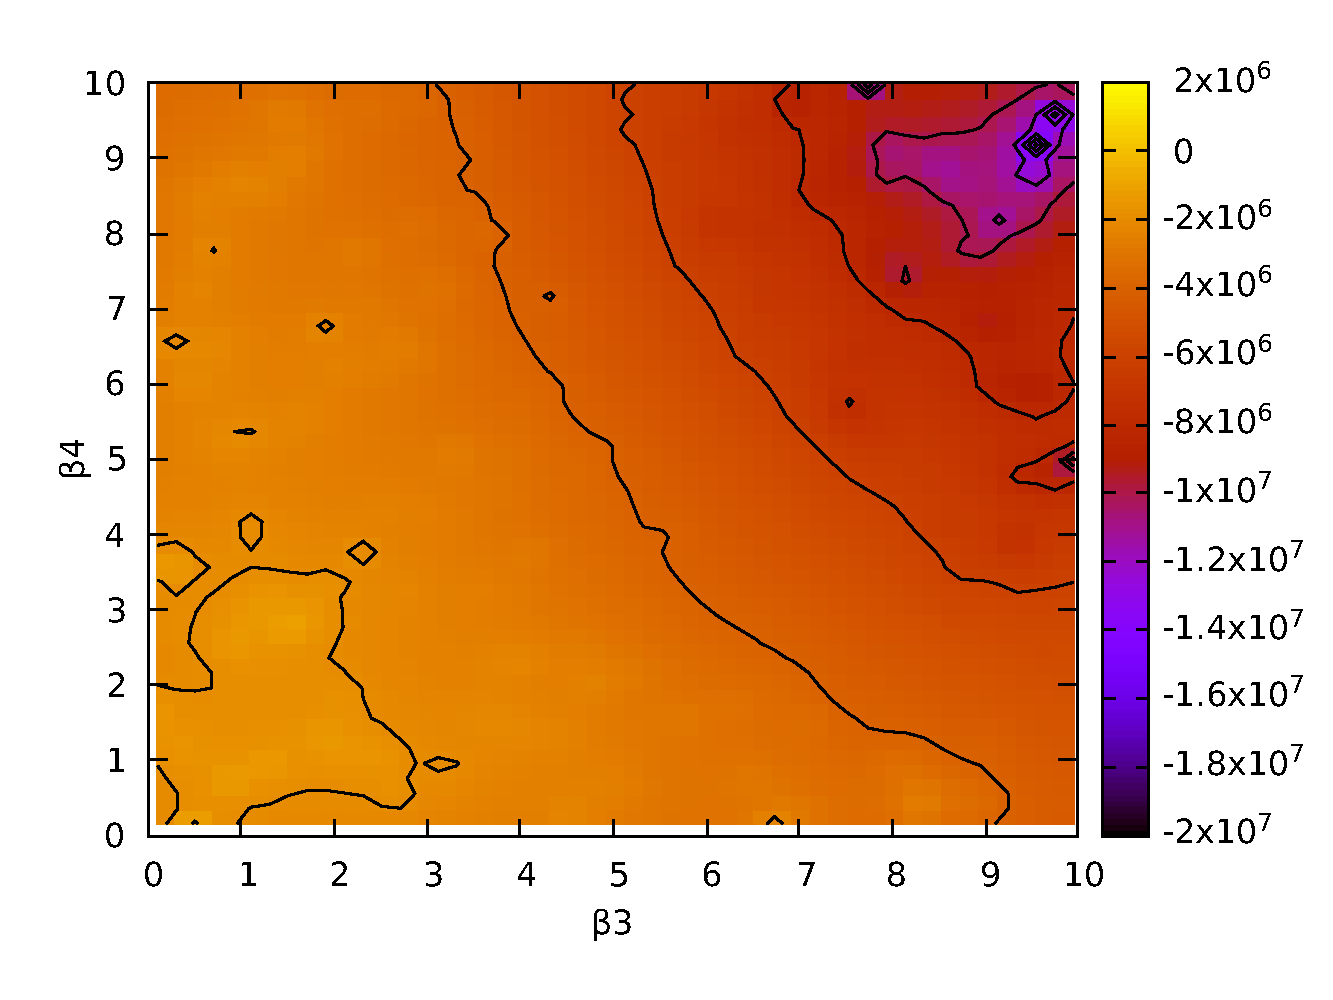
\includegraphics[width=\textwidth, height=0.9\textwidth, 
     scale=1]{con2_welded_beam_contour_after1.pdf} 
    \end{subfigure}
    \hfill
    \begin{subfigure}[b]{0.49\textwidth}
    \centering
    \caption{Case 1: Prediction $\widehat{c}_{2}(\vec{β})$ 
    function}
    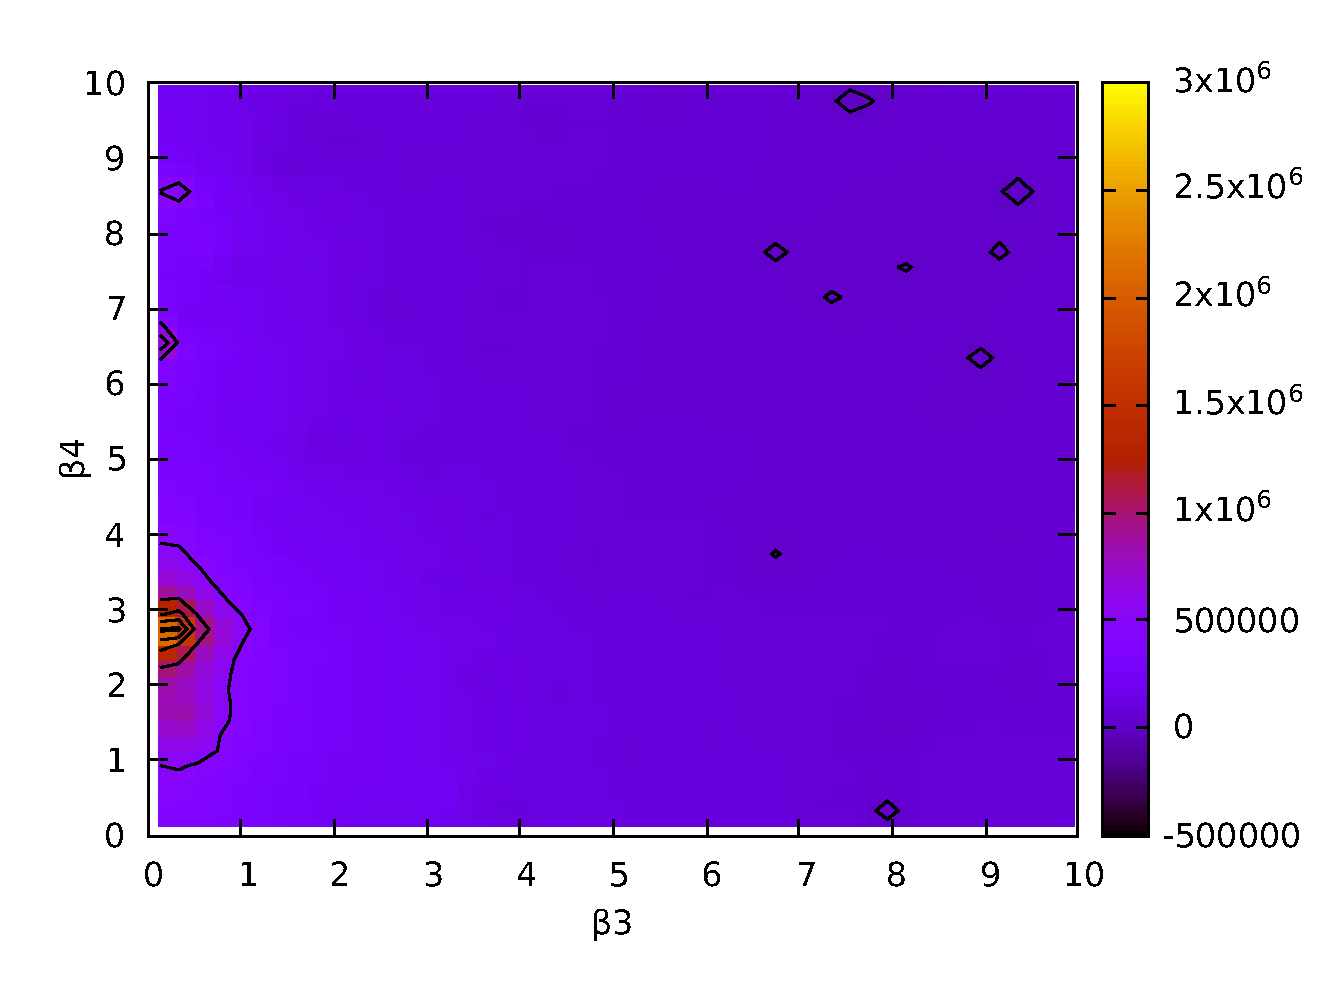
\includegraphics[width=\textwidth, height=0.9\textwidth, 
    scale=1]{con2_welded_beam_contour_before_metamodel.pdf}    
    \end{subfigure}
    \hfill
    \begin{subfigure}[b]{0.49\textwidth}
    \centering 
    \caption{Case 2: Prediction $\widehat{c}_{2}(\vec{β})$}
    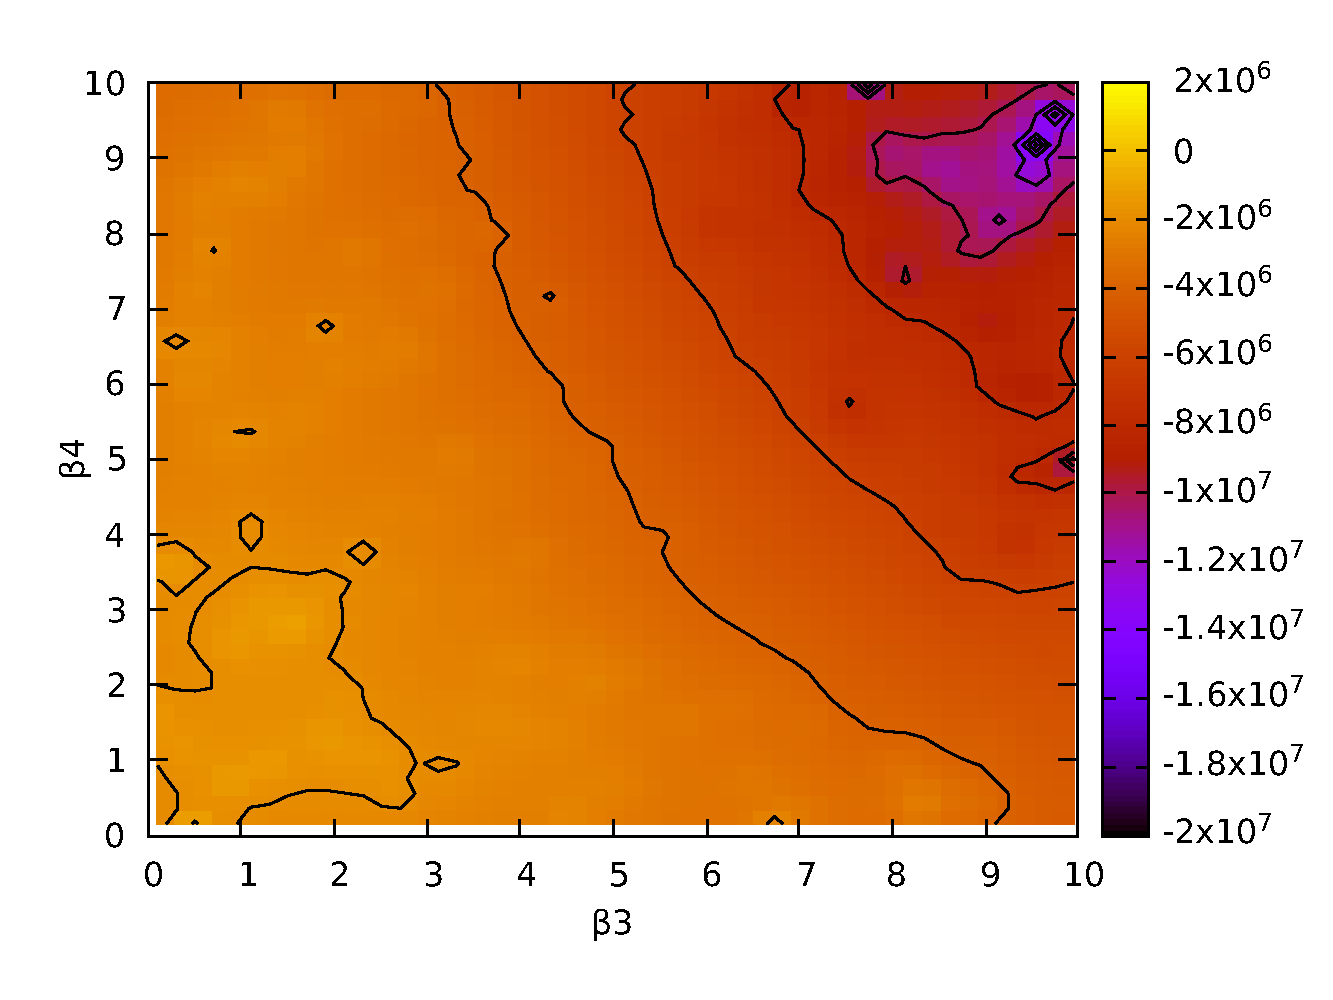
\includegraphics[width=\textwidth, height=0.9\textwidth, 
     scale=1]{con2_welded_beam_contour_after1.pdf} 
    \end{subfigure}
\caption{Contour projections to 2D plane for the original 
(left) and modified (right) function of the 2nd constraint}
\label{fig:mod_c2} 
\end{figure}

In both figures, i.e. \ref{fig:mod_c4} and \ref{fig:mod_c2},
the visualization of the constraint function justifies the 
initial assumption of underfitted metamodels built $\forall 
\vec{β} \in \mathbb{R}^n_{β}$ when $β_{1}, β_{4} \rightarrow 0$; 
such metamodels are trained in case 1. In case 2, the modification 
in constraints $c(\vec{β}_{1}), c(\vec{β}_{2})$ and $c(\vec{β}
_{4})$ results in a better model fitting, NRMSE = $1.182408 \!
\cdot \! 10^{-6}$ compared to NRMSE = 1.206111 of case 1. 
The minimization of the welded beam case that through 5 runs is 
presented in table \ref{table:offline_case2_welded_beam}, where a 
maximum of 5000 evaluations per cycle are performed using MAEAs 
with off-line trained metamodels:

\begin{table}[h!]
\centering
%\rowcolors{2}{gray!30!}{white!50!gray!10}
\scalebox{0.84}{%
\begin{tabular}[c]{ |p{3.4cm}||p{1.5cm}|p{1.2cm}|p{1.2cm}|
p{1.8cm}|p{2.3cm}|p{1.3cm}|}
\toprule
\multicolumn{7}{|c|}{\cellcolor{gray!30!} 
\textbf{Case 2}} \\
\midrule 
& $(μ,λ)$ \textbf{population} & \textbf{Best} & 
\textbf{Worst} & \textbf{Average} & \textbf{Avg. metamodel 
eval./cycle} & 
\textbf{Avg. cycles} \\
\hline
\textbf{MAEAs, off-line} & (20, 60) & 2.35 & 2.56 & 2.44 
& 3168 & 3 \\
\bottomrule
\end{tabular}%
}
\caption{Optimization of welded beam design using MAEAs with 
off-line training}
\label{table:offline_case2_welded_beam}
\end{table}

\newpage
%------------------------------------------------------------


The optimal candidate solution obtained via this method is 
$\vec{β} = [0.336, 5.067,$ $7.323, 0.338]$. The corresponding 
value of each constraint and objective is presented in table 
\ref{table:offline_case2_deviation_welded_beam}.

\begin{table}[h!]
\centering
%\rowcolors{2}{gray!30!}{white!50!gray!10}
\scalebox{0.83}{%
\begin{tabular}[c]{ |p{1.6cm}||p{2cm}p{1.8cm}p{1.4cm}
p{2.4cm}p{1.6cm}p{1cm}|}
\toprule
\rowcolor{gray!30!}
\textbf{Case 2} & $\mathbf{c_{1}}(\vec{\bm{β}})$ 
& $\mathbf{c_{2}}(\vec{\bm{β}})$ 
& $\mathbf{c_{3}}(\vec{\bm{β}})$ 
& $\mathbf{c_{4}}(\vec{\bm{β}})$ 
& $\mathbf{c_{5}}(\vec{\bm{β}})$ 
& $\mathbf{f}(\vec{\bm{β}})$ \\
\midrule
\textbf{MAEAs} & -0.412243 & -29020.84 & -0.019 
& -1065388211 & -276.80 & 2.35 \\
\textbf{PSM} & 1129.41 & -1633.52 & -0.019 
& -0.235446 & -261.95 & 2.35 \\
\bottomrule
\end{tabular}%
}
\caption{\textbf{C}, \textbf{F} responses to $\vec{β}$ found 
via MAEAs with off-line training in case 2}
\label{table:offline_case2_deviation_welded_beam}
\end{table}

MAEAs with off-line training utilizing the approach of modified 
constraints (case 2) converge in candidate solutions that 
violate the first constraint $c_{1}(\vec{β})$. In order to 
determine the extent to which the design space has changed, the 
aforementioned approach is implemented in plain EAs that 
utilize the modified problem-specific model, denoted by 
$\mathrm{PSM}^{'}$ for simplicity. If $\mathrm{PSM}^{'}$-based 
EAs converge to an optimal solution that lies in the design 
space of the original PSM, then the modification in 
constraints did not lead to a significant change in the design 
space of candidate solutions and the unsatisfactory solutions 
are contributed to metamodel-related flaws. EAs using 
$\mathrm{PSM}^{'}$ find the optimal solution $\vec{β} = 
[0.272, 4.300, 7.856, 0.272]$. The corresponding value of each 
constraint and objective is presented in table 
\ref{table:offline_case2_PSM_welded_beam}

\begin{table}[h!]
\centering
%\rowcolors{2}{gray!30!}{white!50!gray!10}
\scalebox{0.83}{%
\begin{tabular}[c]{ |p{1.4cm}||p{2cm}p{1.8cm}p{1.2cm}
p{2.2cm}p{1.8cm}p{1cm}|}
\toprule
\rowcolor{gray!30!}
\textbf{Case 2} & $\mathbf{c_{1}}(\vec{\bm{β}})$ 
& $\mathbf{c_{2}}(\vec{\bm{β}})$ 
& $\mathbf{c_{3}}(\vec{\bm{β}})$ 
& $\mathbf{c_{4}}(\vec{\bm{β}})$ 
& $\mathbf{c_{5}}(\vec{\bm{β}})$ 
& $\mathbf{f}(\vec{\bm{β}})$ \\
\midrule
$\mathbf{PSM^{'}}$ & -0.000037 & -273.75 & 0 
& -963206327 & -529.75 & 2.15 \\
\textbf{PSM} & 3445.91 & -16.286 & 0 
& -0.234001 & -529.75 & 2.15 \\
\bottomrule
\end{tabular}%
}
\caption{\textbf{C}, \textbf{F} responses to $\vec{β}$ found 
via EAs using the $\mathrm{PSM}^{'}$}
\label{table:offline_case2_PSM_welded_beam}
\end{table}

The implemented modifications seem to distort the design space
significantly, since the optimal solution results in a design 
with welds that undergo massive shear stress $c_{1}(\vec{β}) = 
17045.91$ psi. Consequently, optimal solutions found in 
case 2 do not satisfy the constraints imposed on the design 
space and result in a unsatisfactory welded beam design. 
However, metamodels trained off-line on the PSM do not 
converge to an optimal solution due to poor constraint model 
fitting. For this reason, a new approach is proposed, 
referred to as case 3, and is based on the observation that 
the entirety of optimal solutions found via the use both the 
$\mathrm{PSM}^{'}$ and metamodels trained on the $\mathrm{PSM}
^{'}$(case 2) do not satisfy the first constraint $c_{1}
(\vec{β})$. In case 3, therefore, constraints $c_{2}, c_{4}$ 
are modified according to equations \ref{con2_mod} and 
\ref{con4_mod}, respectively, and the corresponding problem-
specific model is denoted by $\mathrm{PSM}^{''}$. The 
implementation of EAs via the use of $\mathrm{PSM}^{''}$ 
yields the optimal solution $\vec{β} \!= \![0.279, 5.679, 7.698, 
0.284]$. The corresponding value of each constraint and objective 
is presented in table \ref{table:offline_case3_PSM_welded_beam}.

\begin{table}[h!]
\centering
%\rowcolors{2}{gray!30!}{white!50!gray!10}
\scalebox{0.83}{%
\begin{tabular}[c]{ |p{1.4cm}||p{1.6cm}p{1.6cm}p{1.4cm}
p{2.2cm}p{1.6cm}p{1cm}|}
\toprule
\rowcolor{gray!30!}
\textbf{Case 3} & $\mathbf{c_{1}}(\vec{\bm{β}})$ 
& $\mathbf{c_{2}}(\vec{\bm{β}})$ 
& $\mathbf{c_{3}}(\vec{\bm{β}})$ 
& $\mathbf{c_{4}}(\vec{\bm{β}})$ 
& $\mathbf{c_{5}}(\vec{\bm{β}})$ 
& $\mathbf{f}(\vec{\bm{β}})$ \\
\midrule
$\mathbf{PSM^{''}}$ & -13.645 & -355.91 & -0.004
& -904782848 & -2906.86 & 2.56 \\
\textbf{PSM} & -13.645 & -21.170 & -0.004
& -0.233038 & -2906.86 & 2.56 \\
\bottomrule
\end{tabular}%
}
\caption{\textbf{C}, \textbf{F} responses to $\vec{β}$ found 
via EAs using the $\mathrm{PSM}^{''}$}
\label{table:offline_case3_PSM_welded_beam}
\end{table}

\newpage
%-----------------------------------------------------------


Unlike previous approaches, $\mathrm{PSM}^{''}$-based EAs 
converge to an optimal solution that satisfies the entirety 
of the constraints imposed to the original model. Metamodels 
trained off-line on the $\mathrm{PSM}^{''}$ through 5 runs yield 
the outcome shown in table 
\ref{table:offline_case3_welded_beam}.

\begin{table}[h!]
\centering
%\rowcolors{2}{gray!30!}{white!50!gray!10}
\scalebox{0.85}{%
\begin{tabular}[c]{ |p{3.4cm}||p{1.5cm}|p{1.2cm}|p{1.2cm}|
p{1.8cm}|p{2.3cm}|p{1.3cm}|}
\toprule
\multicolumn{7}{|c|}{\cellcolor{gray!30!} 
\textbf{Case 3}} \\
\midrule 
& $(μ,λ)$ \textbf{population} & \textbf{Best} & 
\textbf{Worst} & \textbf{Average} 
& \textbf{Average metamodel eval./cycle} 
& \textbf{Avg. cycles} \\
\hline
\textbf{MAEAs, off-line} & (20, 60) & 2.90 & 3.55 & 3.12 
& 2883 & 8 \\
\bottomrule
\end{tabular}%
}
\caption{Optimization of welded beam design using MAEAs with 
off-line training}
\label{table:offline_case3_welded_beam}
\end{table}

The best solution $\vec{β} = [0.336, 5.067, 7.323, 0.338]$ obtained 
via MAEAs with off-line training, produces the constraint and 
objective function values shown in table 
\ref{table:offline_case3_deviation_welded_beam} when evaluated on 
the PSM.

\begin{table}[h!]
\centering
%\rowcolors{2}{gray!30!}{white!50!gray!10}
\scalebox{0.83}{%
\begin{tabular}[c]{ |p{1.6cm}||p{1.6cm}p{1.8cm}p{1.4cm}
p{2.2cm}p{1.6cm}p{1cm}|}
\toprule
\rowcolor{gray!30!}
\textbf{Case 3} & $\mathbf{c_{1}}(\vec{\bm{β}})$ 
& $\mathbf{c_{2}}(\vec{\bm{β}})$ 
& $\mathbf{c_{3}}(\vec{\bm{β}})$ 
& $\mathbf{c_{4}}(\vec{\bm{β}})$ 
& $\mathbf{c_{5}}(\vec{\bm{β}})$ 
& $\mathbf{f}(\vec{\bm{β}})$ \\
\midrule
\textbf{MAEAs} & -469.56 & -39385.13 & -0.002
& -928918812 & -8492.04 & 2.90 \\
\textbf{PSM} & -797.35 & -2194.43 & -0.002
& -0.233450 & -8522.98 & 2.90 \\
\bottomrule
\end{tabular}%
}
\caption{\textbf{C}, \textbf{F} responses to $\vec{β}$ found 
via MAEAs with off-line training in case 3}
\label{table:offline_case3_deviation_welded_beam}
\end{table}

Consequently, the MAEA-based optimization of the welded beam case 
is performed by utilizing metamodels built off-line exclusively on 
$\mathrm{PSM}^{''}$, since MAEAs with surrogate models trained 
off-line on $\mathrm{PSM}^{'}$ and PSM either converge to 
prohibited by the constraints solutions or they do not converge 
after performing 20 optimization cycles, respectively. The 
convergence histories of EAs using PSM, $\mathrm{PSM}^{'}$ and $
\mathrm{PSM}^{''}$ are subsequently presented in figure 
\ref{fig:convergence_PSMs} all EA methods are initialized with the 
same offspring population set $P_{λ}^{0}$ corresponding to best 
solution.

\begin{figure}[h!]
\centering
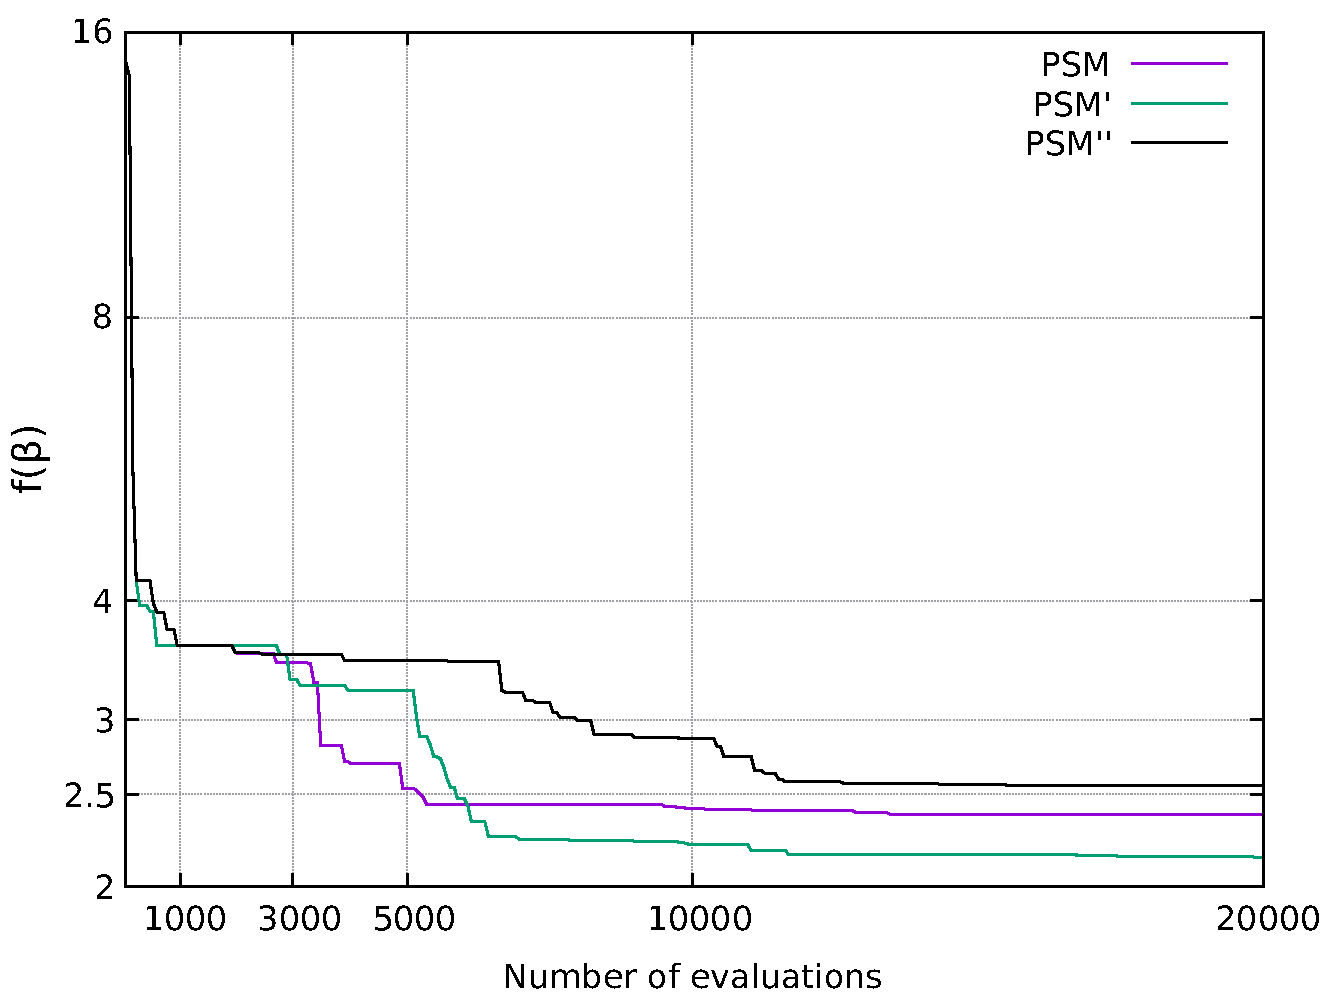
\includegraphics[width=0.6\textwidth]{EA_mod.pdf}   
\caption{Welded beam design. Comparison between the 
convergence history of EAs performing evaluations on the PSM, 
$\mathrm{PSM}^{'}$ and $\mathrm{PSM}^{''}$} 
\label{fig:convergence_PSMs}
\end{figure}

\newpage
%------------------------------------------------------------


The deviation between metamodel predicted values and evaluated 
ones, using the $\mathrm{PSM}^{''}$ of either objective function or 
some constraint, can be observed in figures 
\ref{fig:fitting_f_welded_beam}, 
\ref{fig:fitting_con1_2_welded_beam} and 
\ref{fig:fitting_con3_5_welded_beam}. The surrogate models are 
trained on $n_{t} \!= \!n_{doe} \!= \!240$ patterns $\mathbf{X}$ 
collected via the implementation of LHS that makes use of the ESE 
algorithm to construct an optimal space-filling design. At the end 
of each optimization loop, a new random design of $n_{new\_doe} \!= 
\!20$ points and 1 elite are added to the initial LHD. The 
optimization process converged after 10 cycles and, therefore, at 
the end of the optimization the metamodels are retrained on $n_{t} 
\!= \!n_{doe}^{'} \!= \!429$ patterns. Each individual $\vec{β} \!
\in \!P_{λ}^{0}$ selected in the first of the 5 total runs is used 
to validate both metamodels and calculate the NRMSE.
\vspace{-2mm}
\begin{figure}[h!]
\centering
    \begin{subfigure}[b]{0.45\textwidth}
    \centering
    \caption{Initial $f$, $\mathrm{NRMSE} \!= \!0.00000269$}
    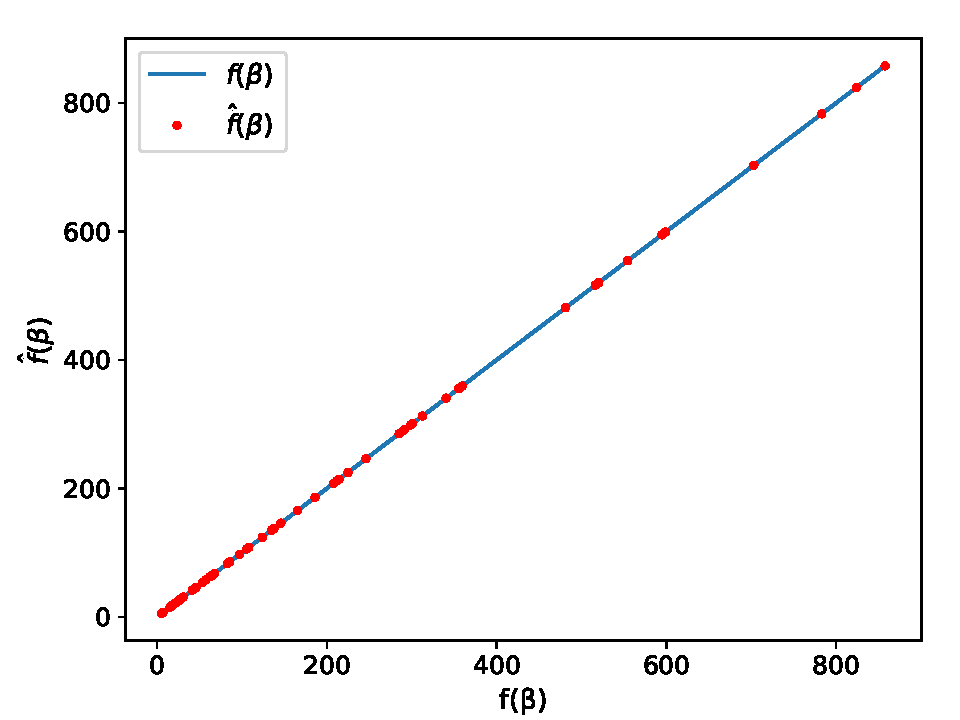
\includegraphics[width=\textwidth, height=0.6\textwidth, 
    scale=1]{welded_beam_f_fitness_start.pdf}    
    \end{subfigure}
    \hfill
    \begin{subfigure}[b]{0.45\textwidth}
    \centering
    \caption{Final $f$, $\mathrm{NRMSE} \!= \!0.00000042$}
    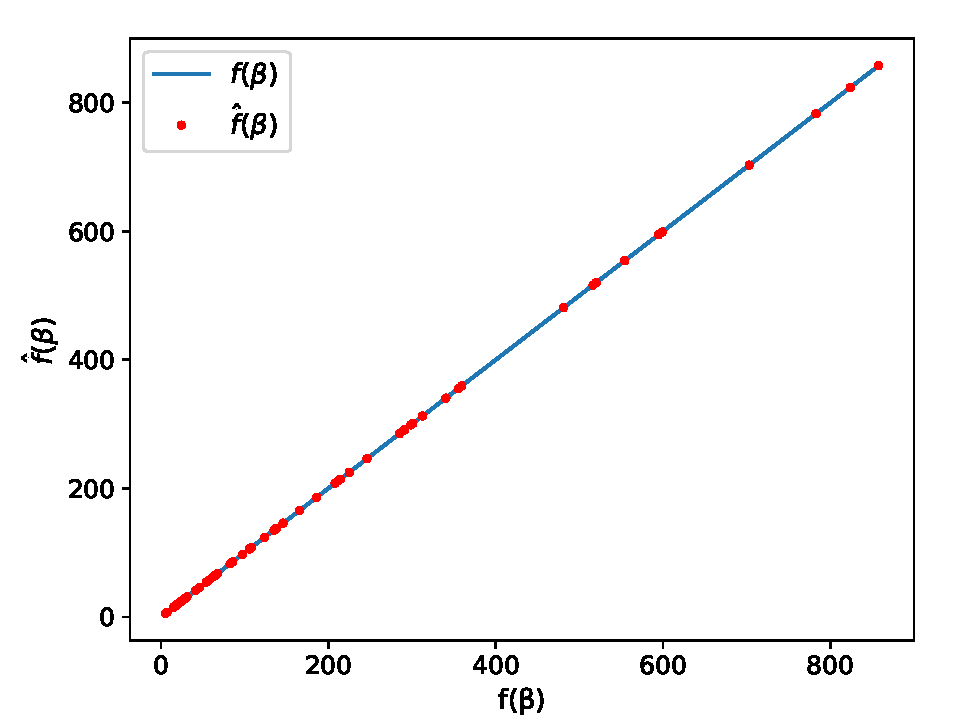
\includegraphics[width=\textwidth, height=0.6\textwidth, 
    scale=1]{welded_beam_f_fitness_end.pdf} 
    \end{subfigure}
    \caption{Case 3, welded beam case with RNG1. Deviation between 
    exact $\mathrm{PSM}^{''}$ values of the objective function 
    $\vec{f}(\vec{β})$ and KPLS predictions $\hat{\vec{f}}(\vec{β})
    $. The initial KPLS model is trained on $n_{doe} \!= \!240$ and 
    the final on $n_{doe}^{'} \!= \!429$ training patterns.}
    \label{fig:fitting_f_welded_beam}
\end{figure}
\vspace{-4mm}
\begin{figure}[h!]
\centering
    \begin{subfigure}[b]{0.45\textwidth}
    \centering
    \caption{Initial $c_{1}$, $\mathrm{NRMSE} \!= \!0.7773964$}
    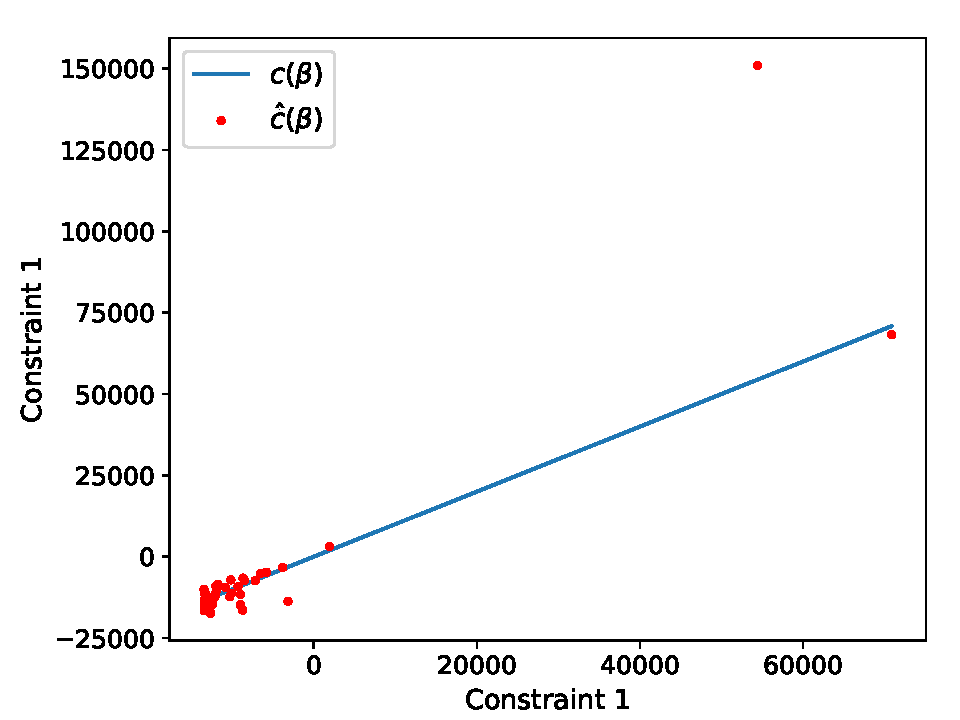
\includegraphics[width=\textwidth, height=0.58\textwidth, 
    scale=1]{welded_beam_con1_fitness_start.pdf}    
    \end{subfigure}
    \hfill
    \begin{subfigure}[b]{0.45\textwidth}
    \centering
    \caption{Final $c_{1}$, $\mathrm{NRMSE} \!= \!0.55329077$}
    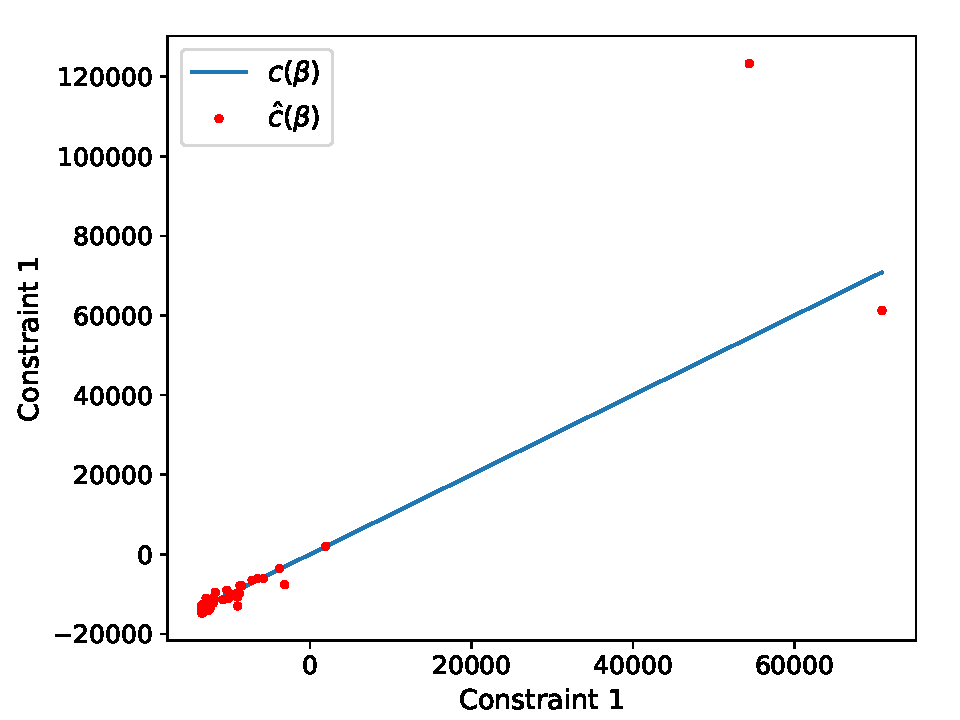
\includegraphics[width=\textwidth, height=0.58\textwidth, 
    scale=1]{welded_beam_con1_fitness_end.pdf}    
    \end{subfigure}
    \hfill
    \begin{subfigure}[b]{0.45\textwidth}
    \centering
    \caption{Initial $c_{2}$, $\mathrm{NRMSE} \!= \!0.00000249$}
    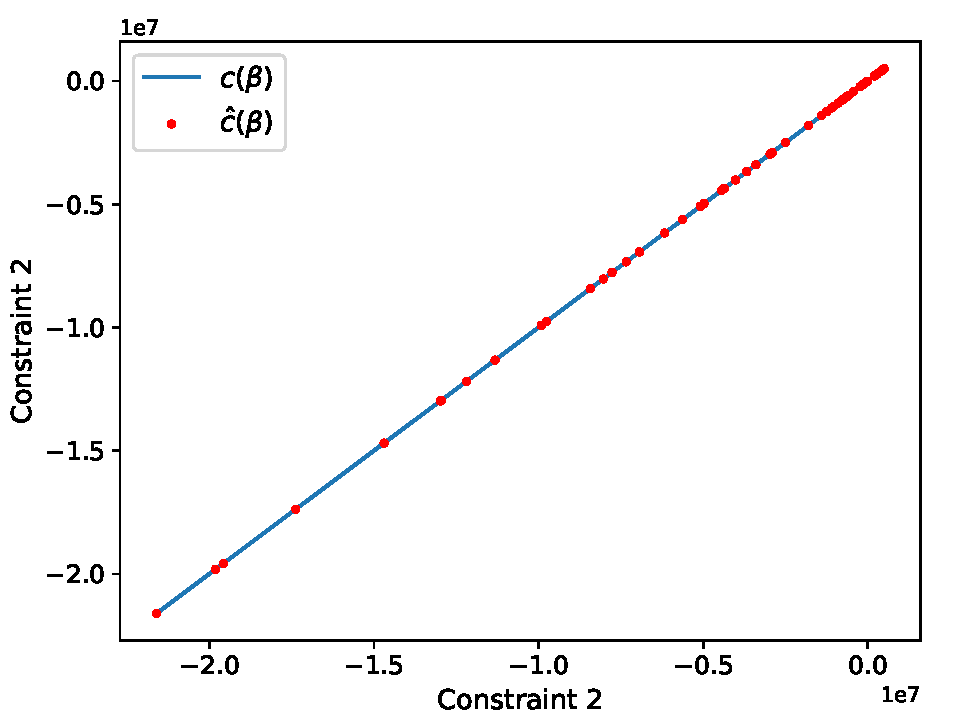
\includegraphics[width=\textwidth, height=0.58\textwidth, 
    scale=1]{welded_beam_con2_fitness_start.pdf}    
    \end{subfigure}
    \hfill
    \begin{subfigure}[b]{0.45\textwidth}
    \centering
    \caption{Final $c_{2}$, $\mathrm{NRMSE} \!= \!0.00000063$}
    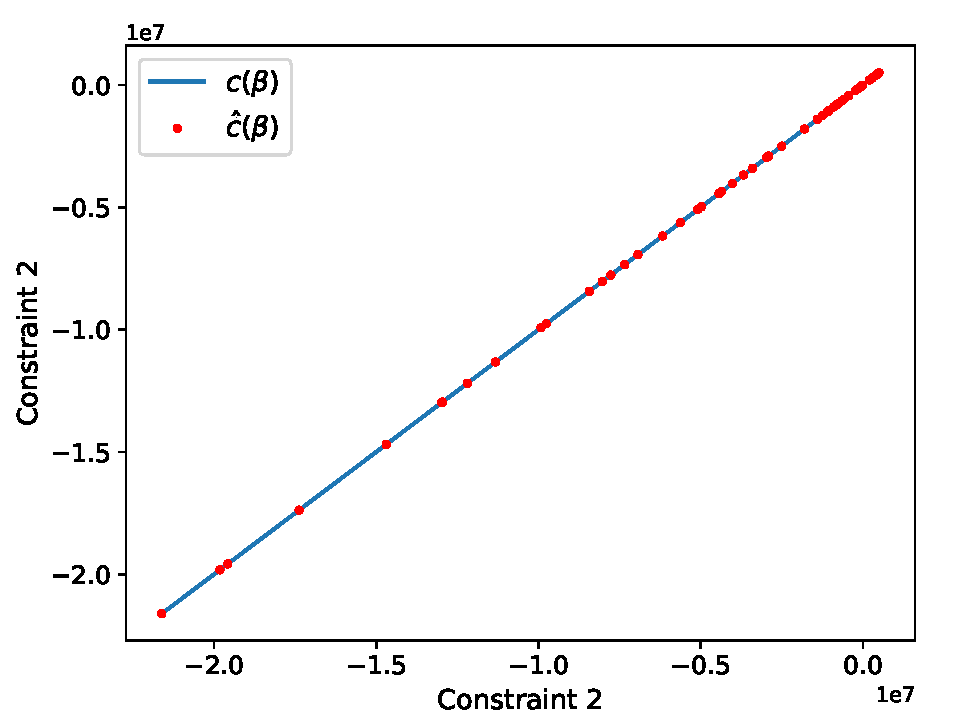
\includegraphics[width=\textwidth, height=0.58\textwidth, 
    scale=1]{welded_beam_con2_fitness_end.pdf}    
    \end{subfigure}
\caption{Case 3, welded beam case with RNG1. Deviation between 
exact $\mathrm{PSM}^{''}$ constraint values $\vec{c}(\vec{β})$ and 
Kriging predictions $\hat{\vec{c}}(\vec{β})$ given via the 
implementation of SMT. The initial Kriging model, which 
approximates the first two constraint functions, is trained on 
$n_{doe} \!= \!240$ and the final on $n_{doe}^{'} \!= \!429$ 
training patterns.}
\label{fig:fitting_con1_2_welded_beam}
\end{figure}

\newpage
%--------------------------------------------------------------

\begin{figure}[h!]
\centering
    \begin{subfigure}[b]{0.45\textwidth}
    \centering
    \caption{Initial $c_{3}$, $\mathrm{NRMSE} \!= \!0.00000008$}
    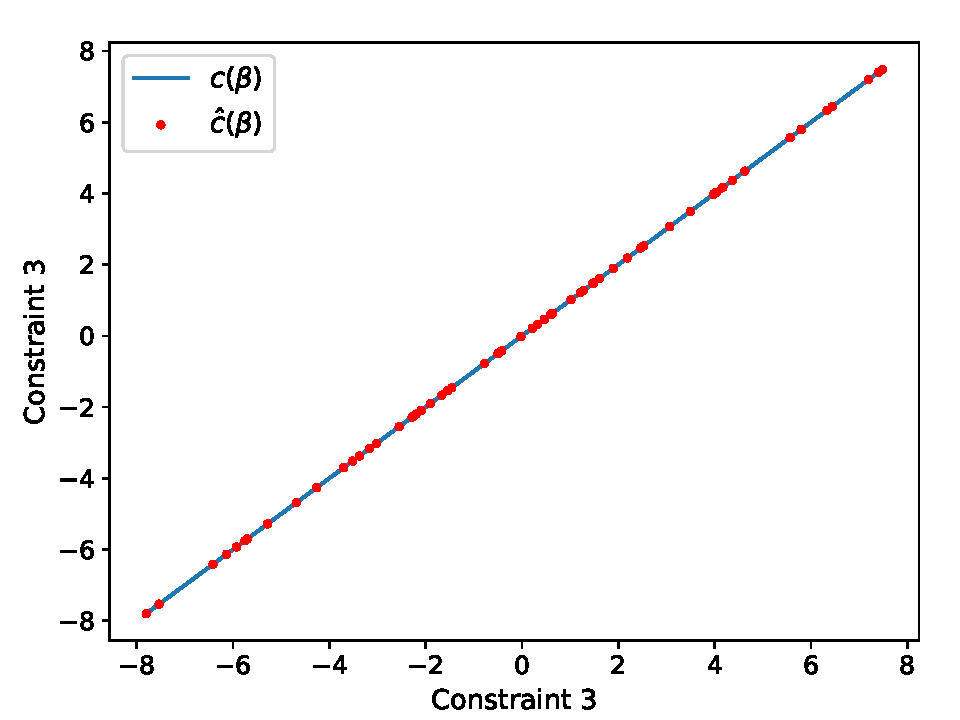
\includegraphics[width=\textwidth, height=0.6\textwidth, 
    scale=1]{welded_beam_con3_fitness_start.pdf}    
    \end{subfigure}
    \hfill
    \begin{subfigure}[b]{0.45\textwidth}
    \centering
    \caption{Final $c_{3}$, $\mathrm{NRMSE} \!= \!0.00000003$}
    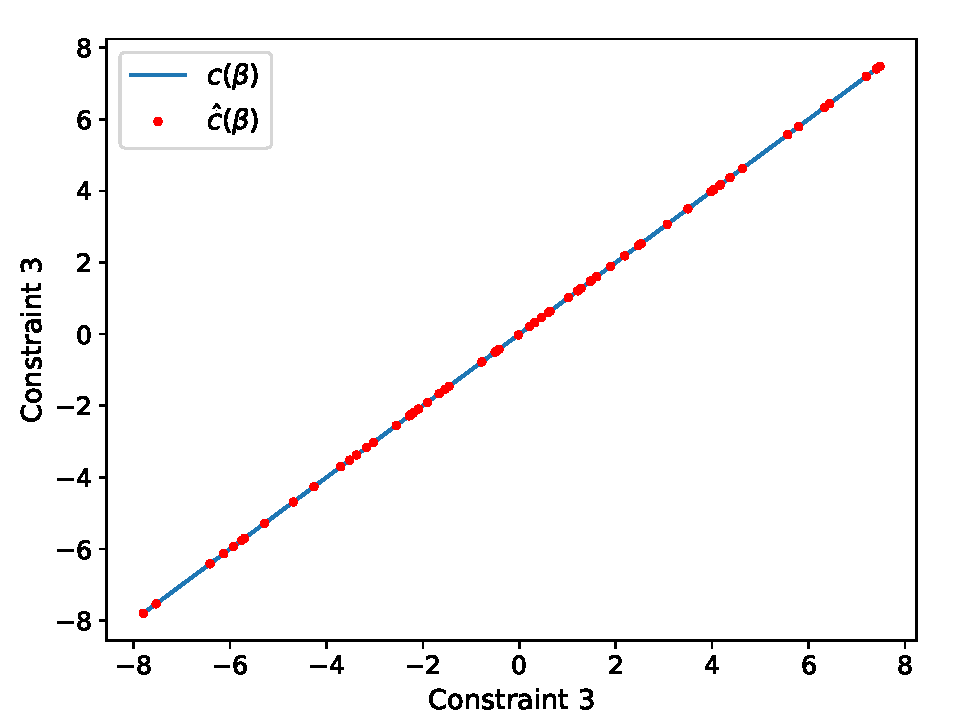
\includegraphics[width=\textwidth, height=0.6\textwidth, 
    scale=1]{welded_beam_con3_fitness_end.pdf}    
    \end{subfigure}
    \hfill
    \begin{subfigure}[b]{0.45\textwidth}
    \centering
    \caption{Initial $c_{4}$, $\mathrm{NRMSE} \!= \!0.00000617$}
    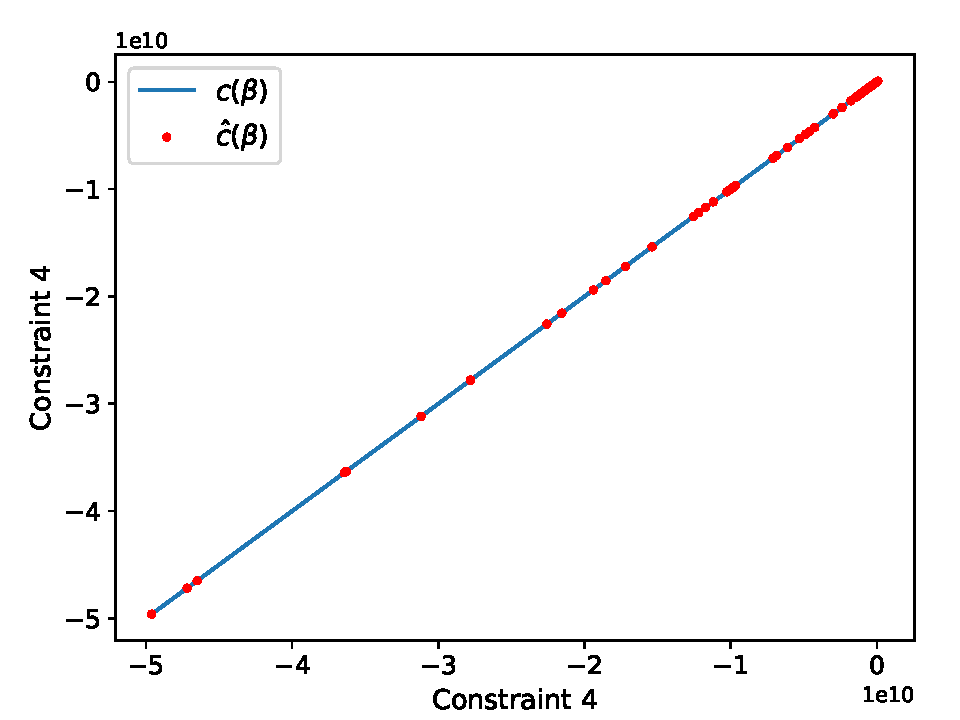
\includegraphics[width=\textwidth, height=0.6\textwidth, 
    scale=1]{welded_beam_con4_fitness_start.pdf}    
    \end{subfigure}
    \hfill
    \begin{subfigure}[b]{0.45\textwidth}
    \centering
    \caption{Initial $c_{4}$, $\mathrm{NRMSE} \!= \!0.00000131$}
    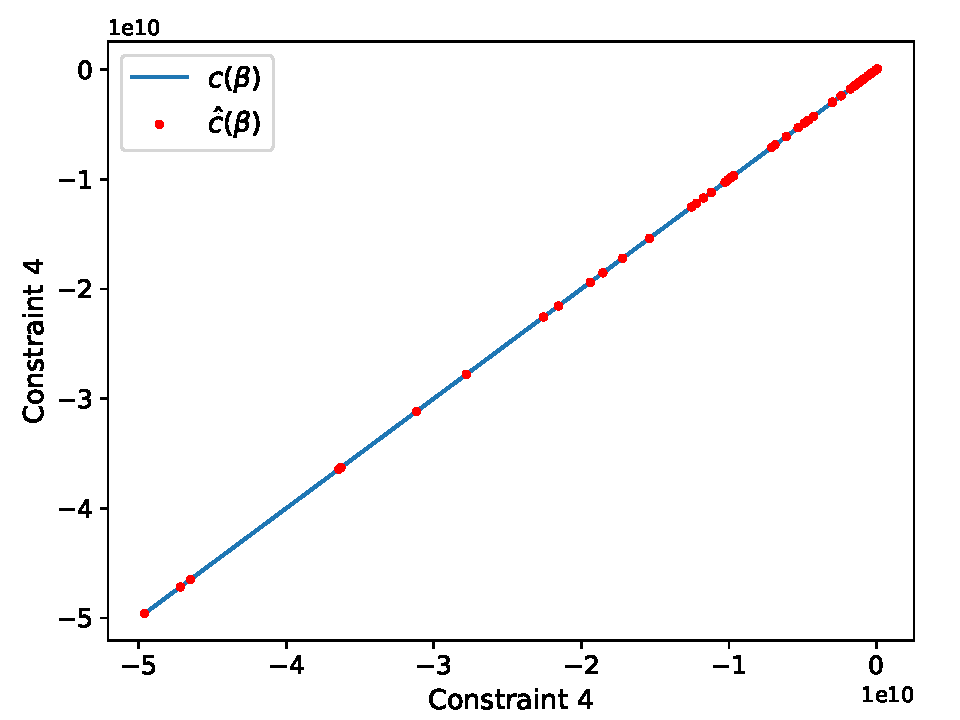
\includegraphics[width=\textwidth, height=0.6\textwidth, 
    scale=1]{welded_beam_con4_fitness_end.pdf}   
    \end{subfigure}
    \hfill
    \begin{subfigure}[b]{0.45\textwidth}
    \centering
    \caption{Final $c_{5}$, $\mathrm{NRMSE} \!= \!0.00000053$}
    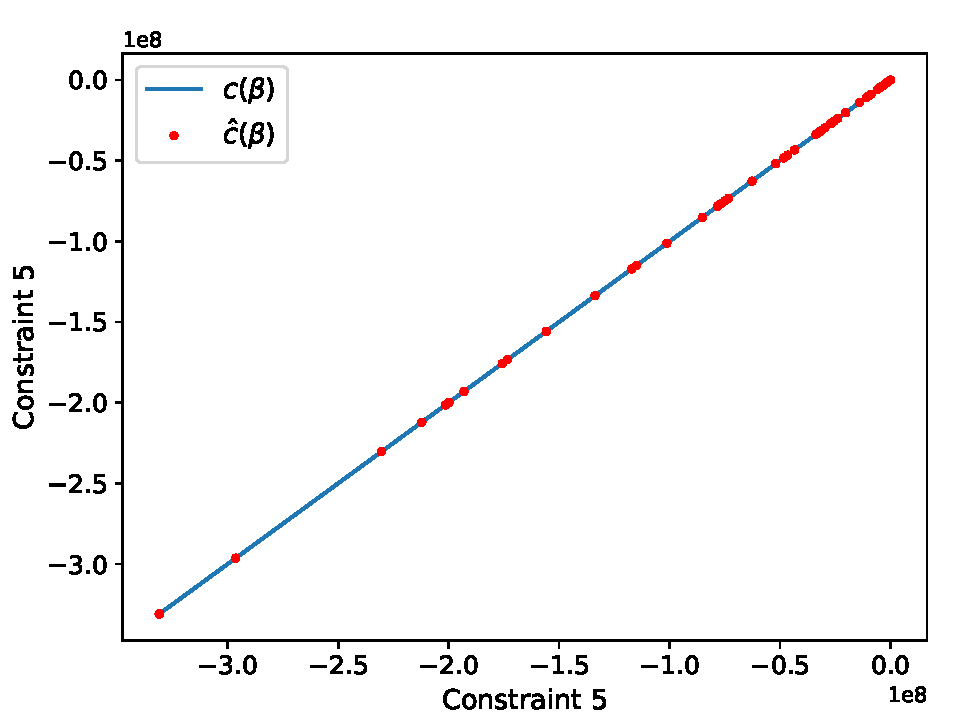
\includegraphics[width=\textwidth, height=0.6\textwidth, 
    scale=1]{welded_beam_con5_fitness_start.pdf}   
    \end{subfigure} 
    \hfill
    \begin{subfigure}[b]{0.45\textwidth}
    \centering
    \caption{Final $c_{5}$, $\mathrm{NRMSE} \!= \!0.00000014$}
    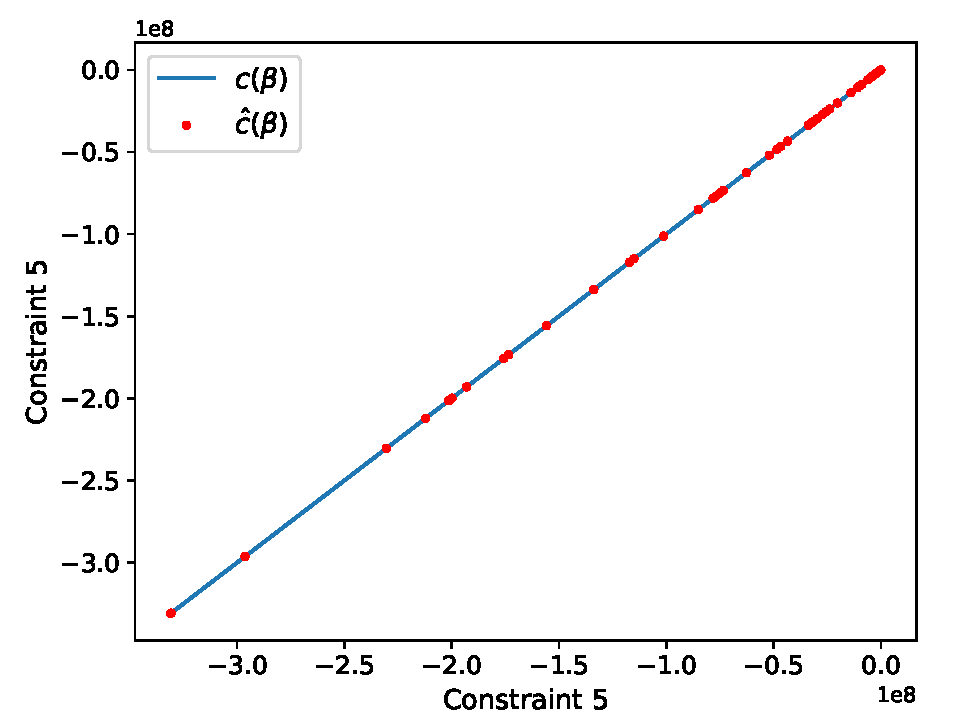
\includegraphics[width=\textwidth, height=0.6\textwidth, 
    scale=1]{welded_beam_con5_fitness_end.pdf}    
    \end{subfigure}
\caption{Case 3, welded beam case with RNG1. Deviation between 
exact PSM constraint values $\vec{c}(\vec{β})$ and RBF predictions 
$\hat{\vec{c}}(\vec{β})$ given via the implementation of SMT. The 
initial Kriging model, which approximates the remaining three 
constraint functions, is trained on $n_{doe} \!= \!240$ and the 
final on $n_{doe}^{'} \!= \!429$ training patterns.}
\label{fig:fitting_con3_5_welded_beam}
\end{figure}

The NRMSE calculates the mean normalised deviation between the 
predicted and exactly evaluated on the $\mathrm{PSM}^{''}$ values 
on $λ\!=\!60$ untried design sites $\mathbf{Β}$, where $\vec{β} 
\!= \!\vec{β}_{i} \!= \![β_{i,1}, β_{i,2}, \hdots, β_{i,n_{β}}] \in 
P_{λ}^{0}$ is any untried point in the design space contained in 
the initial offspring population set. NRMSE serves as a metric of 
model fitting and indicates that all trained metamodels are 
well-fitted, except from the one built on the 1st constraint 
function $c_{1}(\vec{β})$. This underfitted surrogate model hinders 
the convergence of the optimization process, which reaches an 
satisfactory optimal solution after 8 cycles. 

\newpage


%------------------------------------------------------------
%---------------On line----------------
%----------------------------------------------------------
\begin{itemize}
\item \textbf{Optimization using MAEAs with on-line trained 
matamodels}
\end{itemize}

In the MAEA-based optimization of welded beam design using on-line 
trained metamodels, the LCPE phase is set to initiate once 480 
exact evaluations are performed. In LCPE, personalised local
metamodels are trained on $20 \leq n_{t} \leq 21$ training 
patterns and subsequently  $2 \leq λ_{e} \leq 4$ individuals
are re-evaluated using the exact evaluation model. A total of 
10000 PSM evaluations are performed, unless 75
generations are formed without improving the current outcome, in 
which case the optimization terminates. Local metamodels are built 
by utilizing either the assisting software SMT or EASY. The former 
accommodates the use of Kriging, KPLS, KPLSK and RBFs, while the 
latter relies on Kriging and most often RBFs. In order to identify 
the most suitable metamodel in SMT for the welded beam 
optimization case, a comparison between each respective model 
is performed w.r.t. the convergence history and the produced 
outcome; the results of each comparison are presented in table 
figure \ref{fig:SMT_models_welded_beam} and table  
\ref{table:online_SMT_welded_beam}, respectively.  

\begin{figure}[h!]
\centering
	\begin{subfigure}[b]{0.49\textwidth}
	\centering
	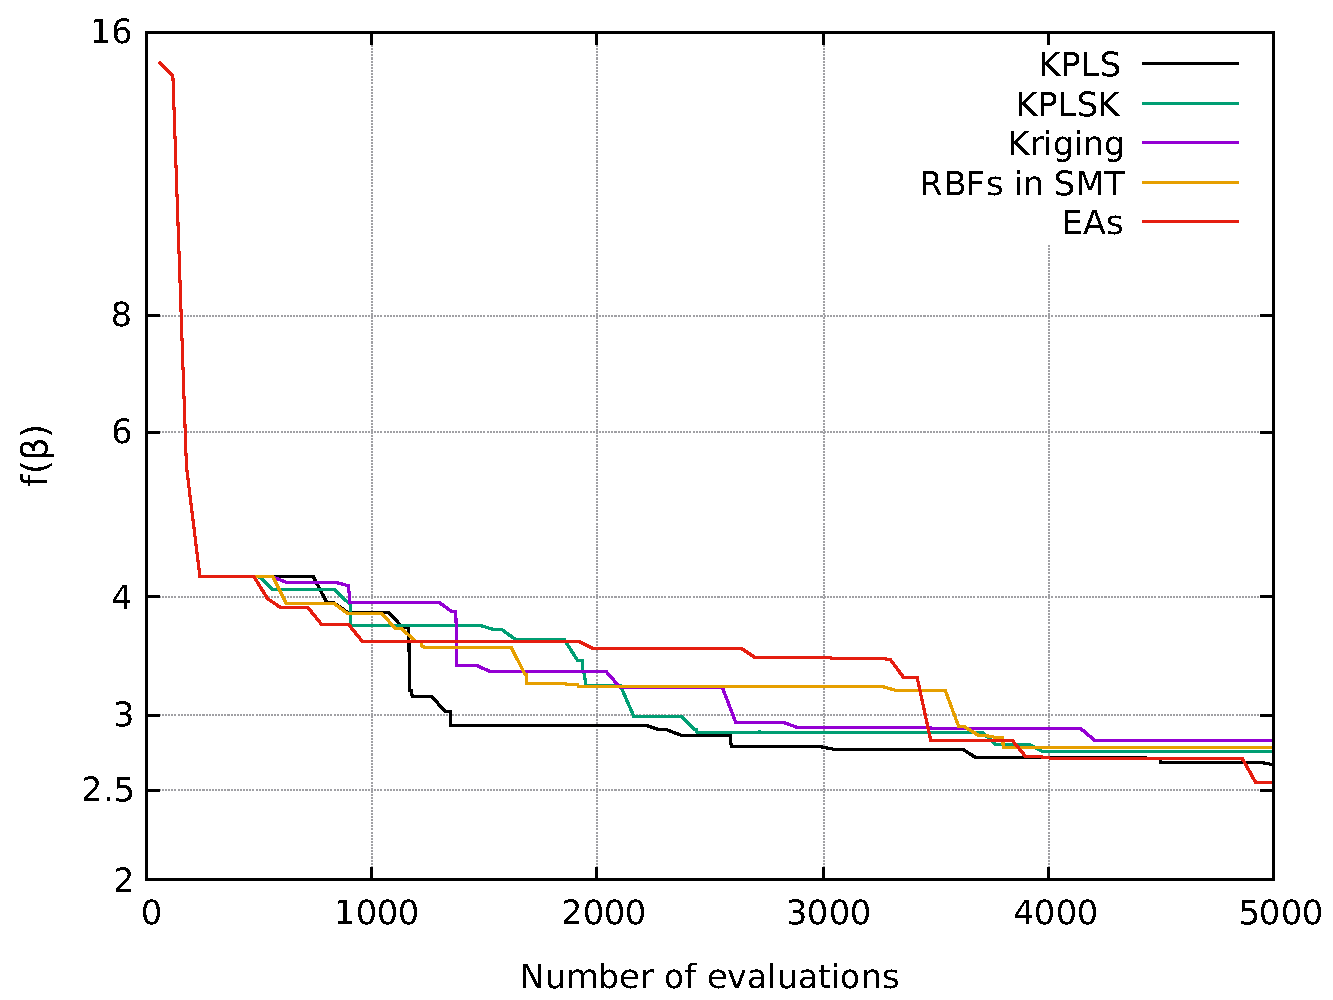
\includegraphics[width=\textwidth, height = 0.9\textwidth, 
	scale=1]{welded_beam_online_comparison.pdf}
	\end{subfigure}
	\hfill
	\begin{subfigure}[b]{0.49\textwidth}
	\centering
	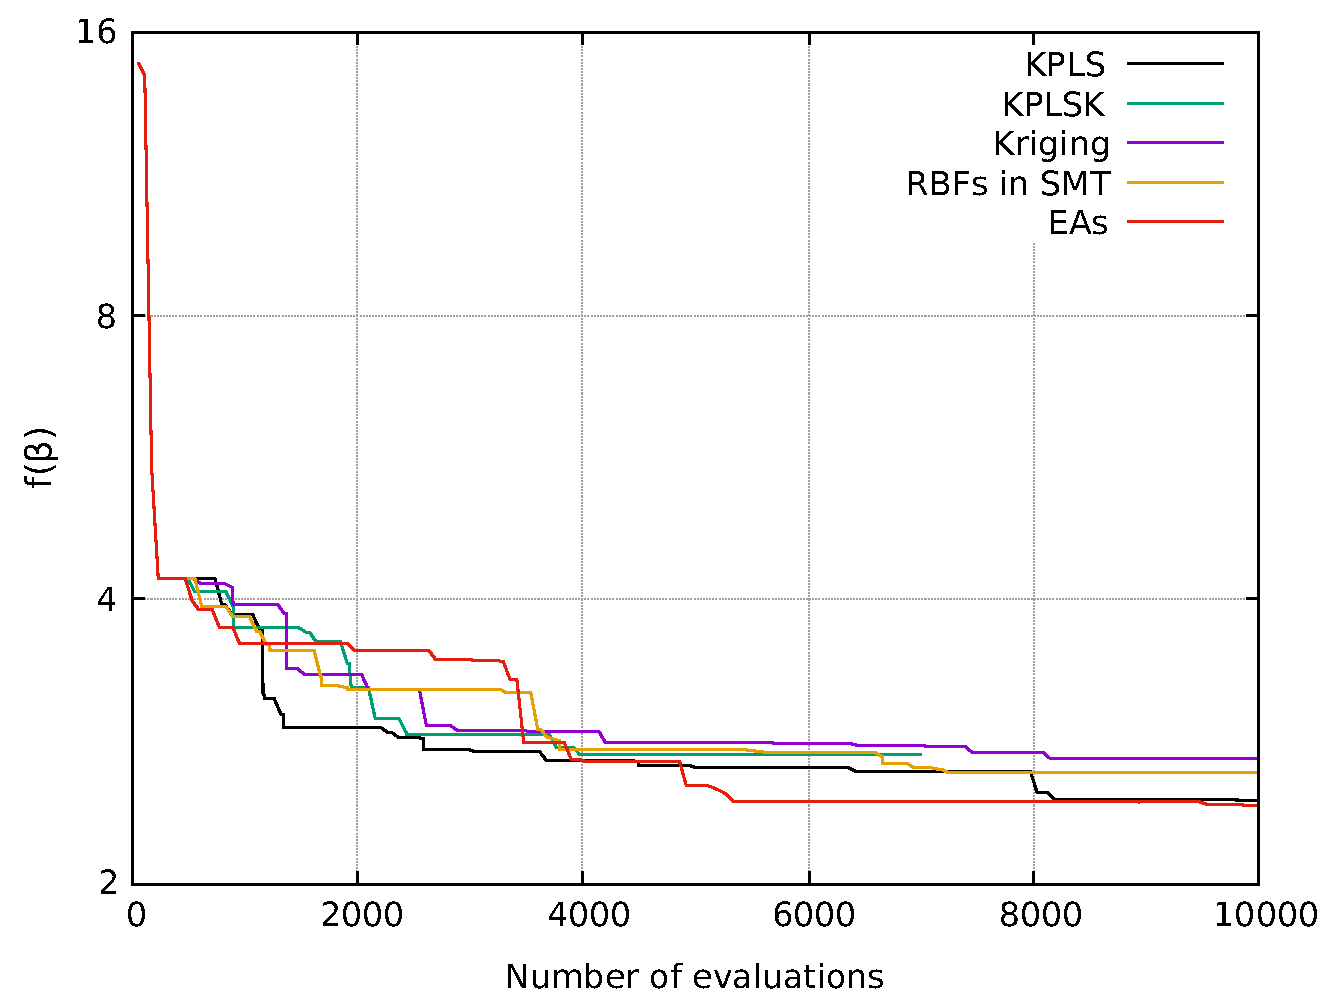
\includegraphics[width=\textwidth, height = 0.9\textwidth, 
	scale=1]{welded_beam_online_comparison2.pdf}
	\end{subfigure}   
\caption{Welded beam design with RNG1. Comparison between the 
convergence history of EAs and MAEAs with metamodels trained 
on-line via SMT} 
\label{fig:SMT_models_welded_beam}
\end{figure}

\begin{table}[h!]
\centering
%\rowcolors{2}{gray!30!}{white!50!gray!10}
\scalebox{0.83}{%
\begin{tabular}[c]{ |p{1.7cm}||p{1.6cm}|p{1.6cm}|p{1.6cm}|
p{1.6cm}|p{1.6cm}|}
\toprule
\multicolumn{6}{|c|}{\cellcolor{gray!30!} 
\textbf{Welded beam case}} \\
\midrule 
\textbf{MAEAs, on-line} & $(μ,λ)$ \textbf{population}  
& \textbf{KPLS} & \textbf{KPLSK} & \textbf{Kriging} 
& \textbf{RBFs} \\
\hline
\textbf{SMT} & (30, 100) & 2.45 & 2.74 & 2.72 & 2.62 \\
\bottomrule
\end{tabular}%
}
\caption{Welded beam case with RNG1. Optimal candidate solution 
found using metamodels trained on-line via SMT}
\label{table:online_SMT_welded_beam}
\end{table}

The comparison between convergence histories of the SMT built-in
metamodels, depicted in figure \ref{fig:SMT_models_welded_beam}, 
indicates that KPLS model is most suitable to facilitate the 
optimization of the welded beam case due to its fast convergence to 
the threshold of both 5000 and 10000 PSM evaluations. In plain EAs, 
RNG1 yields the best optimization outcome and for that reason MAEAs 
with on-line training are initialized with the same offspring 
population $P_{λ}^{0}$.

\newpage
%------------------------------------------------------------------


KPLS is yet to be compared to EASY built-in RBFs and plain EAs; 
the results are presented in table 
\ref{table:online_SMT_EASY_comparison_welded_beam}.
 
\begin{table}[h!]
\centering
%\rowcolors{2}{gray!30!}{white!50!gray!10}
\scalebox{0.87}{%
\begin{tabular}[c]{ |p{2.2cm}||p{1.5cm}|p{1.4cm}|p{1.4cm}|
p{1.8cm}|p{1.4cm}|p{2.4cm}|}
\toprule
\multicolumn{7}{|c|}{\cellcolor{gray!30!} 
\textbf{Welded beam design}} \\
\midrule 
\textbf{MAEAs, on-line} & $(μ,λ)$ \textbf{population} 
& \textbf{Best} & \textbf{Worst} & \textbf{Average} 
& \textbf{Avg. exact eval.} 
& \textbf{Avg. metamodel eval.}  \\
\hline
\textbf{SMT} & (20, 60) & 2.45 & 2.62 & 2.54 & 10000 & 11579 \\
\textbf{EASY} & (20, 60) & 2.38 & 2.82 & 2.53 & 10000 & 10738 \\
\hline
\textbf{Plain EAs} & (20, 60) & 2.42 & 3.05 & 2.59 & 10000 & - \\
\bottomrule
\end{tabular}%
}
\caption{Welded beam case. Comparison between the outcome of the  
optimization using MAEAs with on-line training and plain EAs}
\label{table:online_SMT_EASY_comparison_welded_beam}
\end{table}

The design variable vector that minimizes the construction
cost of the welded beam via the implementation of KLPS is $\vec{β} 
\!= \![0.234, 5.717, 9.276,$ $0.239]$. For MAEAs utilizing EASY 
built-in RBFs the respective optimal design variable vector is 
$\vec{β} = [0.255, 5.664, 8.527, 0.260]$.
 
\begin{figure}[h!]
\centering
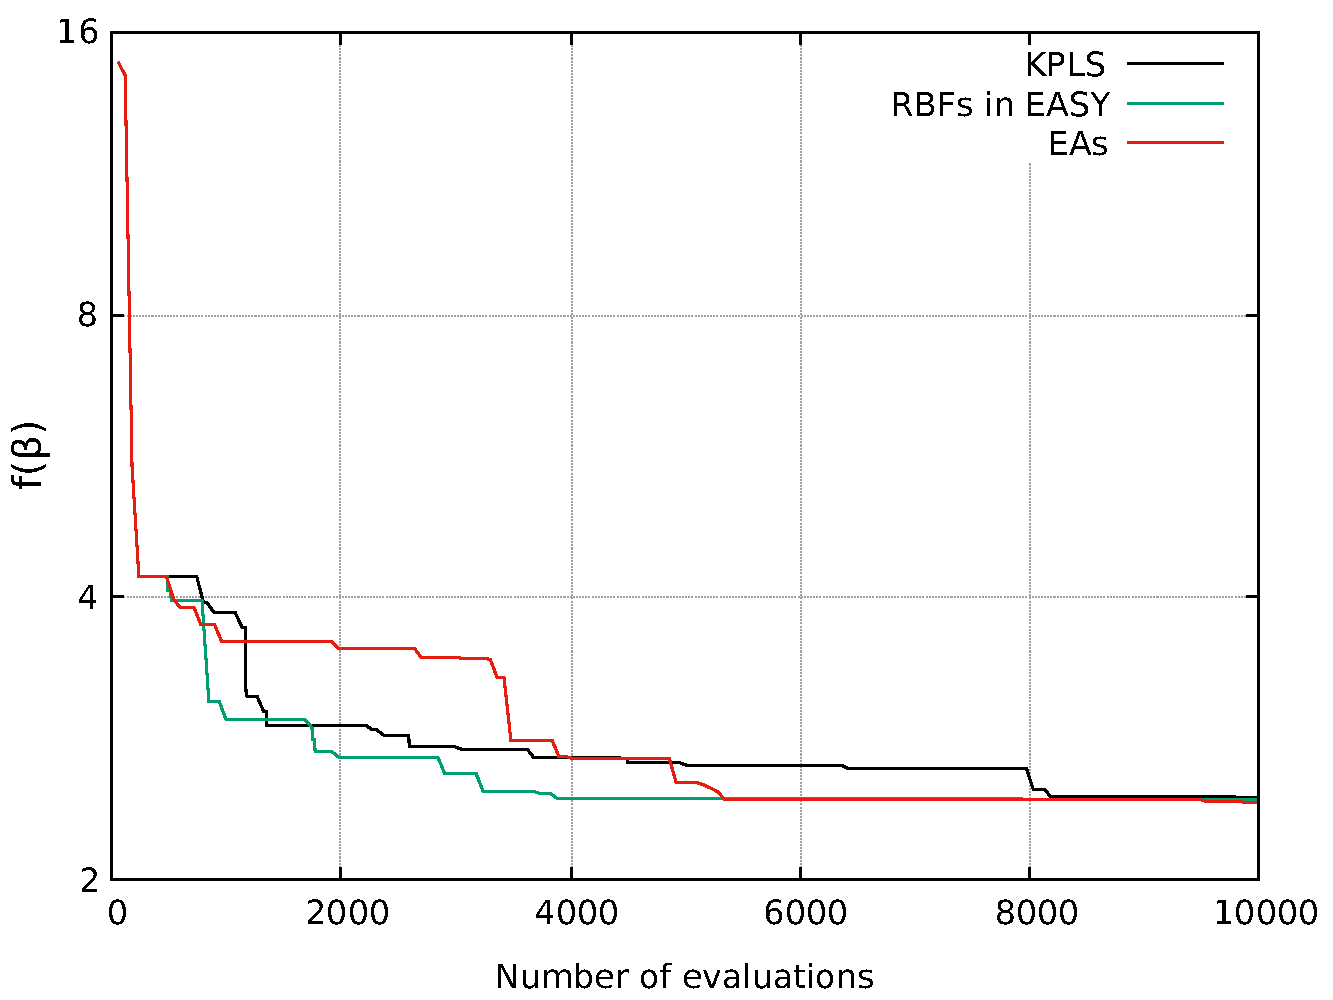
\includegraphics[width=0.68\textwidth, height=0.5\textwidth, 
scale=1]{welded_beam_online.pdf}   
\caption{Welded beam case with RNG1. Comparison between the 
convergence histories of the optimization using EAs and MAEAs 
with metamodels trained on-line via SMT and EASY} 
\label{fig:SMT_EASY_welded_beam}
\end{figure}

In the comparison of convergence histories depicted in figure 
\ref{fig:SMT_EASY_welded_beam}, EASY built-in RBFs are seemingly 
more accurate than KPLS model and yield a faster convergence. The 
impact of MAEAs on the computational cost is evident, since they 
outperform conventional EAs prior to the threshold of 10000 exact 
PSM evaluations.


\vfill

\newpage
%--------------------------------------------------------------


\subsection{MOO of Welded Beam Design}

The welded beam case appears in the majority of the scholar
literature as SOO problem, where the single objective is the 
minimization of the fabrication cost of the design. However, 
a variation of this optimization case also exists where the
welded beam design is optimized w.r.t. to two objectives, 
which are the fabrication cost of the design and the deflection 
$δ(\vec{β})$ of the beam. In this case, the deflection of the 
beam does not bound the design space of possible candidate 
solutions and the optimization problem assumes the following 
mathematical expression:
\begin{equation}
\begin{split}
min \hspace{2mm} & f_{1}(\vec{β}) = 1.10471β_{1}^{2}β_{2} + 
0.04811β_{3}β_{4}(14.0 + β_{2})
\\ &
f_{2}(\vec{β}) = \dfrac{2.1952}{β_{4}β_{3}^{3}} 
\\[0.3cm] 
\text{subject to} \hspace{2mm} & c_{1}(\vec{β}) = 
τ(\vec{β}) - τ_{max} \leq 0 
\\ &
c_{2}(\vec{β}) = σ(\vec{β}) - σ_{max} \leq 0
\\ &
c_{3}(\vec{β}) = β_{1} - β_{4} \leq 0
\\ &
c_{4}(\vec{β}) = P - P_{c}(\vec{β}) \leq 0
\end{split}
\end{equation}
\\[-2mm]
where the bounds of each design variable are $0.125 \leq 
β_{1} \leq 10.0$, $0.1 \leq β_{2} \leq 10.0$, $0.1 \leq β_{3} 
\leq 10.0$ and $0.1 \leq β_{4} \leq 10.0$. The formulas that 
describe $τ(\vec{β})$, $σ(\vec{β})$ and $P_{c}(\vec{β})$ can 
be found in equations \ref{welded_con1}, \ref{welded_con2} 
and \ref{welded_con5}, respectively. In this case, the 
objectives are conflicting and their corresponding values are 
presented in figure \ref{fig:Pareto_welded_beam}.

\begin{figure}[h!]
\centering
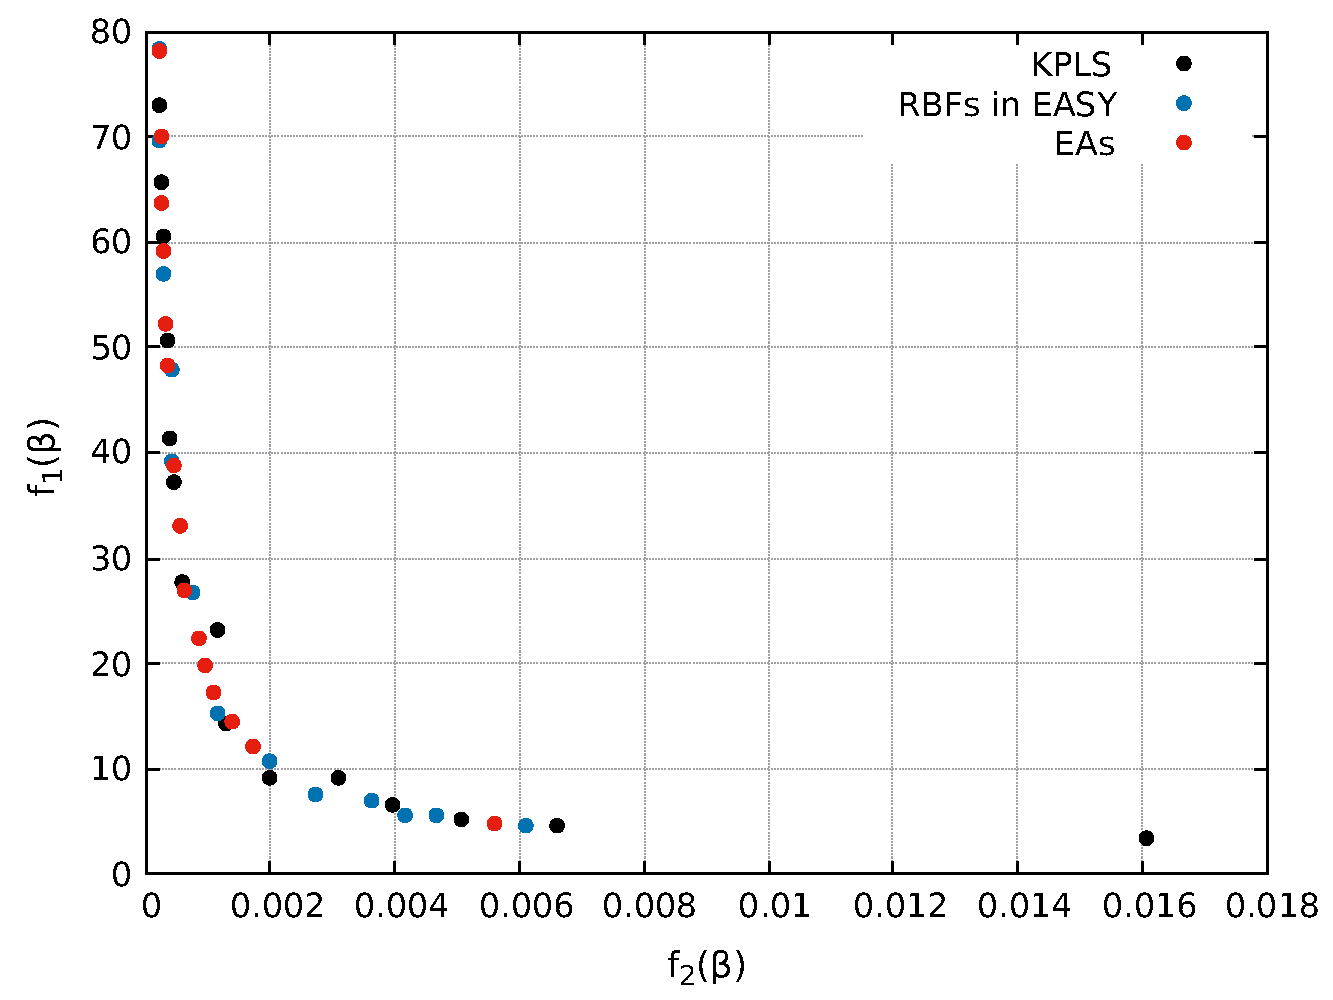
\includegraphics[width=0.57\textwidth]{pareto_welded_beam.pdf}
\caption{Pareto front of 15 non-dominated candidate solutions 
found in the MOO welded beam case for 1000 exact PSM evaluations} 
\label{fig:Pareto_welded_beam}
\end{figure}

The first two fronts are obtained by optimizing the MOO welded 
beam case via the use of MAEAs with on-line training, namely EASY 
built-in RBFs and the KPLS model found in SMT. The LCPE phase is 
set to initiate once 240 exact evaluations are performed on the 
PSM. In LCPE, personalised local metamodels are trained on $20 
\leq n_{t} \leq 21$ training patterns and subsequently  $2 \leq 
λ_{e} \leq 6$ individuals are re-evaluated using the exact 
evaluation model. The comparison is completed by the front that 
results from the optimization of the MOO case via the use of plain 
EAs. 

\newpage
%----------------------------------------------------------------


Since all fronts are seemingly overlapping, it is not evident 
which method yielded the best outcome. A way to determine this, 
is by calculating the hypervolume indicator \cite{hypervolume 
indicator} of each front $\mathcal{F} \subset \mathbb{R}^{n}$, 
which is defined as the measure of the region weakly dominated by 
$\mathcal{F}$ and bound by a reference point $\vec{x}_{r} \in 
\mathbb{R}^{n}$ and expressed as:

\begin{equation}
H(\mathcal{F}) = Λ \left( \{ \vec{p} \in \mathbb{R}^{n} | 
\hspace{1mm} \exists \vec{q} \in \mathcal{F}: \vec{q} \leq \vec{p} 
\hspace{2mm} \text{and} \hspace{2mm} \vec{p} \leq  \vec{x}_{r} \}
\right)
\end{equation} 
\\[-3mm]
where $H(\cdot)$ denotes the Lebesgue measure which is a way  
of assigning measure to subsets $\mathcal{F}$ of $n$-dimensional 
Euclidean space. In the 2D space, which is the case here, the 
Lebesgue measure $H(\mathcal{F})$ is equivalent to the area 
defined by each $\vec{q} \in \mathcal{F}$ and the reference point
$\vec{x}_{r} \in \mathbb{R}^{n}$. The coordinates ($x_{r_{1}}, 
x_{r_{2}}$) of the reference point in 2D space are defined as:
\begin{equation}
\begin{split}
& x_{r_{1}} \!= \! \{ q_{1} \in \mathcal{F}_{i}: q_{1} \geq ξ, 
\forall ξ \in \mathcal{F}_{i}, \forall i \in [1, n_{f}] \} + ξ_{1}
\\ &
x_{r_{2}}  \!= \! \{ q_{2} \in \mathcal{F}_{i}: q_{2} \geq ξ, 
\forall ξ \in \mathcal{F}_{i}, \forall i \in [1, n_{f}] \} + ξ_{2}
\end{split}
\end{equation}
\\[-2mm]
where $q_{1}, q_{2}$ are the coordinates of $\vec{q} \in 
\mathcal{F}$ point in 2D space, $n_{f}$ is the number of 
compared fronts and $ξ_{1}, ξ_{2}$ user-defined values. In this
case, the parameters assume the values $(ξ_{1}, ξ_{2}) = (0.002, 
20)$ and $(x_{r_{1}}, x_{r_{2}}) = (0.0181, 98.27)$ and 
yield the hypervolume indicators for each Pareto front shown in 
figure \ref{fig:hypervolume_welded_beam}.

\begin{figure}[h!]
\centering
	\begin{subfigure}[b]{0.45\textwidth}
	\centering
	\caption{KPLS, $H \!= \! 1.6222$ }
	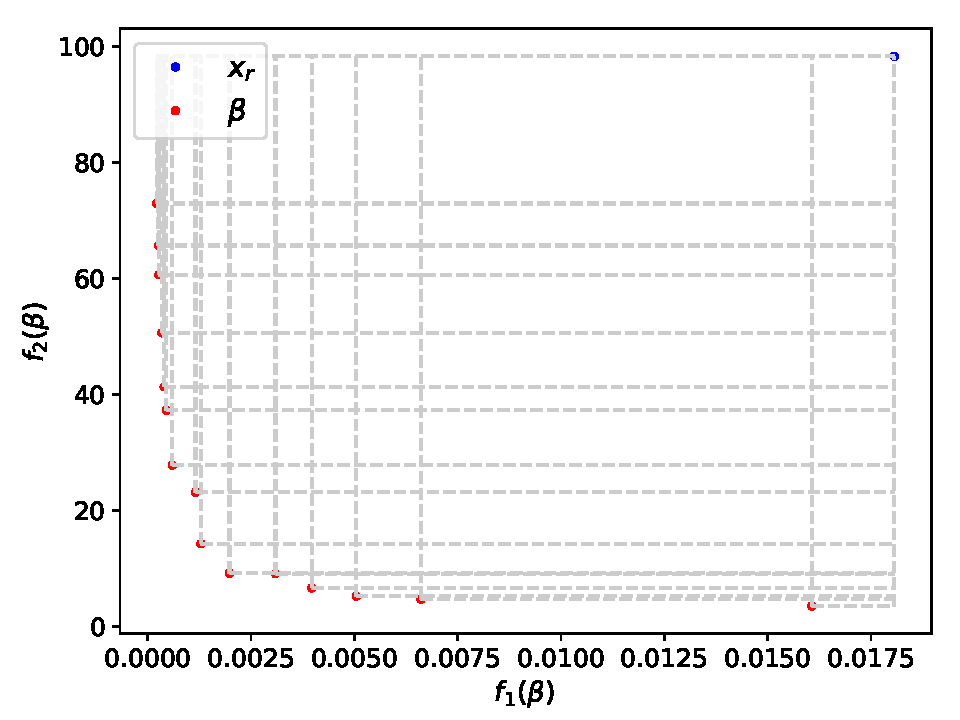
\includegraphics[width=\textwidth, height = 0.7\textwidth, 
	scale=1]{welded_beam_MOO_front1.pdf}
	\end{subfigure}
%--figure2
\hfill
	\begin{subfigure}[b]{0.45\textwidth}
	\centering
	\caption{RBFs in EASY, $H \!= \! 1.6215$ }
	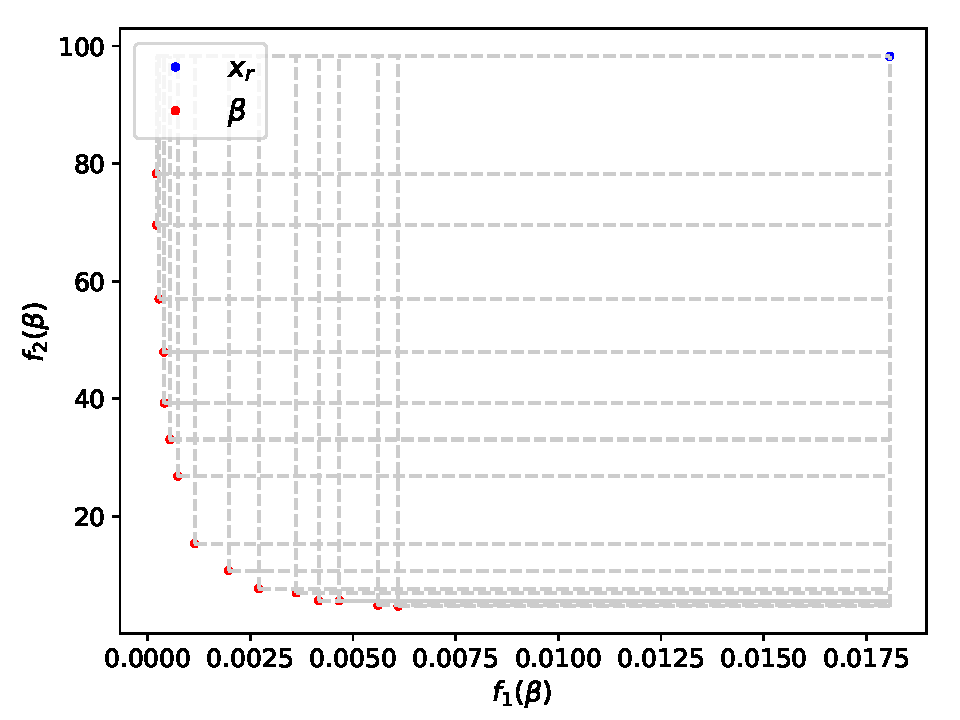
\includegraphics[width=\textwidth, height = 0.7\textwidth, 
	scale=1]{welded_beam_MOO_front2.pdf}
	\end{subfigure}
%-----figure3
\hfill
	\begin{subfigure}[b]{0.45\textwidth}
	\centering
	\caption{EAs, $H \!= \! 1.6061$ }
	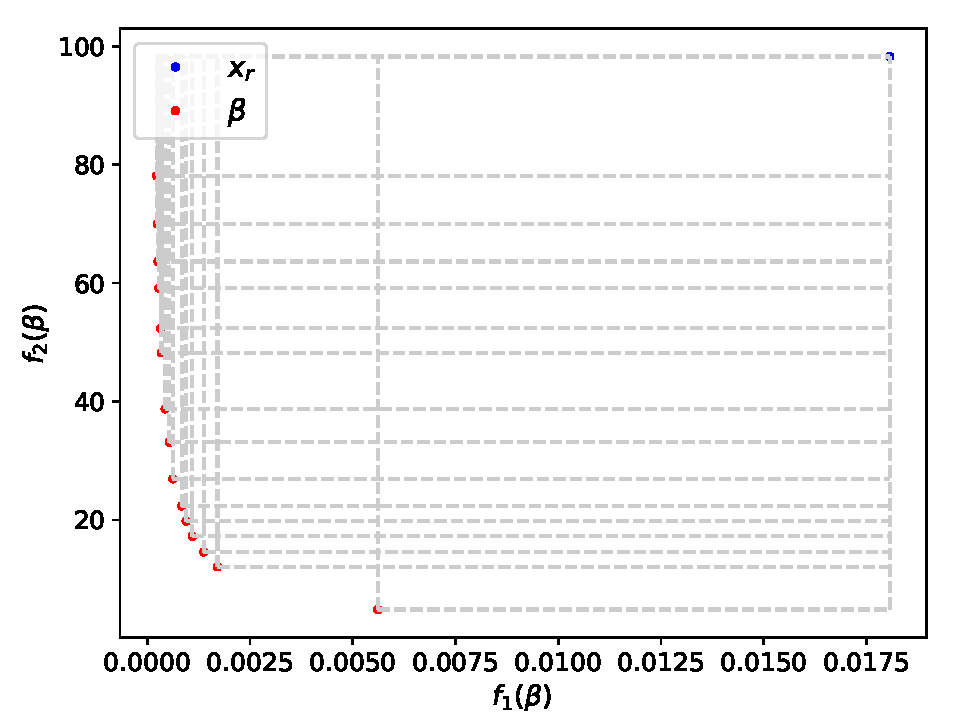
\includegraphics[width=\textwidth, height = 0.7\textwidth, 
	scale=1]{welded_beam_MOO_front3.pdf}
	\end{subfigure}
\caption{MOO welded beam case. Hypervolume indicator $H$ for 
fronts formed via the use of EAs, on-line trained KPLS and 
RBFs in EASY}
\label{fig:hypervolume_welded_beam}
\end{figure}

According to the $H$ value, the best front is the one formed via 
the use of on-line trained KPLS. Consequently, $\vec{β} = 
[0.481, 3.383, 6.572, 0.481]$ is selected that yields the response 
$(f_{1}, f_{2}) \!= \!(6.41, \hspace{1mm} 0.0031)$, since a 
minor increase in beam deflection yields a significant decrease in 
the fabrication cost.

\newpage
%---------------------------------------------------


\section{Speed Reducer Design}

The second optimization case is the SOO problem of minimizing
the overall weight of a speed reducer. This design is used to 
reduce the output speed by increasing the output torque via
the use two gears that are mounted to two separate shafts of
diameter $d_{1}$ and $d_{2}$. The structure is enclosed 
within a housing, while a pair of pairings is used at the 
connection point of each shaft in order to reduce friction 
produced by the rotation movement of the shafts (see figure 
\ref{fig:speed_reducer_image}). The minimization of the overall 
weight of the structure is, therefore, refers to the minimization 
of the total weight of both gears and shafts. The speed reducer 
case\cite{Golinski} is optimized w.r.t. the following design 
variables:

\begin{itemize}
\item Face width of the gear $b$ in [cm], 
where $2.6 \leq β_{1} \leq 3.6$ 
\item Teeth module $m$ in [cm], where $0.7\leq β_{2}\leq 0.8$
\item Number of pining teeth $N_{teeth}$,
where $17 \leq β_{3} \leq 28$
\item Length between bearings of the first shaft $L_{1}$ in 
[cm], where $7.3 \leq β_{4} \leq 8.3$ 
\item Length between bearings of the second shaft $L_{2}$ in 
[cm], where $7.3 \leq β_{5} \leq 8.3$ 
\item Diameter of the first shaft $d_{1}$ in [cm],
where $2.9 \leq β_{6} \leq 3.9$ 
\item Diameter of the second shaft $d_{2}$ in [cm],
where $5.0 \leq β_{7} \leq 5.5$ 
\end{itemize}

\begin{figure}[h!]
\centering
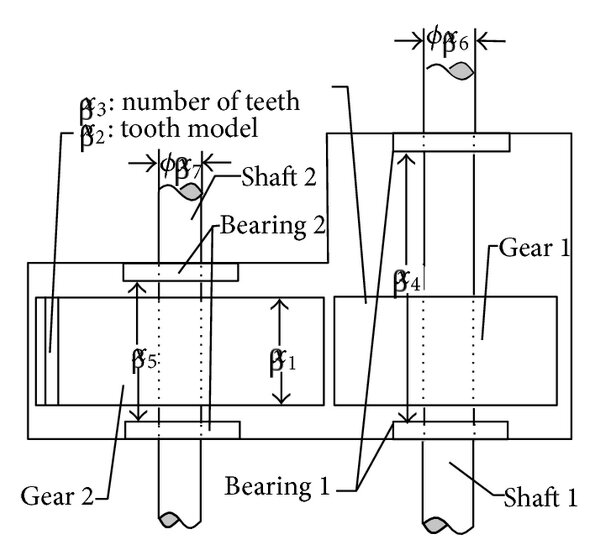
\includegraphics[width=0.6\textwidth]{speed_reducer}   
\caption{Speed reducer design} 
\label{fig:speed_reducer_image}
\end{figure}

\newpage
%----------------------------------------------------------


The volume of the speed reducer in [$cm^{3}$] can be 
calculated using the following equation \cite{speed reducer}, 
which multiplied by the density of the material yields the 
weight of the speed reducer:
\begin{equation}
\begin{split}
W_{spr} = \hspace{2mm} &  c_{1}bm^{2} \left( c_{2} 
N_{teeth}^{2} + c_{3} N_{teeth} - c_{4} \right) - c_{5}
\left( d_{1}^{\hspace{1mm}2} + d_{2}^{\hspace{1mm}2} \right) 
\\ &
c_{6} \left( d_{1}^{\hspace{1mm}3} + d_{2}^{\hspace{1mm}3} 
\right) + c_{1} \left( L_{1}d_{1}^{\hspace{1mm}2} 
+ L_{2}d_{2}^{\hspace{1mm}2} \right)
\end{split} 
\end{equation}

where the occurring parameters are calculated by Golinski 
\cite{Golinski}:
\begin{itemize}
\item $c_{1} = 0.7854$
\item $c_{2} = 3.3333$
\item $c_{3} = 14.9334$
\item $c_{4} = 43.0934$
\item $c_{5} = 1.508$
\item $c_{6} = 7.4777$
\end{itemize} 
\vspace{3mm}
and thus the previous equation can be restated as such:
\begin{equation}
\begin{split}
W_{spr} = \hspace{2mm} &  0.7854bm^{2} \left( 3.3333 
N_{teeth}^{2} + 14.9334 N_{teeth} - 43.0934 \right) - 1.508
\left( d_{1}^{\hspace{1mm}2} + d_{2}^{\hspace{1mm}2} \right) 
\\ &
7.4777 \left( d_{1}^{\hspace{1mm}3} + d_{2}^{\hspace{1mm}3} 
\right) + 0.7854 \left( L_{1}d_{1}^{\hspace{1mm}2} 
+ L_{2}d_{2}^{\hspace{1mm}2} \right)
\end{split} 
\end{equation}

The volume function is optimized in $\mathbb{R}^{7}$ space	
formed by the design variables $\{ b, m, N_{teeth}, L_{1}, 
L_{2}, d_{1}, d_{2} \}$. The design space is bound by the 
imposed constraints that are associated with limitations on 
the bending stress of gear teeth, surface stresses, transverse 
deflections of the shafts due to transmitted force and 
stresses in shafts. Subsequently the imposed constraints are
presented analytically. The upper bound on the bending stress 
of a gear tooth is given by the following formula:
\begin{equation}
σ_{g} = \dfrac{2M_{g}}{Ybm^{2}N_{teeth}} \leq σ_{g_{max}} 
\Rightarrow 
\dfrac{27}{bm^{2} N_{teeth}} \leq 1
\end{equation}
\\
where $Y = 0.3937$ is the Lewis tooth form factor, $M_{g}$
the bending moment for the gear teeth and $σ_{g_{max}} = 900 
\hspace{2mm} g/cm^{2}$ is the maximum bending stress of the 
gear teeth. Similarly the upper bound of the compressive stress of 
a gear tooth for both gears is defined as such:
\begin{equation}
P_{g_{1,2}} = \dfrac{2BM_{g}}{bm^{2}N_{teeth}^{2}} \leq  
P_{g_{max1,2}} \Rightarrow
\dfrac{397.5}{bm^{2}N_{teeth}^{2}} \leq 1
\end{equation}
\\
where $P_{g_{max1,2}} = 5800 \hspace{2mm} g/cm^{2}$ is the 
maximum surface compressive stress for both gears and $B$ is 
a coefficient dependent on Young's modulus of elasticity $E$.
\newpage
%----------------------------------------------------------


The transverse deflections of the shafts due to the 
transmitted load $P$ are required to not exceed the following
bounds:
\begin{equation}
\text{Shaft 1:} \hspace{5mm} 
δ_{1} = \dfrac{1}{48} \dfrac{PL_{1}^{2}}{EI_{1}} \leq δ_{1max}
\Rightarrow
\dfrac{1.93L_{1}^{3}}{mN_{teeth}
d_{1}^{\hspace{1mm}4}} \leq 1
\end{equation}

\begin{equation}
\text{Shaft 2:} \hspace{5mm}
δ_{2} = \dfrac{1}{48} \dfrac{PL_{2}^{2}}{EI_{2}} \leq δ_{2max}
\Rightarrow
\dfrac{1.93L_{2}^{3}}{mN_{teeth}
d_{2}^{\hspace{1mm}4}} \leq 1
\end{equation}
\\
where $I$ is the moment of inertia of the shafts and 
$δ_{1max}, δ_{2max}$ the maximum permissible transverse 
deflections of shaft 1 and 2 respectively.
\\
Subsequently, the bending stress conditions for the shafts are 
limited based on the following formulas:
\begin{equation}
\text{Shaft 1:} \hspace{5mm}
σ_{g_{1}} =  \dfrac{M_{z_{1}}}{W_{x_{1}}} \leq σ_{g_{1max}}
\Rightarrow
\dfrac{\sqrt{ \left( \dfrac{745L_{1}}{mN_{teeth}} \right)^{2} 
+ 16.9 \times 10^{6} }}{0.1d_{1}^{\hspace{1mm}3}} \leq 1100
\end{equation}

\begin{equation}
\text{Shaft 2:} \hspace{5mm} 
σ_{g_{2}} =  \dfrac{M_{z_{2}}}{W_{x_{2}}} \leq σ_{g_{2max}}
\Rightarrow
\dfrac{\sqrt{ \left( \dfrac{745L_{2}}{mN_{teeth}} \right)^{2} 
+  157.5 \times 10^{6} }}{0.1d_{2}^{\hspace{1mm}3}} \leq 850
\end{equation}
\\
where $σ_{g_{1max}} = 1100 \hspace{2mm} g/cm^{2}$, 
$σ_{g_{2max}} = 850 \hspace{2mm} g/cm^{2}$ are the maximum
permissible bending stresses for shaft 1 and 2, respectively.
$W_{x}$ is strength section modulus if each shaft and $M_{z}$
is moment of each shaft formulated by the equation:

$$ M_{z} = \sqrt{M_{g}^{2} + 0.75M_{s}^{2}} $$
\\[-0.2cm]
where $M_{s}$ is the torsional moment of each shaft.
\\
In order to improve the optimization process, various 
dimensional restrictions are applied based on experience:

\begin{equation}
i) \hspace{2mm}	\dfrac{mN_{teeth}}{40} \leq 1 \hspace{10mm} 
ii) \hspace{2mm} \dfrac{5m}{b} \leq 1 \hspace{10mm}
iii) \hspace{2mm} \dfrac{b}{12m} \leq 1
\end{equation}
\\
Similarly a pair of restrictions are applied on the dimensions 
of shafts based on previous experience:
\begin{equation}
\begin{split}
& 1.5d_{1} + 1.9 \leq L_{1}
\\ &
1.1d_{2} + 1.9 \leq L_{2}
\end{split}
\end{equation}  

\newpage
%-------------------------------------------------------


The final optimization case is formulated as such:
\begin{equation}
\begin{split}
min \hspace{2mm} f(\vec{β}) = \hspace{2mm} & 
0.7854bm^{2} \left( 3.3333 N_{teeth}^{2} + 14.9334 N_{teeth} 
- 43.0934 \right) - 1.508\left( d_{1}^{\hspace{1mm}2} + 
d_{2}^{\hspace{1mm}2} \right) 
\\ &
7.4777 \left( d_{1}^{\hspace{1mm}3} + d_{2}^{\hspace{1mm}3} 
\right) + 0.7854 \left( L_{1}d_{1}^{\hspace{1mm}2} 
+ L_{2}d_{2}^{\hspace{1mm}2} \right)
\\[0.4cm]
\text{subject to} \hspace{2mm} & c_{1}(\vec{β}) = 
\dfrac{27}{β_{1}β_{2}^{\hspace{1mm}2} β_{3}} -1 \leq 0
\\[0.3cm] &
c_{2}(\vec{β}) = \dfrac{397.5}{β_{1}β_{2}^{\hspace{1mm}2} 
β_{3}^{\hspace{1mm}2}} - 1 
\leq 0
\\[0.3cm] &
c_{3}(\vec{β}) = \dfrac{1.93β_{4}^{\hspace{1mm}3}}{β_{2}β_{3}
β_{6}^{\hspace{1mm}4}} - 1 \leq 0
\\[0.3cm] &
c_{4}(\vec{β}) = \dfrac{1.93β_{5}^{\hspace{1mm}3}}{β_{2}β_{3}
d_{7}^{\hspace{1mm}4}} - 1 \leq 0
\\[0.3cm] &
c_{5}(\vec{β}) = \dfrac{\sqrt{ \left( \dfrac{ 745β_{4} }{β_{2}
β_{3}} \right)^{2} + 
16.9 \times 10^{6} }}{110β_{6}^{\hspace{1mm}3}} - 1 \leq 0
\\[0.3cm] &
c_{6}(\vec{β}) = \dfrac{\sqrt{ \left( \dfrac{ 745β_{5} }{β_{2}
β_{3}} \right)^{2} 
+ 16.9 \times 10^{6} }}{85β_{7}^{\hspace{1mm}3}} - 1 \leq 0
\\[0.3cm] &
c_{7}(\vec{β}) = \dfrac{β_{2}β_{3}}{40} - 1 \leq 0
\\[0.3cm] &
c_{8}(\vec{β}) = \dfrac{5β_{2}}{β_{1}} - 1 \leq 0
\\[0.3cm] &
c_{9}(\vec{β}) = \dfrac{β_{1}}{12β_{2}} - 1 \leq 0
\\[0.3cm] &
c_{10}(\vec{β}) = \dfrac{1.5β_{6} + 1.9}{β_{4}} - 1 \leq 0
 \\[0.3cm] &
c_{11}(\vec{β}) = \dfrac{1.5β_{7} + 1.9}{β_{5}} - 1 \leq 0
\end{split}
\end{equation}

where the bounds of each design variable are $2.6 \leq β_{1} \leq 
3.6$, $\hspace{1mm} 0.7\leq β_{2}\leq 0.8$, $17 \leq β_{3} \leq 
28$, $\hspace{1mm} 7.3 \leq β_{4} \leq 8.3$, $\hspace{1mm} 7.3 
\leq β_{5} \leq 8.3$, $\hspace{1mm} 2.9 \leq β_{6} \leq 
3.9$, and $5.0 \leq β_{7} \leq 5.5$

\newpage
%-------EAs----------
%------------------------------------------------------
\begin{itemize}
\item \textbf{Optimization using EAs}
\end{itemize}

The optimization of the speed reducer design is performed via the 
use of plain EAs that utilize the PSM. Multiple experiments 
concluded that the optimal number of offspring and parent 
population is $(μ,λ) = (30, 100)$ where 5 parents are combined to 
create a single offspring with two-point crossover. Gray binary 
encoding is used where 12 bits are assigned to each design 
variable, except for $β_{2}, β_{3}$ and $β_{7}$ that are assigned 
8, 8 and 11 bits respectively. The optimization process terminates 
after 52000 total PSM evaluations have been performed 
and is repeated for 5 randomly initialised offspring populations 
$P_{λ}^{0}$ via the use of a RNG. The results are presented in
in table \ref{table:EAs_speed_reducer} and figure 
\ref{fig:EAs_speed_reducer}.
\begin{table}[h!]
\centering
%\rowcolors{2}{gray!30!}{white!50!gray!10}
\scalebox{0.84}{%
\begin{tabular}[c]{ |p{1.3cm}||p{1.6cm}|p{1.4cm}|p{1.4cm}|
p{1.8cm}|p{1.6cm}|p{1.6cm}| }
\toprule
\multicolumn{7}{|c|}{\cellcolor{gray!30!} 
\textbf{Speed reducer design}} \\
\midrule 
& $(μ,λ)$ \textbf{population} & \textbf{Best} & 
\textbf{Worst} & \textbf{Average} & \textbf{Exact model eval.} 
& \textbf{Average exact eval.} \\
\hline
\textbf{EAs} & (30, 100) & 2994.91 & 3001.97 & 2997.74 
& 52207 & 40246 \\
\bottomrule
\end{tabular}%
}
\caption{Optimization of speed reducer design using EAs}
\label{table:EAs_speed_reducer}
\end{table}

\vspace{-3mm}

\begin{figure}[h!]
\centering
	\begin{subfigure}[b]{0.47\textwidth}
    \centering
    \caption{Comparison between the convergence histories of 5 
    different $P_{λ}^{0}$ initializations}
    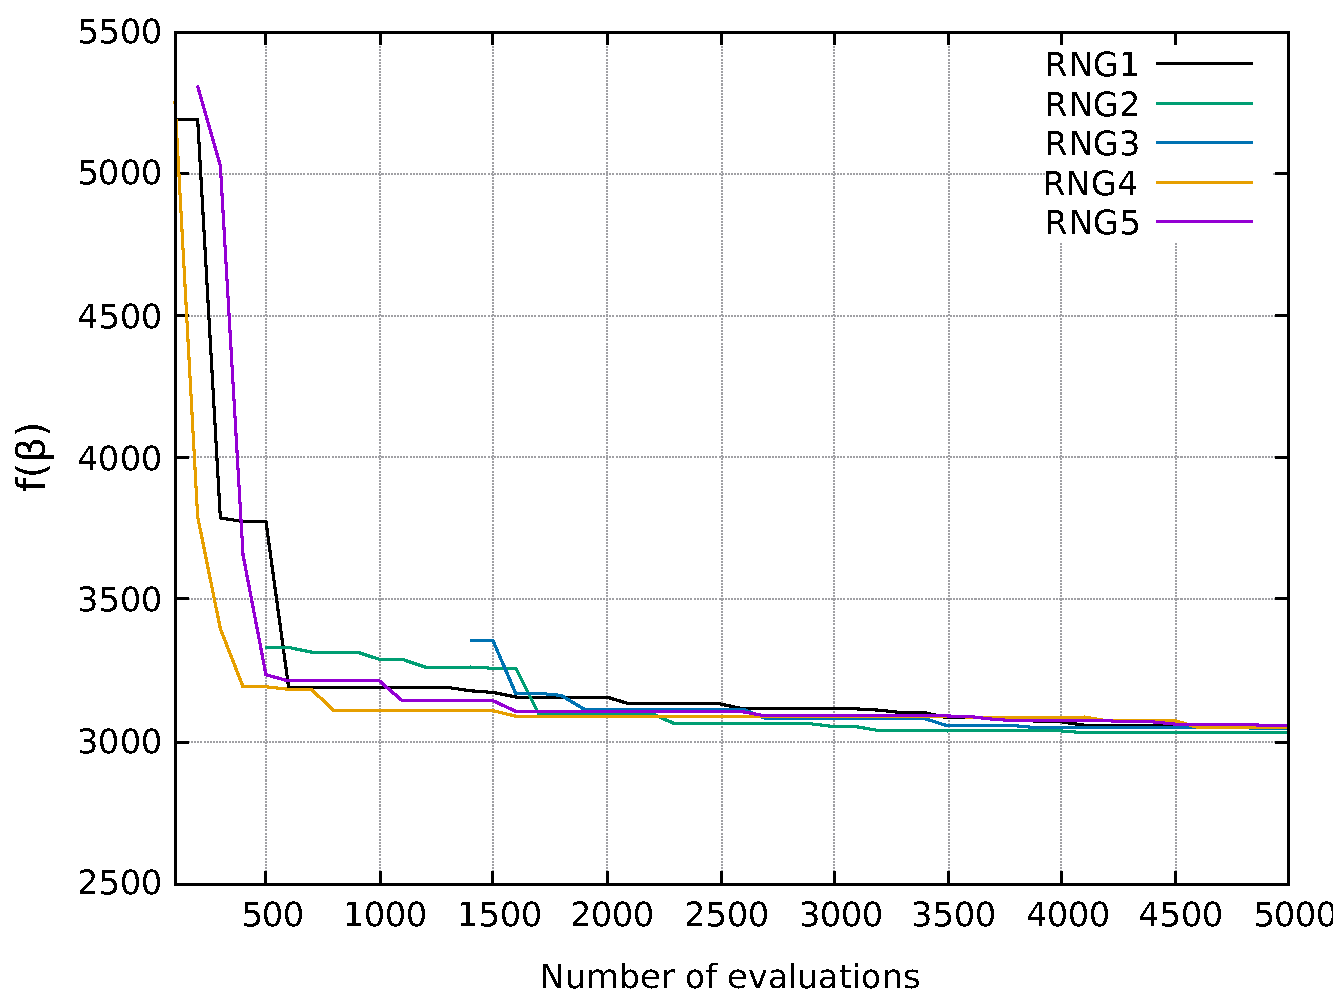
\includegraphics[width=\textwidth]{speed_reducer_ea1.pdf}    
    \end{subfigure}
    \hfill
    \begin{subfigure}[b]{0.47\textwidth}
    \centering
    \caption{Comparison between the convergence histories if 
    $f(\vec{β})$ range is narrowed}
    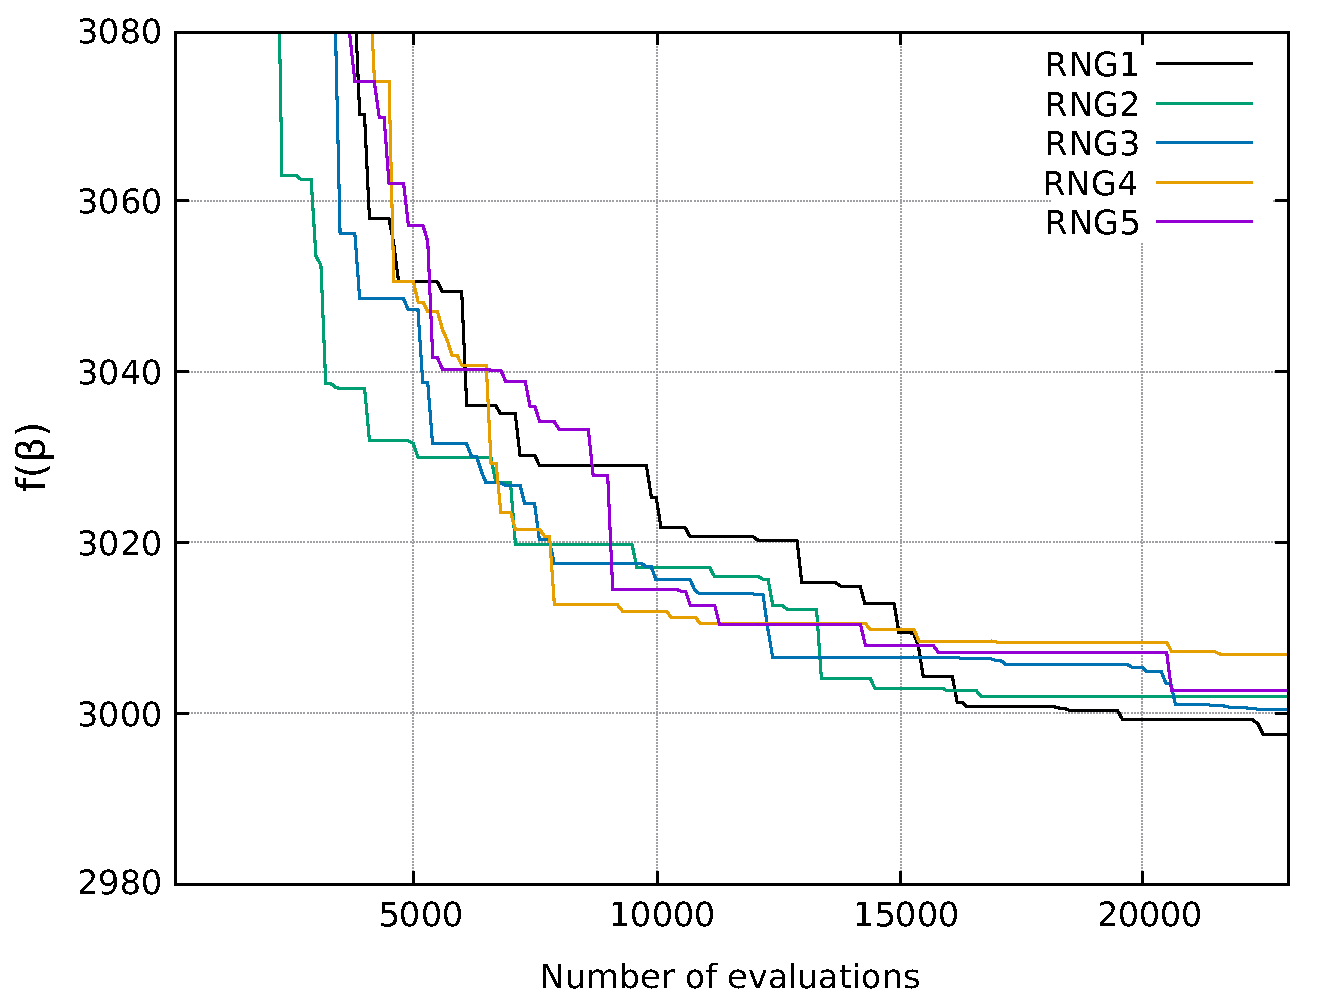
\includegraphics[width=\textwidth]{speed_reducer_ea2.pdf}    
    \end{subfigure}  
    \hfill
    \begin{subfigure}[b]{0.47\textwidth}
    \centering
    \caption{Convergence history of the optimal run}
    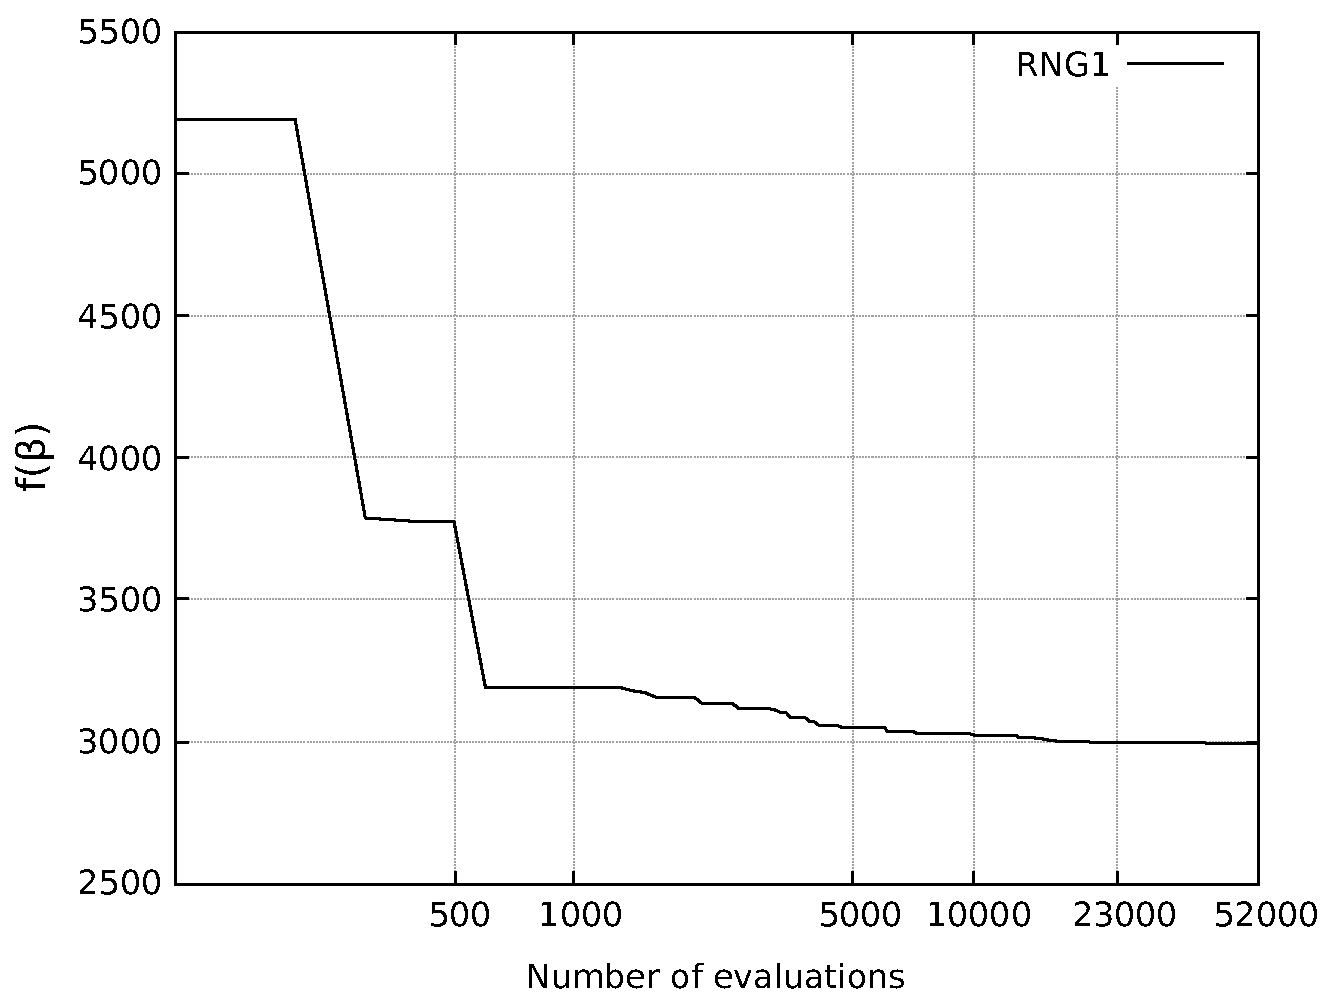
\includegraphics[width=\textwidth]{speed_reducer_ea_best.pdf}    
    \end{subfigure} 
\caption{Convergence history of speed reducer optimization case 
using EAs} 
\label{fig:EAs_speed_reducer}
\end{figure}

In 3 of the runs depicted in the previous figures, all 
evaluated individuals violate the imposed constraints in the first 
few generations and therefore their corresponding objective 
function values are penalised and do not appear in the range shown 
here. 

\newpage
%---------------------------------------------------------
%---------Off line------------
%----------------------------------------------------------

\begin{itemize}
\item \textbf{Optimization using MAEAs with metamodels trained 
off-line}
\end{itemize}

In MAEA-based optimization using off-line trained metamodels, both 
the objectives $\mathbf{F}(\vec{β})$ and the imposed constraints 
$\mathbf{C}(\vec{β})$ are approximated using surrogate models. 
Specifically, a global metamodel is built on the single objective 
and $n_{c}$ unique metamodels on each imposed constraint. 
Alternatively, a single surrogate model can be trained to 
approximate the entirety of the constraints with the same efficacy. 
In this case, the objective function is approximated by a KPLS 
model, while each constraint is approximated via the use of RBFs; 
responsible for the construction of the aforementioned metamodels 
is SMT software. In addition, the optimization of the speed reducer 
requires the formation of a mixed-integer design, since the number 
of teeth of the gear $n_{teeth}$ assumes strictly integer values. 
The outcome of the optimization through 5 runs is presented in 
table \ref{table:offline_speed_reducer}, where 20000 
evaluations per optimization cycle are performed utilizing the 
trained metamodel.
  
\begin{table}[h!]
\centering
%\rowcolors{2}{gray!30!}{white!50!gray!10}
\scalebox{0.83}{%
\begin{tabular}[c]{ |p{1.8cm}||p{1.6cm}|p{1.4cm}|p{1.4cm}|
p{1.8cm}|p{2.4cm}|p{1.4cm}|}
\toprule
\multicolumn{7}{|c|}{\cellcolor{gray!30!} 
\textbf{Speed reducer design}} \\
\midrule 
& $(μ,λ)$ \textbf{population} & \textbf{Best} 
& \textbf{Worst} & \textbf{Average} & \textbf{Average metamodel 
eval./cycle} & \textbf{Avg. cycles} \\
\hline
\textbf{MAEAs, off-line} & (30, 100) & 3000.95 & 3017.68
& 3006.01 & 20000 & 1 \\
\bottomrule
\end{tabular}%
}
\caption{Optimization of speed reducer design using MAEAs with 
off-line training}
\label{table:offline_speed_reducer}
\end{table}

The best candidate solution $\vec{β} = [3.502, 0.7, 17, 7.578, 
7.779, 3.357, 5.287]$ obtained via MAEAs with off-line training, 
produces the constraint and objective function values shown in 
table \ref{table:offline_error_speed_reducer} when evaluated on the 
PSM.

\begin{table}[h!]
\centering
%\rowcolors{2}{gray!30!}{white!50!gray!10}
\scalebox{0.82}{%
\begin{tabular}[c]{ |p{1.6cm}||p{2cm}|p{2cm}|p{2cm}|}
\toprule
\multicolumn{4}{|c|}{\cellcolor{gray!30!} 
\textbf{Speed reducer design}} \\
\midrule 
& \textbf{MAEAs, off-line} & \textbf{PSM} & \textbf{Relative Error}
\\
\hline
$\mathbf{c_{1}}(\vec{\bm{β}})$ & -0.077830 & -0.074335 & 0.045478
\\ 
$\mathbf{c_{2}}(\vec{\bm{β}})$ & -0.202314 & -0.198362 & 0.019438
\\
$\mathbf{c_{3}}(\vec{\bm{β}})$ & -0.442547 & -0.444165 & 0.003865
\\ 
$\mathbf{c_{4}}(\vec{\bm{β}})$ & -0.902293 & -0.902275 & 0.000004
\\
$\mathbf{c_{5}}(\vec{\bm{β}})$ & -0.004910 & -0.005490 & 0.120189
\\
$\mathbf{c_{6}}(\vec{\bm{β}})$ & -0.000146 & -0.000187 & 0.204286
\\ 
$\mathbf{c_{7}}(\vec{\bm{β}})$ & -0.702511 & -0.702500 & 0.000015
\\
$\mathbf{c_{8}}(\vec{\bm{β}})$ & -0.000203 & -0.000453 & 0.645450
\\
$\mathbf{c_{9}}(\vec{\bm{β}})$ & -0.584013 & -0.583144 & 0.001573
\\
$\mathbf{c_{10}}(\vec{\bm{β}})$ & -0.084767 & -0.084822 & 0.000209
\\
$\mathbf{c_{11}}(\vec{\bm{β}})$ & -0.008184 & -0.008183 & 0.005690
\\
$\mathbf{f}(\vec{\bm{β}})$ & 3000.95 & 3000.95 & 0\\
\bottomrule
\end{tabular}%
}
\caption{\textbf{C}, \textbf{F} responses to optimal $\vec{β}$ 
found via MAEAs with off-line training}
\label{table:offline_error_speed_reducer}
\end{table}

\newpage
%-------------------------------------------------------------


The deviation between metamodel predicted values and evaluated 
ones, using the exact PSM of either objective function or some 
constraint, can be observed in figures 
\ref{fig:fitting_f_speed_reducer},
\ref{fig:fitting_c1_4_speed_reducer}, 
\ref{fig:fitting_c5_11_speed_reducer}. The surrogate models are 
trained on $n_{t} \!= \!n_{doe} \!= \!150$ patterns $\mathbf{X}$ 
collected via the implementation of LHS scheme that makes use of 
the ESE algorithm to construct an optimal space-filling design. 
Each individual $\vec{β} \in P_{λ}^{0}$ selected via RNG1 is used 
to validate the trained model and calculate the NRMSE. 


\begin{figure}[h!]
\centering
    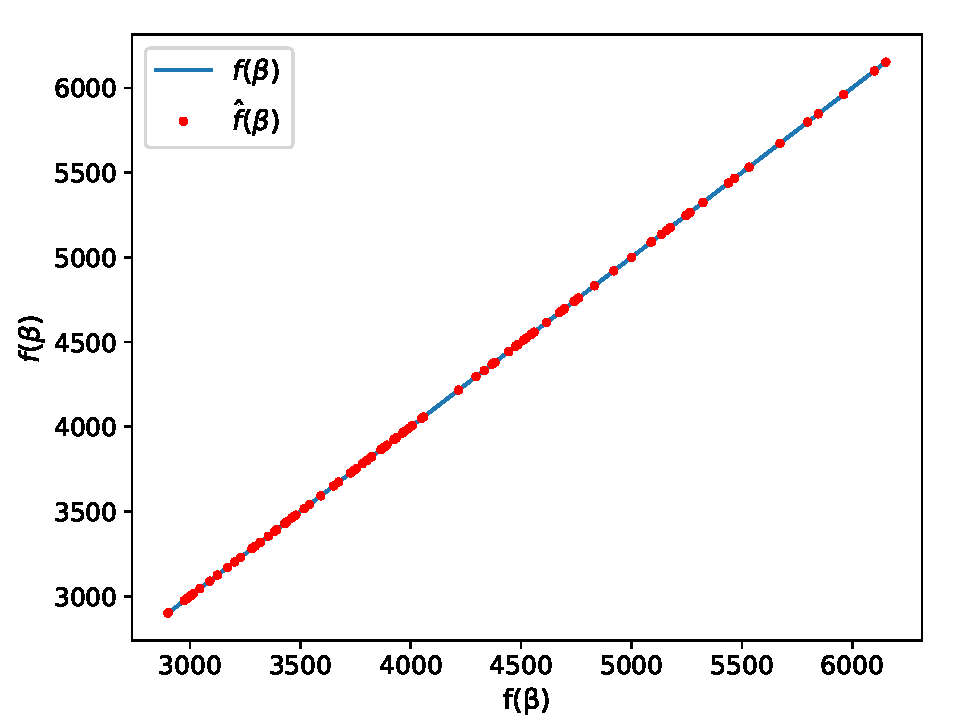
\includegraphics[width=0.44\textwidth]
    {speed_reducer_f_fitness.pdf}
    \caption{Speed reducer case with RNG1. Deviation between exact 
    PSM values of the objective function $\vec{f}(\vec{β})$ and 
    KPLS predictions $\hat{\vec{f}}(\vec{β})$ with NRMSE = 
    0.0000847}
\label{fig:fitting_f_speed_reducer}
\end{figure}


\begin{figure}[h!]
\centering
	\begin{subfigure}[b]{0.44\textwidth}
    \centering
    \caption{1st constraint, $\mathrm{NRMSE} \!= \!0.0082325$}
    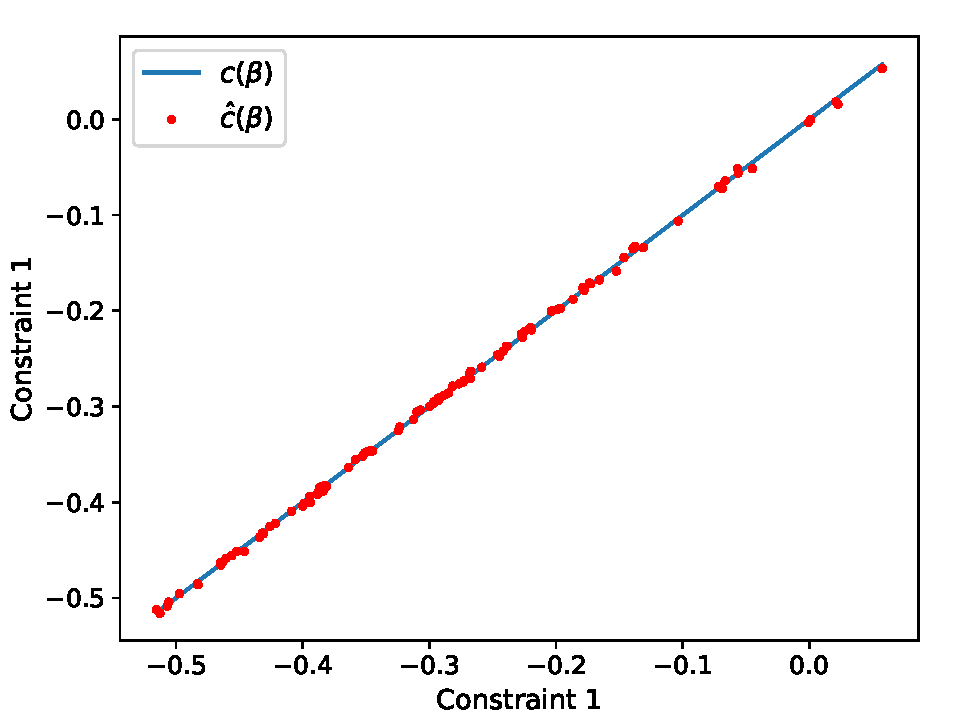
\includegraphics[width=\textwidth]
    {speed_reducer_con1_fitness.pdf}    
    \end{subfigure}
    \hfill
    \begin{subfigure}[b]{0.44\textwidth}
    \centering
    \caption{2nd constraint,$\mathrm{NRMSE} \!= \!0.0043814$}
    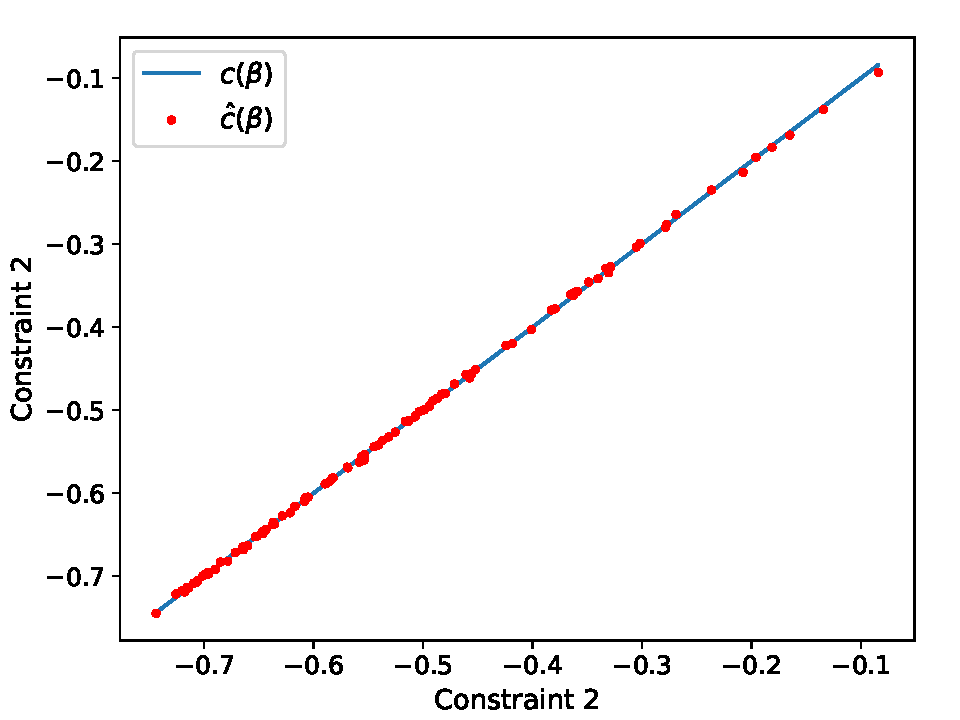
\includegraphics[width=\textwidth]
    {speed_reducer_con2_fitness.pdf}    
    \end{subfigure}
    \hfill
    \begin{subfigure}[b]{0.44\textwidth}
    \centering
    \caption{3rd constraint, $\mathrm{NRMSE} \!= \!0.0116700$}
    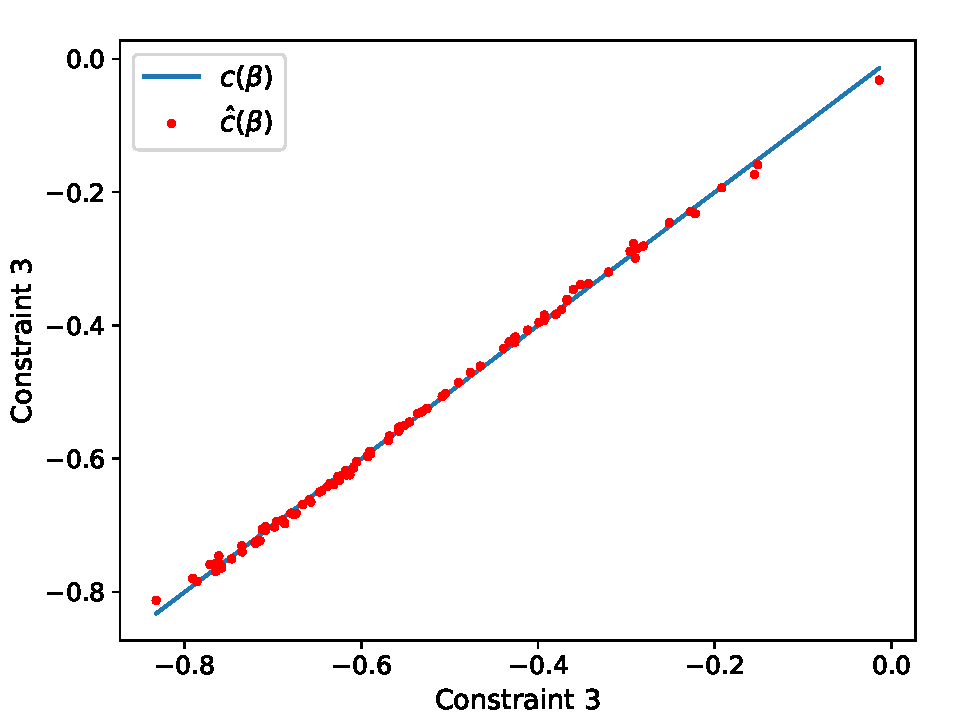
\includegraphics[width=\textwidth]
    {speed_reducer_con3_fitness.pdf}    
    \end{subfigure}
    \hfill
    \begin{subfigure}[b]{0.44\textwidth}
    \centering
    \caption{4th constraint, $\mathrm{NRMSE} \!= \!0.0002237$}
    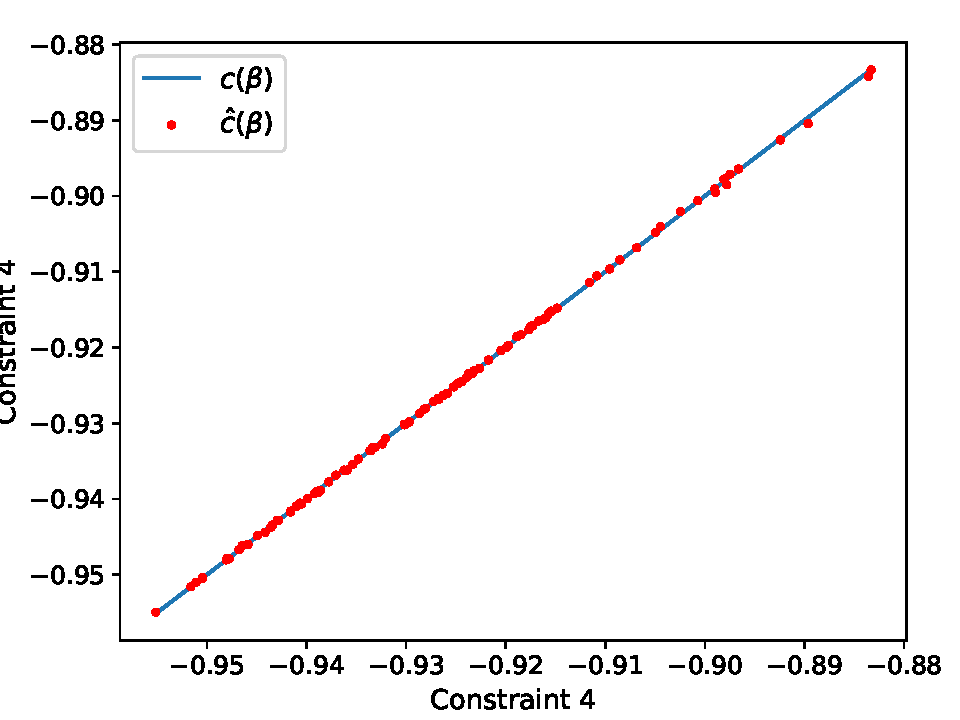
\includegraphics[width=\textwidth]
    {speed_reducer_con4_fitness.pdf}    
    \end{subfigure}
\caption{Deviation between exact PSM constraint values $\vec{c}
(\vec{β})$ and RBF predictions $\hat{\vec{c}}(\vec{β})$ given via 
the implementation of SMT. The results refer to the first four 
constraints in speed reducer case with RNG1.}
\label{fig:fitting_c1_4_speed_reducer}
\end{figure}

\newpage
%--------------------------------------------------------------


\begin{figure}[h!]
\centering
    \begin{subfigure}[b]{0.45\textwidth}
    \centering
    \caption{5th constraint, $\mathrm{NRMSE} \!= \!0.02209353$}
    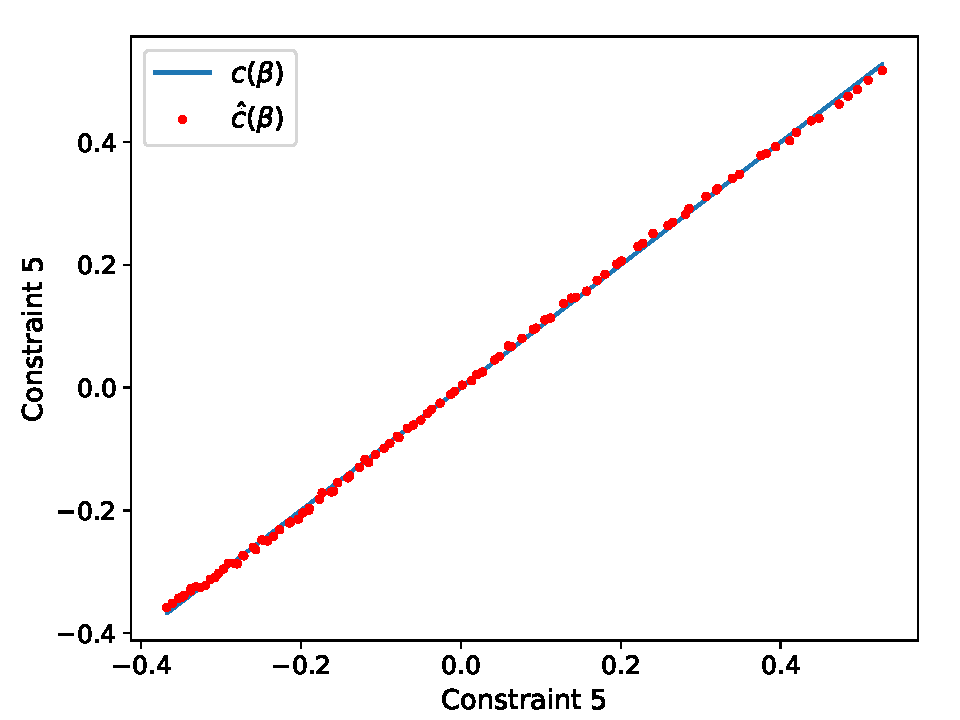
\includegraphics[width=\textwidth, height=0.6\textwidth, 
    scale=1]{speed_reducer_con5_fitness.pdf}    
    \end{subfigure}c
    \hfill
    \begin{subfigure}[b]{0.45\textwidth}
    \centering
    \caption{6th constraint, $\mathrm{NRMSE} \!= \!0.0031924$}
    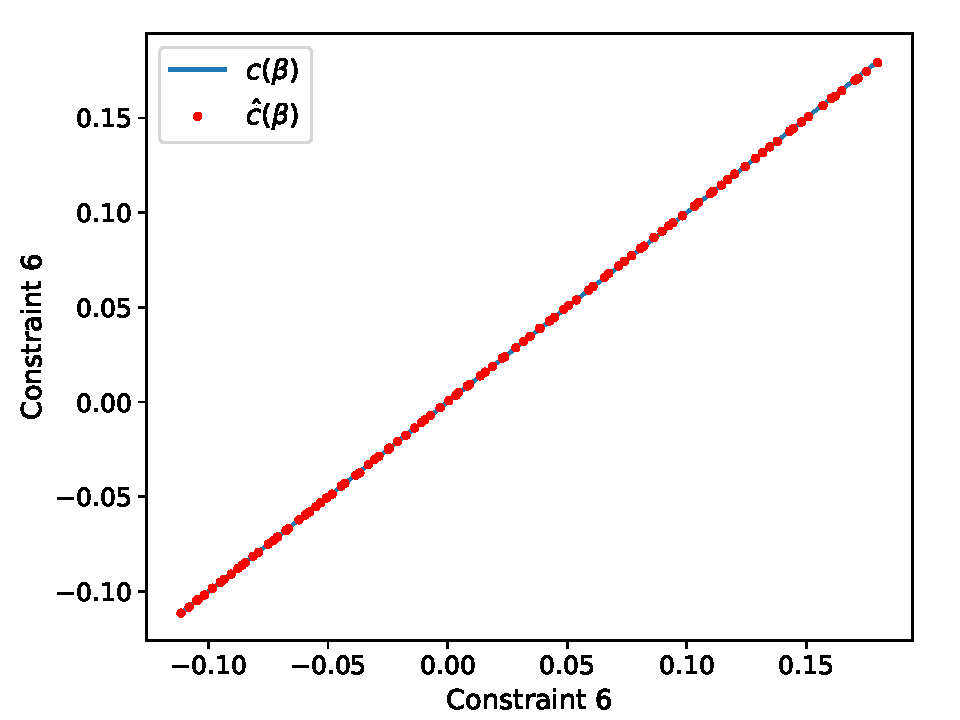
\includegraphics[width=\textwidth, height=0.6\textwidth, 
    scale=1]{speed_reducer_con6_fitness.pdf}    
    \end{subfigure}
    \hfill
    \begin{subfigure}[b]{0.45\textwidth}
    \centering
    \caption{7th constraint, $\mathrm{NRMSE} \!= \!0.0000092$}
    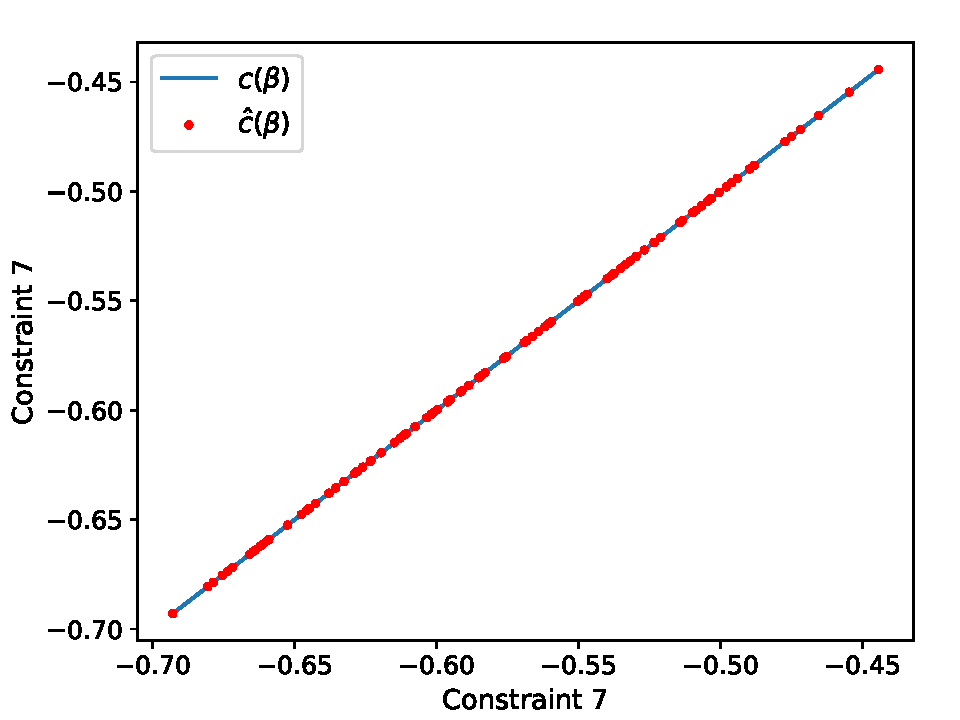
\includegraphics[width=\textwidth, height=0.6\textwidth, 
    scale=1]{speed_reducer_con7_fitness.pdf}    
    \end{subfigure}
    \hfill
    \begin{subfigure}[b]{0.45\textwidth}
    \centering
    \caption{8th constraint, $\mathrm{NRMSE} \!= \!0.0042978$}
    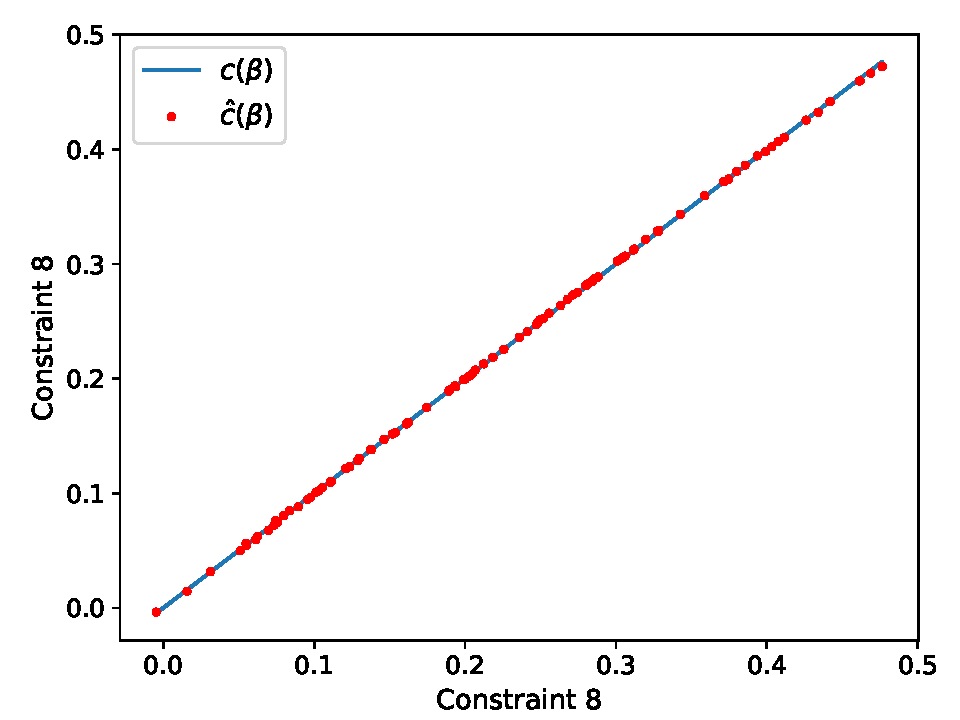
\includegraphics[width=\textwidth, height=0.6\textwidth, 
    scale=1]{speed_reducer_con8_fitness.pdf}    
    \end{subfigure}
    \hfill
    \begin{subfigure}[b]{0.45\textwidth}
    \centering
    \caption{9th constraint, $\mathrm{NRMSE} \!= \!0.0006251$}
    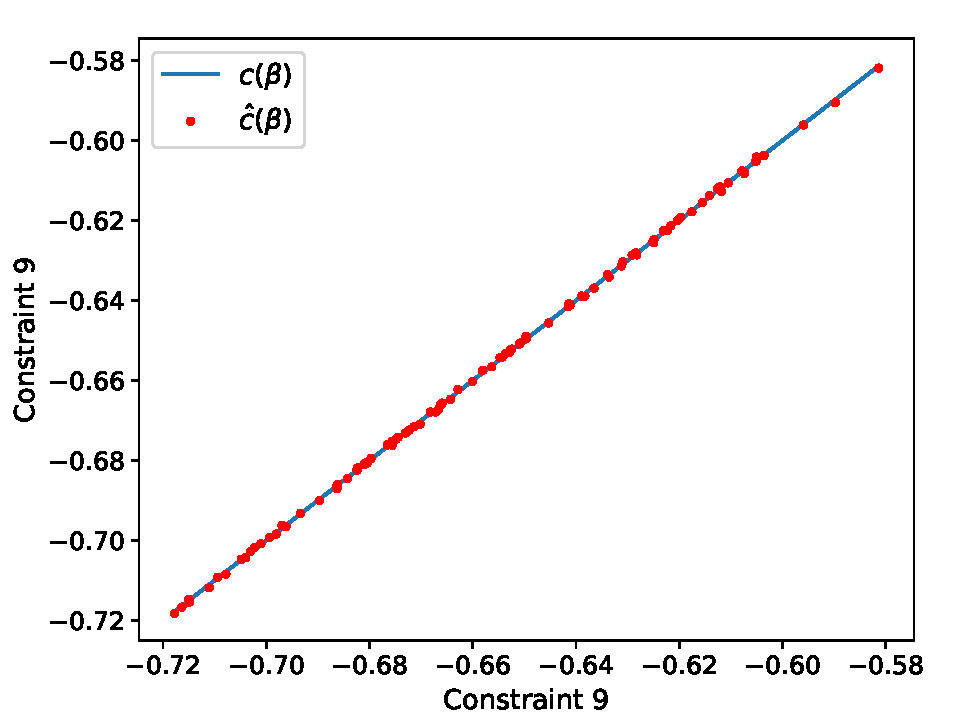
\includegraphics[width=\textwidth, height=0.6\textwidth, 
    scale=1]{speed_reducer_con9_fitness.pdf}    
    \end{subfigure}
    \hfill
    \begin{subfigure}[b]{0.45\textwidth}
    \centering
    \caption{10th constraint, $\mathrm{NRMSE} \!= \!0.0006814$}
    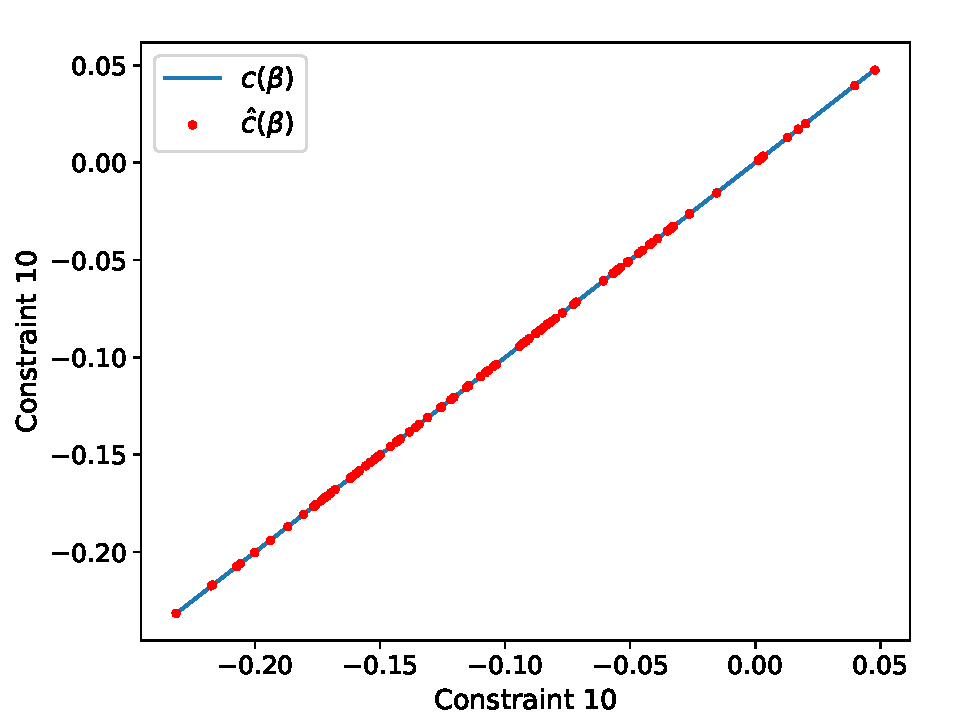
\includegraphics[width=\textwidth, height=0.6\textwidth, 
    scale=1]{speed_reducer_con10_fitness.pdf}    
    \end{subfigure}
    \hfill
    \begin{subfigure}[b]{0.45\textwidth}
    \centering
    \caption{11th constraint, $\mathrm{NRMSE} \!= \!0.0011311$}
    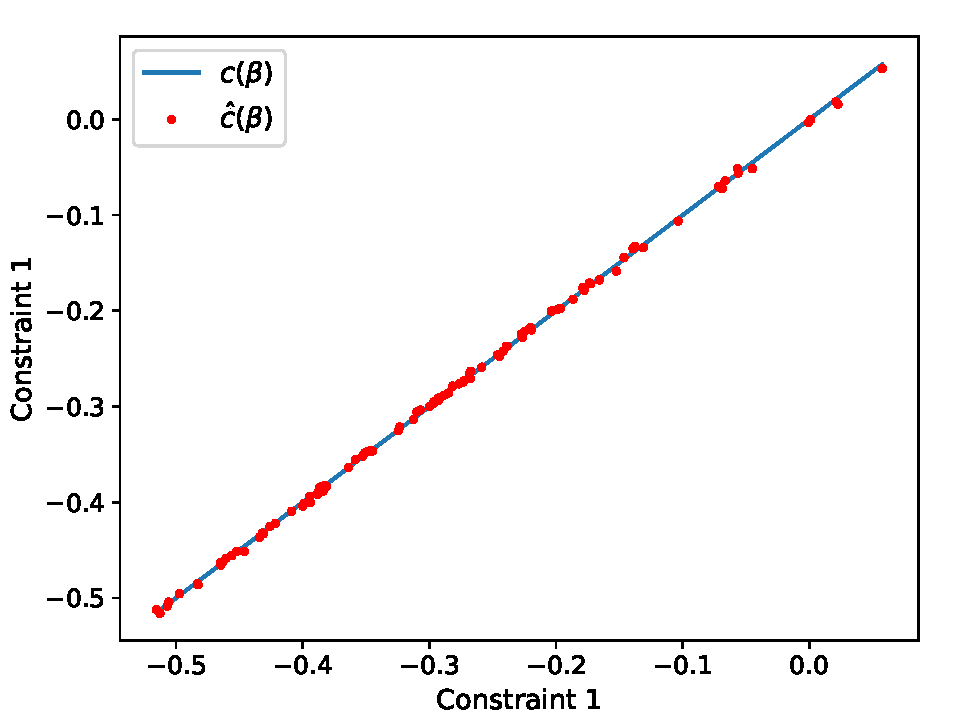
\includegraphics[width=\textwidth, height=0.6\textwidth, 
    scale=1]{speed_reducer_con1_fitness.pdf}    
    \end{subfigure}
\caption{Deviation between exact PSM constraint values $\vec{c}
(\vec{β})$ and RBF predictions $\hat{\vec{c}}(\vec{β})$ given via 
the implementation of SMT. The results refer to the remaining 
seven constraints in speed reducer case with RNG1.}
\label{fig:fitting_c5_11_speed_reducer}
\end{figure}

The NRMSE calculates the mean normalised deviation between the 
predicted and exactly evaluated on the PSM values on $λ=100$ 
untried design sites $\mathbf{Β}$, where $\vec{β} \!= \!
\vec{β}_{i} \!= \![β_{i,1}, β_{i,2}, \hdots, β_{i,n_{β}}] \in 
P_{λ}^{0}$ is any untried point in the design space contained in 
the initial offspring population set. NRMSE serves as a metric of 
model fitting and indicates that all trained metamodels are 
well-fitted, which explains why the optimization process converges 
after 1 cycle.

\newpage
%------------------------------------------------------------

%------------------------------------------------------------
%---------------On line----------------
%----------------------------------------------------------
\begin{itemize}
\item \textbf{Optimization using MAEAs with metamodels trained 
on-line}
\end{itemize}

In the MAEA-based optimization of welded beam design using on-line 
trained metamodels, the LCPE phase is set to initiate once 100 
exact PSM evaluations are performed. In LCPE, personalised local
metamodels are trained on $15 \leq n_{t} \leq 30$ training 
patterns and subsequently  $2 \leq λ_{e} \leq 4$ individuals
are re-evaluated using the exact evaluation model; a total of 
20000 PSM evaluations are performed. Local metamodels are built 
by utilising either the assisting software SMT or EASY. The former 
accommodates the use of Kriging, KPLS, KPLSK and RBFs, while the 
latter relies on Kriging and most often RBFs. In order to identify 
the most suitable metamodel in SMT for the speed reducer 
optimization case, a comparison between each respective model 
is performed w.r.t. the convergence history and the produced 
outcome; the results of each comparison are presented in table 
figure \ref{fig:SMT_models_speed_reducer} and table  
\ref{table:online_SMT_speed_reducer}, respectively.

\begin{figure}[h!]
\centering
	\begin{subfigure}[b]{0.49\textwidth}
	\centering
	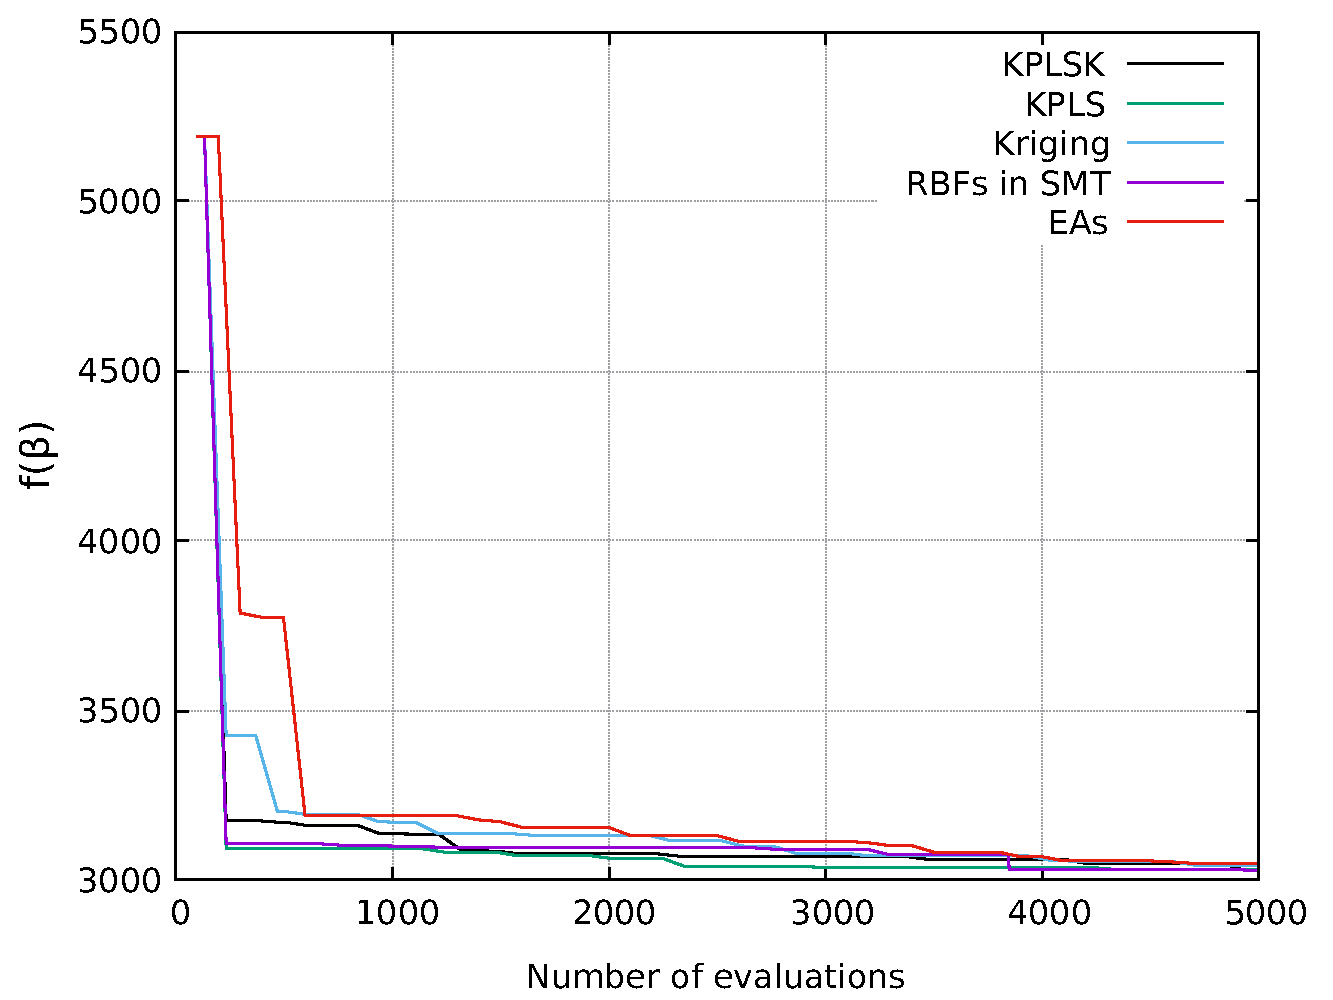
\includegraphics[width=\textwidth, height=0.85\textwidth, 
	scale=1]{speed_reducer_online_comparison.pdf}   
	\end{subfigure}
	\hfill
	\begin{subfigure}[b]{0.49\textwidth}
	\centering
	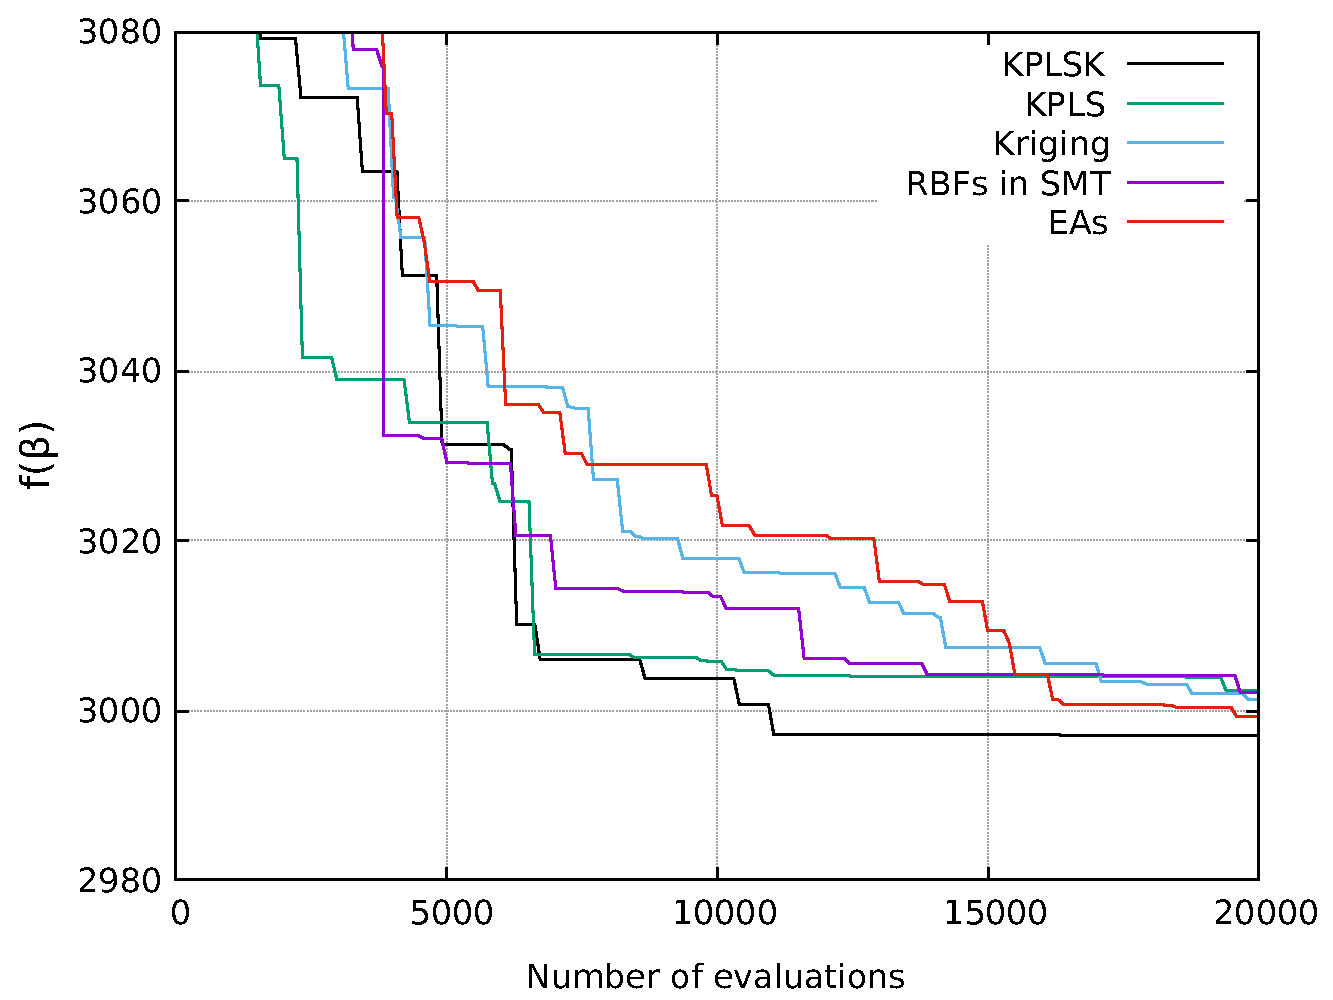
\includegraphics[width=\textwidth, height=0.85\textwidth, 
	scale=1]{speed_reducer_online_comparison2.pdf}   
	\end{subfigure}
\caption{Comparison between the convergence histories of speed 
reducer case using EAs and MAEAs with metamodels trained on-line 
via SMT} 
\label{fig:SMT_models_speed_reducer}
\end{figure}

\begin{table}[h!]
\centering
%\rowcolors{2}{gray!30!}{white!50!gray!10}
\scalebox{0.83}{%
\begin{tabular}[c]{ |p{1.6cm}||p{1.6cm}|p{1.8cm}|p{1.8cm}|
p{1.8cm}|p{2.2cm}|}
\toprule
\multicolumn{6}{|c|}{\cellcolor{gray!30!} 
\textbf{Speed reducer case}} \\
\midrule 
\textbf{MAEAs, on-line} & $(μ,λ)$ \textbf{population}  
& \textbf{KPLS} & \textbf{KPLSK} & \textbf{Kriging} 
& \textbf{RBFs} \\
\hline
\textbf{SMT} & (30, 100) & 3002.44 & 2997.06 & 3001.38 & 3002.14 \\
\bottomrule
\end{tabular}%
}
\caption{Speed reducer case with RNG1. Optimal candidate solution 
found using MAEAs with metamodels trained on-line via SMT}
\label{table:online_SMT_speed_reducer}
\end{table}

The comparison between convergence histories of the SMT built-in
metamodels, depicted in figure \ref{fig:SMT_models_speed_reducer},	 
indicates that KPLSK model is most suitable to 
facilitate the optimization of the speed reducer case due to its 
fast convergence to the threshold of both 10000 and 20000 PSM 
evaluations. In plain EAs, RNG1 yields the best optimization 
outcome and for that reason MAEAs with on-line training are 
initialized with the same offspring population $P_{λ}^{0}$.



\newpage
%----------------------------------------------------------------


KPLSK is yet to be compared to EASY built-in RBFs and plain EAs; 
the results are presented in table 
\ref{table:online_SMT_EASY_comparison_speed_reducer}.

\begin{table}[h!]
\centering
%\rowcolors{2}{gray!30!}{white!50!gray!10}
\scalebox{0.83}{%
\begin{tabular}[c]{ |p{2.2cm}||p{1.6cm}|p{2.2cm}|p{2.2cm}|
p{2.2cm}|p{1.6cm}|p{2.4cm}|}
\toprule
\multicolumn{7}{|c|}{\cellcolor{gray!30!} 
\textbf{Speed reducer case}} \\
\midrule 
\textbf{MAEAs, on-line} & $(μ,λ)$ \textbf{population}  
& \textbf{Best} & \textbf{Worst} & \textbf{Average} 
& \textbf{Average exact eval.} & \textbf{Avg. metamodel eval.} \\
\hline
\textbf{SMT} & (30, 100) & 2997.06 & 3005.35 & 3002.68 
& 20000 & 22792 \\
\textbf{EASY} & (30, 100) & 2998.53 & 3011.25 & 3005.46
& 20000 & 24775 \\
\hline
\textbf{Plain EAs} & (30, 100) & 2999.32 & 3008.35 & 3004.34 
& 20000 & - \\
\bottomrule
\end{tabular}%
}
\caption{Speed reducer case. Comparison between the outcome of the  
optimization using MAEAs with on-line training and plain EAs}
\label{table:online_SMT_EASY_comparison_speed_reducer}
\end{table}
  
The design variable vector that minimizes the weight of the speed 
reducer via the implementation of KLPSK is $\vec{β} = [3.501, 
0.7, 17, 7.348, 7.769, 3.352, 5.287]$. For MAEAs utilizing EASY 
built-in RBFs the respective optimal design variable vector is 
$\vec{β} = [3.503, 0.7, 17, 7.499, 7.750, 3.352, 5.287]$.

\begin{figure}[h!]
\centering
	\begin{subfigure}[b]{0.49\textwidth}
	\centering
	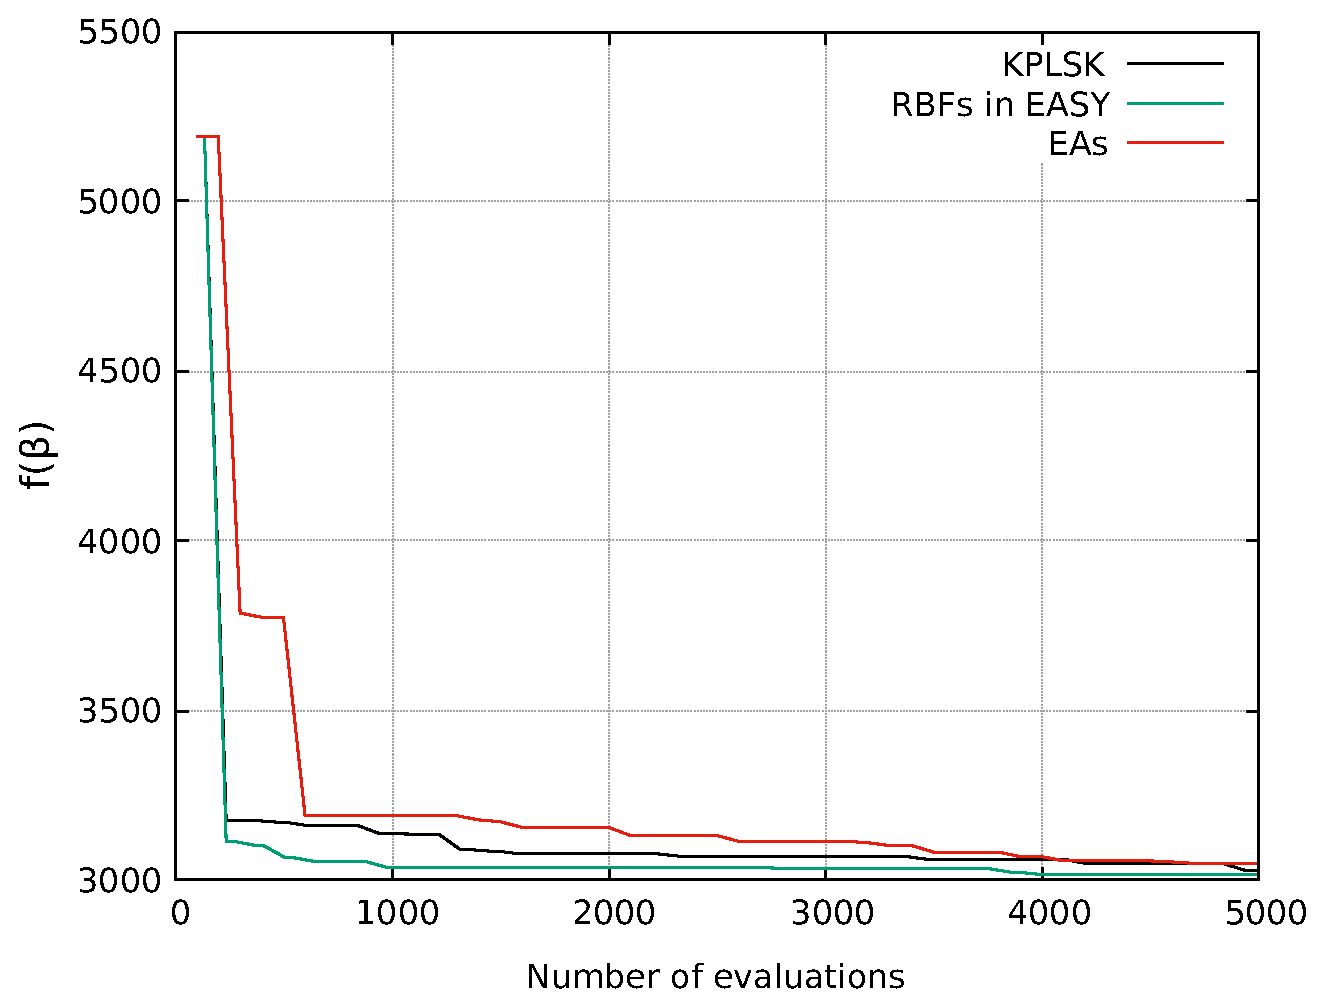
\includegraphics[width=\textwidth, height=0.85\textwidth, 
	scale=1]{speed_reducer_online.pdf}   
	\end{subfigure}
	\hfill
	\begin{subfigure}[b]{0.49\textwidth}
	\centering
	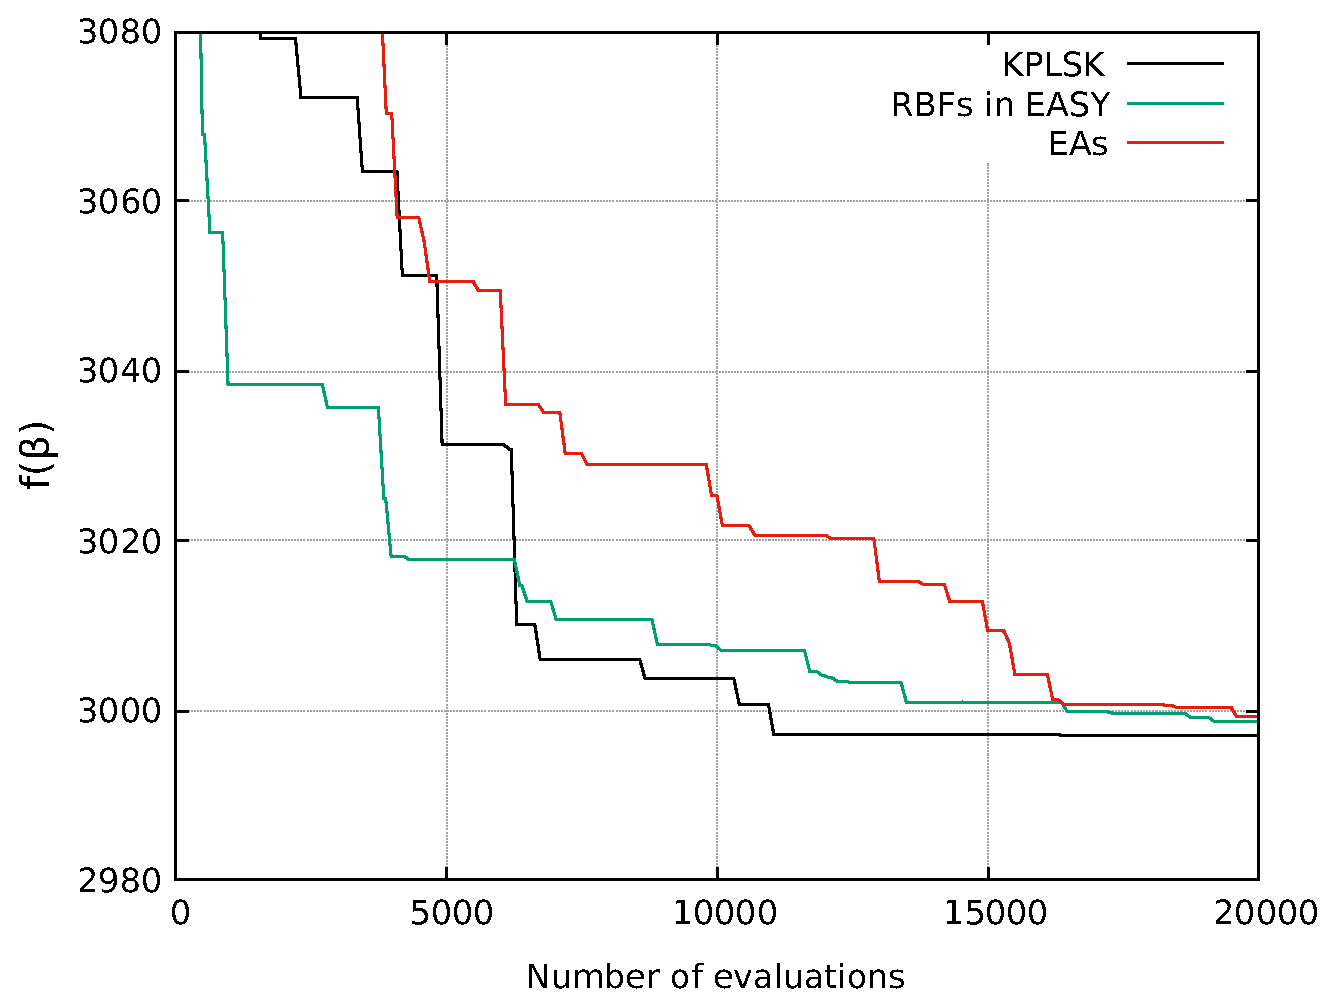
\includegraphics[width=\textwidth, height=0.85\textwidth, 
	scale=1]{speed_reducer_online2.pdf}   
	\end{subfigure}
\caption{Speed reducer case with RNG1. Comparison between the 
convergence of the optimization using MAEAs with on-line training 
and plain EAs} 
\label{fig:SMT_EASY_speed_reducer}
\end{figure}

In speed reducer optimization case, both MAEA methods 
outperform EAs and converge to a better optimal solution when 
compared prior to the threshold of 20000 PSM evaluations, as 
depicted in figure \ref{fig:SMT_EASY_speed_reducer}. Out of 
the two on-line trained MAEAs, KPLSK is seemingly the better option 
in the optimization of the speed reducer case, despite the fast 
convergence of EASY built-in RBFs for the first 6000 PSM 
evaluations. The optimization of the speed reducer case using MAEAs
with on-line trained KPLSK model resulted on average in a smaller
speed reducer weight, in comparison to conventional EAs and MAEAs
with EASY built-in, on-line trained RBFs.


\newpage
%--------------------------------------------------------


\section{Analysis of the SOO outcome}
The results and observations made during the study will 
subsequently be included in the analysis of the performance of each 
MAEA method and each utilized metamodel. The performance of each 
model or method is measured by two conflicting objectives, i.e. 
model/method efficacy and computational cost. The former can be 
quantified by observing the convergence of each model, while 
the latter can be measured via the wall clock time needed to 
preform each process related to the optimization. The results 
regarding these two objectives are presented subsequently.\\

\begin{itemize}

\item \textbf{Convergence} \\
The plot of convergence histories can be used in the 
comparison of methods that evaluate the evolution individuals on 
the exact PSM, therefore, MAEAs with off-line training cannot 
effectively be compared using this method. For this reason, the 
yielded outcome of each method is compared. In welded beam case,
MAEAs with on-line training perform significantly better 
than the ones with off-line training due to poor fitting of the 
metamodels approximating the constraint functions. MAEAs with 
EASY built-in RBFs trained on-line outperform plain EAs and 
MAEAs using metamodels trained on-line via SMT when 
compared prior to the threshold of 10000 PSM evaluations.

In the speed reducer case MAEA-based optimization, off-line trained 
metamodels well-fitted and yield a similar average outcome compared 
to plain EAs after 5 runs. MAEAs with on-line training, however, 
outperform both methods, i.e. EAs and MAEAs with off-line training. 


\item \textbf{Total function calls} \\
The total wall clock time depends heavily on the number of 
exact PSM evaluations performed, so it is necessary to calculate 
the total amount of PSM evaluations performed by each optimization 
method. In MAEAs with off-line training, the number of initial 
sample points selected via DoE techniques is equal to $n_{doe} \!= 
\!240$ and $n_{doe} \!= \!150$ for the welded beam and the speed 
reducer design, respectively, while the average number of PSM 
evaluations is calculated as such:
\begin{equation}
\overline{n}_{PSM} = n_{doe} + (n_{cycles} - 1)n_{doe}^{'} + 
n_{elites}
\end{equation}

In the previous formula, $n_{elites}$ is the total number of elite 
individuals selected throughout the optimization process, which 
for SOO problems is equal to the number of cycles performed, 
since a single elite individual is selected in each cycle. In 
welded beam optimization case, an average of $\overline{n}
_{PSM^{''}} = 240 + 7 \!\cdot \!20 + 8 = 388$ $\mathrm{PSM}^{''}$ 
evaluations were performed, while in speed reducer case the 
respective PSM evaluations are $\overline{n}_{PSM} = 151$. 
In comparison, EAs and MAEAs with on-line training used for the 
minimization of welded beam case perform an average of 
$\overline{n}_{PSM} \!= \!10000$ evaluations respectively. In speed 
reducer case, the corresponding exact PSM evaluations performed are 
$\overline{n}_{PSM} \!= \!20000$. This decrease in exact 
evaluations, when compared to conventional EAs and MAEAs with 
on-line training, yields a proportional reduction in computational 
cost, making MAEAs with off-line training the most cost-efficient 
optimization method.

\end{itemize}

\newpage
%-----------------------------------------------------------------


In MAEAs with on-line or off-line training, metamodel approximation 
is used, which contributes in an insignificant increase in the 
total wall clock time compared to the exact evaluation performed by 
the PSM. Consequently, the total function calls must account for 
the number of times the Python or C++ function that is responsible 
for the metamodel prediction was called; the corresponding number 
is denoted by $\overline{n}_{meta}$. The total number of function 
calls, i.e. $\overline{n}_{PSM}$ and $\overline{n}_{meta}$, along 
with the average outcome of each optimization method, is presented 
in table \ref{table:pseudo_engineering_outcome}.

\begin{table}[h!]
\centering
%\rowcolors{2}{gray!30!}{white!50!gray!10}
\scalebox{0.83}{%
\begin{tabular}[c]{ |p{3.8cm}||p{2.8cm}|p{1cm}|p{1cm}||p{3cm}|
p{1cm}|p{1cm}|}
\toprule
\multicolumn{7}{|c|}{\cellcolor{gray!30!} 
\textbf{Average outcome}} \\
\midrule 
& \textbf{Welded beam} & $\mathbf{\overline{n}_{PSM}}$ 
& $\mathbf{\overline{n}_{meta}}$
& \textbf{Speed reducer} & $\mathbf{\overline{n}_{PSM}}$ 
& $\mathbf{\overline{n}_{meta}}$ \\
\hline
\textbf{MAEAs, on-line training via SMT} & 2.54 & 10000 & 11579
& 3002.68 & 20000 & 22792 \\
\textbf{MAEAs, on-line training via EASY} & 2.53 & 10000 & 14422
& 3005.46 & 20000 & 24775 \\
\textbf{EAs} & 2.59 & 10000 & - & 3004.34 & 20000 & - \\
\textbf{MAEAs, off-line training via SMT} & 3.12 & 388 & 23064 
& 3006.01 & 151 & 18239 \\
\bottomrule
\end{tabular}%
}
\caption{Comparison between the average optimization outcome using 
plain EAs, MAEAs with on-line and off-line training after 5 runs}
\label{table:pseudo_engineering_outcome}
\end{table}

%\item \textbf{Wall clock time} \\
%The computational cost refers to the wall 
%clock time of each individual process performed in order to train
%and use the metamodel. The most important processes are the 
%construction of the DoE, i.e. sampling phase, the evaluation on %the 
%exact PSM, the training of the surrogate model, the evaluation of 
%the selected elites on the exact PSM and the prediction using the 
%trained metamodel. The wall clock time of each process corresponds 
%to the time needed for each process to be executed. The results 
%were measured using the multi-processor platform of the 
%PCOpt/NTUA and are subsequently presented in the following table:

%\begin{table}[h!]
%\centering
%%\rowcolors{2}{gray!30!}{white!50!gray!10}
%\scalebox{0.81}{%
%\begin{tabular}[c]{ |p{2.4cm}||p{1.8cm}|p{1.2cm}|p{1.2cm}|
%p{1.8cm}||p{1.8cm}|p{1.2cm}|p{1.2cm}|p{1.8cm}|}
%\toprule
%\multicolumn{5}{|c||}{\cellcolor{gray!30!} 
%\textbf{Welded beam case}} &
%\multicolumn{4}{|c|}{\cellcolor{gray!30!} 
%\textbf{Speed reducer case}} \\
%\midrule 
%& \textbf{Wall clock time/process [s]} 
%& $\mathbf{\overline{n}_{PSM}}$ & $\mathbf{\overline{n}_{meta}}$
%& \textbf{Total wall clock time [s]}
%& \textbf{Wall clock time/process [s]} 
%& $\mathbf{\overline{n}_{PSM}}$ & $\mathbf{\overline{n}_{meta}}$
%& \textbf{Total wall clock time [s]} \\
%\hline
%\multicolumn{9}{|c|}{\cellcolor{gray!15!} \textbf{EAs}} \\
%\textbf{PSM eval.} & 0.333 & 10000 & - & 3330
%& 0.358 & 20000 & - & 7160 \\
%\hline
%\multicolumn{9}{|c|}{\cellcolor{gray!15!} \textbf{MAEAs with 
%metamodels trained off-line via SMT}} \\
%\textbf{Sampling} & 0.859 & - & 8 & 6.872
%& 1.231 & - & 1 & 1.231 \\
%\textbf{PSM eval.} & 0.318 & 388 & - & 123.384
%& 0.347 & 151 & - & 52.397 \\
%\textbf{F Training} & 1.423 & - & 8 & 11.384
%& 1.446 & - & 1 & 1.446 \\
%\textbf{C training} & 1.563 & - & 8 & 12.504
%& 1.586 & - & 1 & 1.586 \\
%\textbf{Prediction} & 1.547 & - & 23064 & 26223.768
%& 1.553  & - & 18239 & 28325.167 \\
%\hline
%\multicolumn{9}{|c|}{\cellcolor{gray!15!} \textbf{MAEAs with 
%metamodels trained on-line via SMT}} \\
%\textbf{PSM eval.} & 0.249 & 10000 & - & 2490
%& 0.289 & 20000 & - & 5780 \\
%\textbf{Training} & 1.443 & - & 11579 & 16708.497
%& 1.551 & - & 22792 & 35350.392 \\
%\textbf{Prediction} & 1.137 & - & 11579 & 13165.323
%& 1.217 & - & 22792 & 27737.864 \\
%\hline
%\multicolumn{9}{|c|}{\cellcolor{gray!15!} \textbf{MAEAs with 
%metamodels trained on-line via EASY}} \\
%\textbf{PSM eval.} & 0.112 & 10000 & - & 1120
%& 0.128 & 20000 & - & 2560 \\
%\textbf{Training} & 0.257 & - & 14422 & 3706.454
%& 0.304 & - & 24775 & 7532.6 \\
%\textbf{Prediction} & 0.102 & - & 14422 & 1471.044
%& 0.115 & - & 24775 & 2849.125 \\
%\bottomrule
%\end{tabular}%
%}
%\caption{Wall clock time of each individual process as measured 
%when using the KPLS model}
%\label{table:wall_clock_time}
%\end{table}

%\newpage
%%---------------------------------------------------------------


%The prediction phase in MAEAs with off-line training includes the 
%prediction of both the objective function and the constraints. For 
%this reason its duration must be shorter than the total time 
%required to train $\mathbf{F}$ and $\mathbf{C}$. On-line trained 
%surrogate models, on the other hand, are built exclusively on the 
%objective function and thus wall clock time of each prediction is 
%shorter. 

%On table \ref{table:wall_clock_time} are featured three different 
%exact PSM evaluation wall clock times. In an optimization %utilizing 
%plain EAs, the time needed to perform an exact PSM evaluation is 
%the longest, since the corresponding script is written in Python 
%and contains the code for computing the objective function and the 
%imposed constraints, along with other Python modules.

%In MAEAs with off-line training, the average number of metamodel 
%cycles per evaluation is equal to 2883 and 18239 in the welded %beam 
%and in the speed reducer case, respectively. Consequently, if 
%multiplied the number of average cycles $n_{cycles}$ the average 
%number of predictions performed will be equal to 23064 and 18239, 
%respectively. In MAEAs using metamodels tained on-line via SMT, 
%Python is the main coding language used and thus the computational 
%cost of executing the corresponding \textit{evaluation.py} %reamains
%high, but slightly lower than that amounting after using plain %EAs.
%The optimization that utilizes RBFs trained on-line via EASY is 
%performed using entirely C++ and, thus, its cost is the lowest.

%The wall clock time of the processes performed by 
%each metamodel utilized via SMT is presented in the following 
%table:

%\begin{table}[h!]
%\centering
%%\rowcolors{2}{gray!30!}{white!50!gray!10}
%\scalebox{0.83}{%
%\begin{tabular}[c]{ |p{2.5cm}||p{2.2cm}|p{2.2cm}|p{2.2cm}|
%p{2.2cm}|}
%\toprule
%\multicolumn{5}{|c|}{\cellcolor{gray!30!} 
%\textbf{Wall clock time [s]}} \\
%\midrule 
%& \textbf{Kriging} & \textbf{KPLS} & \textbf{KPLSK} & \textbf{RBF} 
%\\
%\hline
%\textbf{Training} & 1.679 & 1.443 & 1.939 & 1.294 \\
%\textbf{Prediction} & 1.137 & 1.137 & 1.137 & 1.131 \\
%\bottomrule
%\end{tabular}%
%}
%\caption{Wall clock time needed to construct and use each 
%metamodel}
%\end{table}

%Consequently, the results in table \ref{table:wall_clock_time} can 
%be restated accordingly in order to correspond to KPLSK, Kriging %or 
%RBF. The entirety of the aforementioned results is combined in 
%the following table:
%\end{itemize}

%\begin{table}[h!]
%\centering
%%\rowcolors{2}{gray!30!}{white!50!gray!10}
%\scalebox{0.83}{%
%\begin{tabular}[c]{ |p{3.8cm}||p{2.2cm}|p{2cm}|p{1.3cm}||
%p{2.2cm}|p{2cm}|p{1.3cm}|}
%\toprule
%\multicolumn{4}{|c|}{\cellcolor{gray!30!} 
%\textbf{Welded beam design}} &
%\multicolumn{3}{|c|}{\cellcolor{gray!30!} 
%\textbf{Speed reducer design}} \\
%\midrule 
%& \textbf{Wall clock time} & \textbf{Average} 
%$\vec{\mathbf{f}}$ & $\mathbf{\overline{n}_{PSM}}$ 
%& \textbf{Wall clock time} & \textbf{Average} 
%$\vec{\mathbf{f}}$ & $\mathbf{\overline{n}_{PSM}}$ \\
%\hline
%\textbf{MAEAs, on-line training via SMT} & 8 h 59 min & 2.54 
%& 10000 & 19 h 17 min & 3002.68 & 20000 \\
%\textbf{MAEAs, on-line training via EASY} & 1 h 45 min & 2.86 
%& 10000 & 3 h 36 min & 3005.46 & 20000 \\
%\textbf{EAs} & 56 min & 2.59  & 10000 
%& 1 h 59 min & 3004.34 & 20000 \\
%\textbf{MAEAs, off-line training via SMT} & 7 h 20 min & 3.12 
%& 388 & 7 h 53 min & 3006.01 & 151 \\
%\bottomrule
%\end{tabular}%
%}
%\caption{Comparison between all implemented optimization methods}
%\end{table}

MAEAs using metamodels trained on-line via SMT yield the best 
optimization outcome, increase significantly, however, the 
computational cost of the process. The high computational cost, 
also observed in MAEAs trained off-line via SMT, is contributed to 
the implementation of Python in the optimization process. Python
is built dynamically, i.e. the data types are determined at run 
time, on an interpreter, unlike other coding languages that are 
pre-compiled, e.g. C++ that EASY is based on. Both these 
attributes, along with the use of several custom functions, prolong 
the wall clock time needed for each process to be executed.
Another factor in the increase of the computational cost is the 
evaluation of each offspring individually; if the entirety of the 
population in a generation was being evaluated, then the cost would 
decrease $λ$-fold. Consequently, the implementation of SMT and any 
other Python-based package that utilizes metamodels is not 
recommended for pseudo-engineering applications with low-order 
objective functions. MAEAs with on-line trained RBFs found in EASY 
are based on C++ and their use does not increase the computational 
cost of the optimization significantly. They additionally converge 
faster than conventional EAs and MAEAs using SMT metamodels 
trained either on-line or off-line, and their use is preferred in 
simple pseudo-engineering cases.